%%%%%%%%%%%%%%%%%%%%%%%%%%%%%%%%%%%%%%%%%%%%%%%%%%%%%%%%%%%%%%%%%%%%%%%%%%%
\chapter{Methodology}
%%%%%%%%%%%%%%%%%%%%%%%%%%%%%%%%%%%%%%%%%%%%%%%%%%%%%%%%%%%%%%%%%%%%%%%%%%%

\section{Development Model}
In the development process of the system, the developers will utilize the Rapid Application Development (RAD) model as a project management strategy. This methodology is characterized by an iterative approach in the software development process, which begins with the specification of requirements from the users and proceeds through rapid prototyping iterative delivery, and continual maintenance for the currently completed software. This methodology is well-suited for the study as it provides researchers a clear overview to follow from the beginning to the end, making it easier to track each step's progress as well as make sure everything went according to the plan. Moreover, the RAD model is perfect to use for projects with expedited schedules and evolving requirements as it lays a strong emphasis on speed, adaptability, and user-centric design. 

The implementation of RAD provides a substantial advantage in developing the HRIS application. In terms of speed in development, RAD makes it possible to develop and release new features, which makes it ideal for projects with tight deadlines. And because of its adaptability, it can accommodate changes in requirements even at the end of the development cycle, guaranteeing that the result fulfills the requirements of the users. With the user-centric nature of RAD, it includes user feedback in every iteration, which could increase user satisfaction with the finished product. Furthermore, this methodology includes a risk reduction aspect which implies that early prototypes can help in recognizing any potential issues and reducing risks associated with functionality and usability. Due to RAD's iteration methodology, the HRIS system may be continuously improved in response to user feedback and changing educational requirements, keeping it updated and efficient in providing the desired outcomes.

\begin{figure}[H]
    \centering
    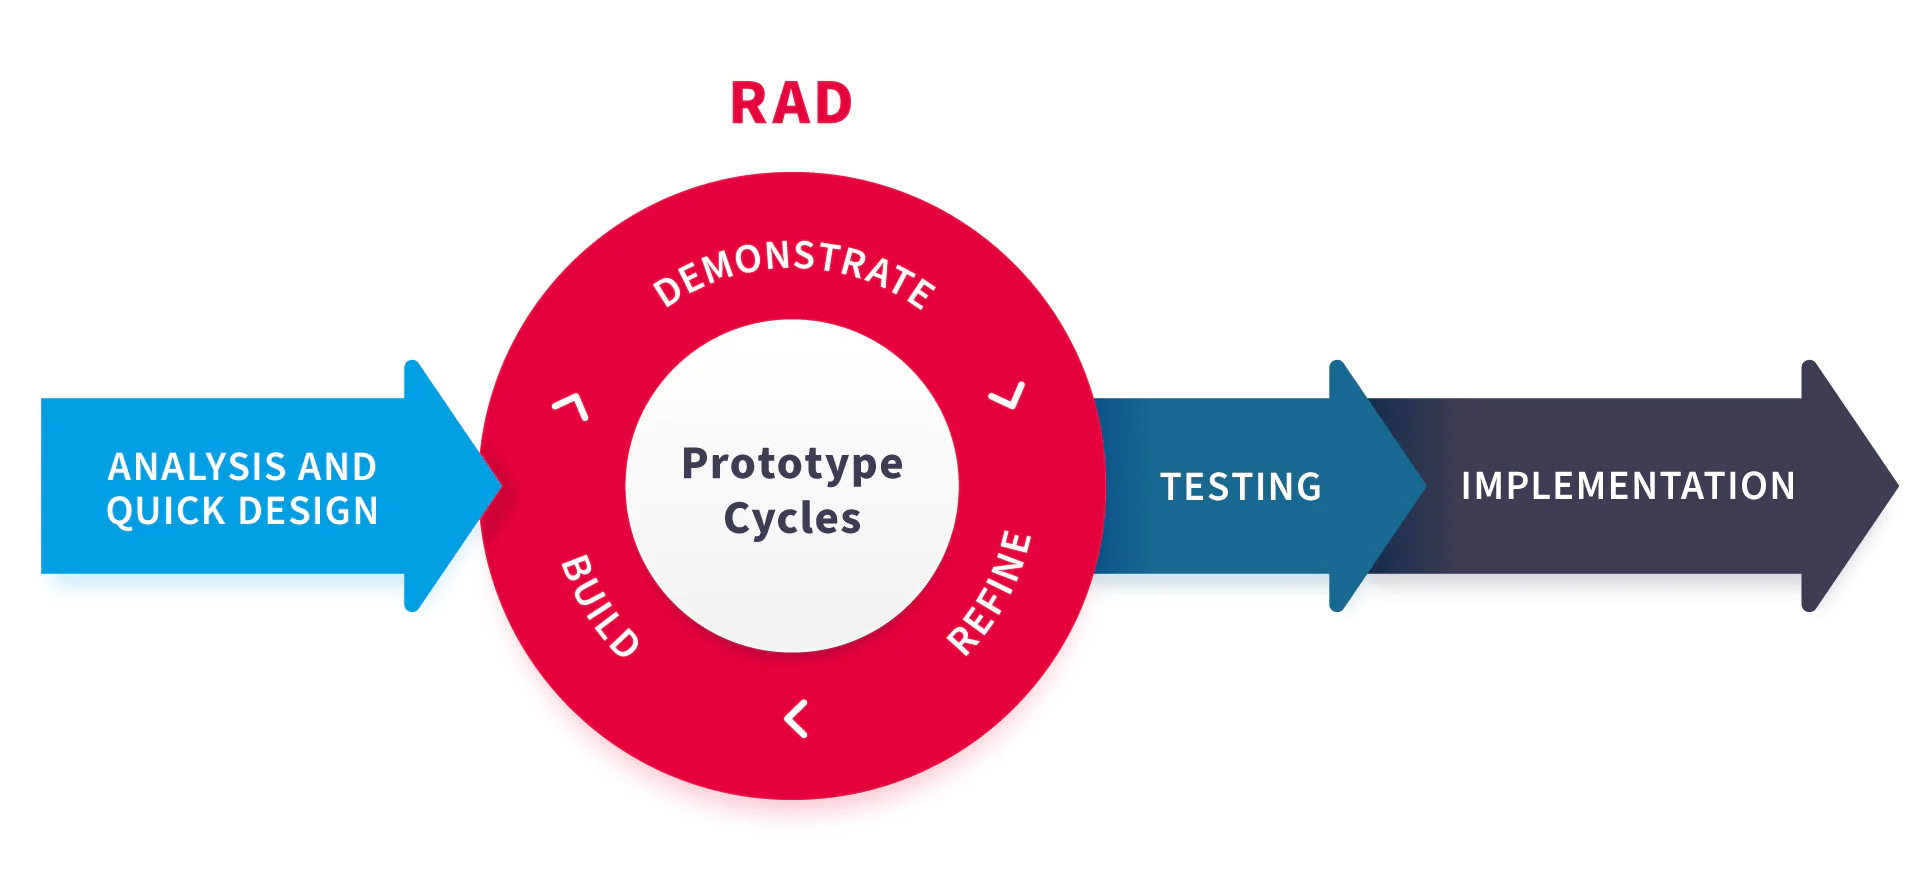
\includegraphics[width=1\linewidth]{figures/images/doc/rad.png}
    \caption{Rapid Application Development (RAD) Model.}
    \label{fig:rad}
\end{figure}
    
\section{System Analysis}
The system analysis phase of the HRIS application development involves utilizing various methods to understand and define the system's functional and data requirements. These include information gathering, analytical methods, personnel consultation assessments, and content analysis. These methods aid in identifying user needs, defining system functionalities, and establishing the database schema. 

Through the use of visual tools i.e., Swim-lane Diagram, Use case Diagrams, Entity Relational Diagrams, and Gantt charts, the system analysis phase enables a comprehensive understanding of the HRIS application's scope and requirements. By employing a systematic approach to system analysis, the development team can ensure that the HRIS application is designed and implemented in alignment with the project objectives and user expectations.

\subsection{Organizational Structure}

The ADNU HRMO currently maintains an organizational structure, with each role clearly defined to ensure efficient management and operation of the HRIS. Each role has specific responsibilities and access levels within the HRIS, ensuring that the system operates smoothly and effectively.

\begin{figure}[H]
    \centering
    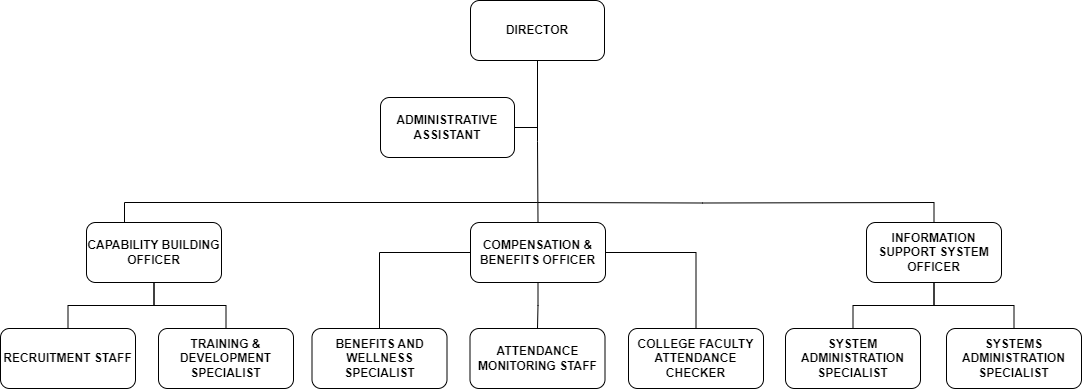
\includegraphics[width=1\linewidth]{figures/images/doc/organizational-structure.png}
    \caption{HRIS Organizational Structure.}
    \label{fig:organizational-struct}
\end{figure}

With this organizational structure in place, the new system will be designed to accommodate the roles and responsibilities of each HR staff member present in the structure figure \ref*{fig:organizational-struct}. 

    \subsection{Swim-lane Diagram}
    The Swim-lane diagram illustrates the process flow of the HRIS. The process begins when the user enters their login credentials. These credentials are unique to each University personnel, distinguishing them from other users in the system. Each user has different privileges and assignments set initially to access the system. After entering the credentials, the system validates them, granting the user access to the system. Once the user successfully logs in, they are directed to the dashboard where they can perform different actions depending on their privileges e.g., perform employee actions or tasks and HR overall general management.

    The identified roles i.e., Director, Sys. Admin, Attendance Monitoring and Checker, Training \& Dev. Specialist, Records Mgt. Specialist, Comp. \& Benefits Officer, ISS Officer, Recruitment \& Admin Staff, and Capability Bldg. Officer, are assigned specific tasks and responsibilities within the system. These responsibilities and privileges are outlined in table \ref*{tab:hris-basic-modules}. 

    \begin{figure}[H]
        \centering
        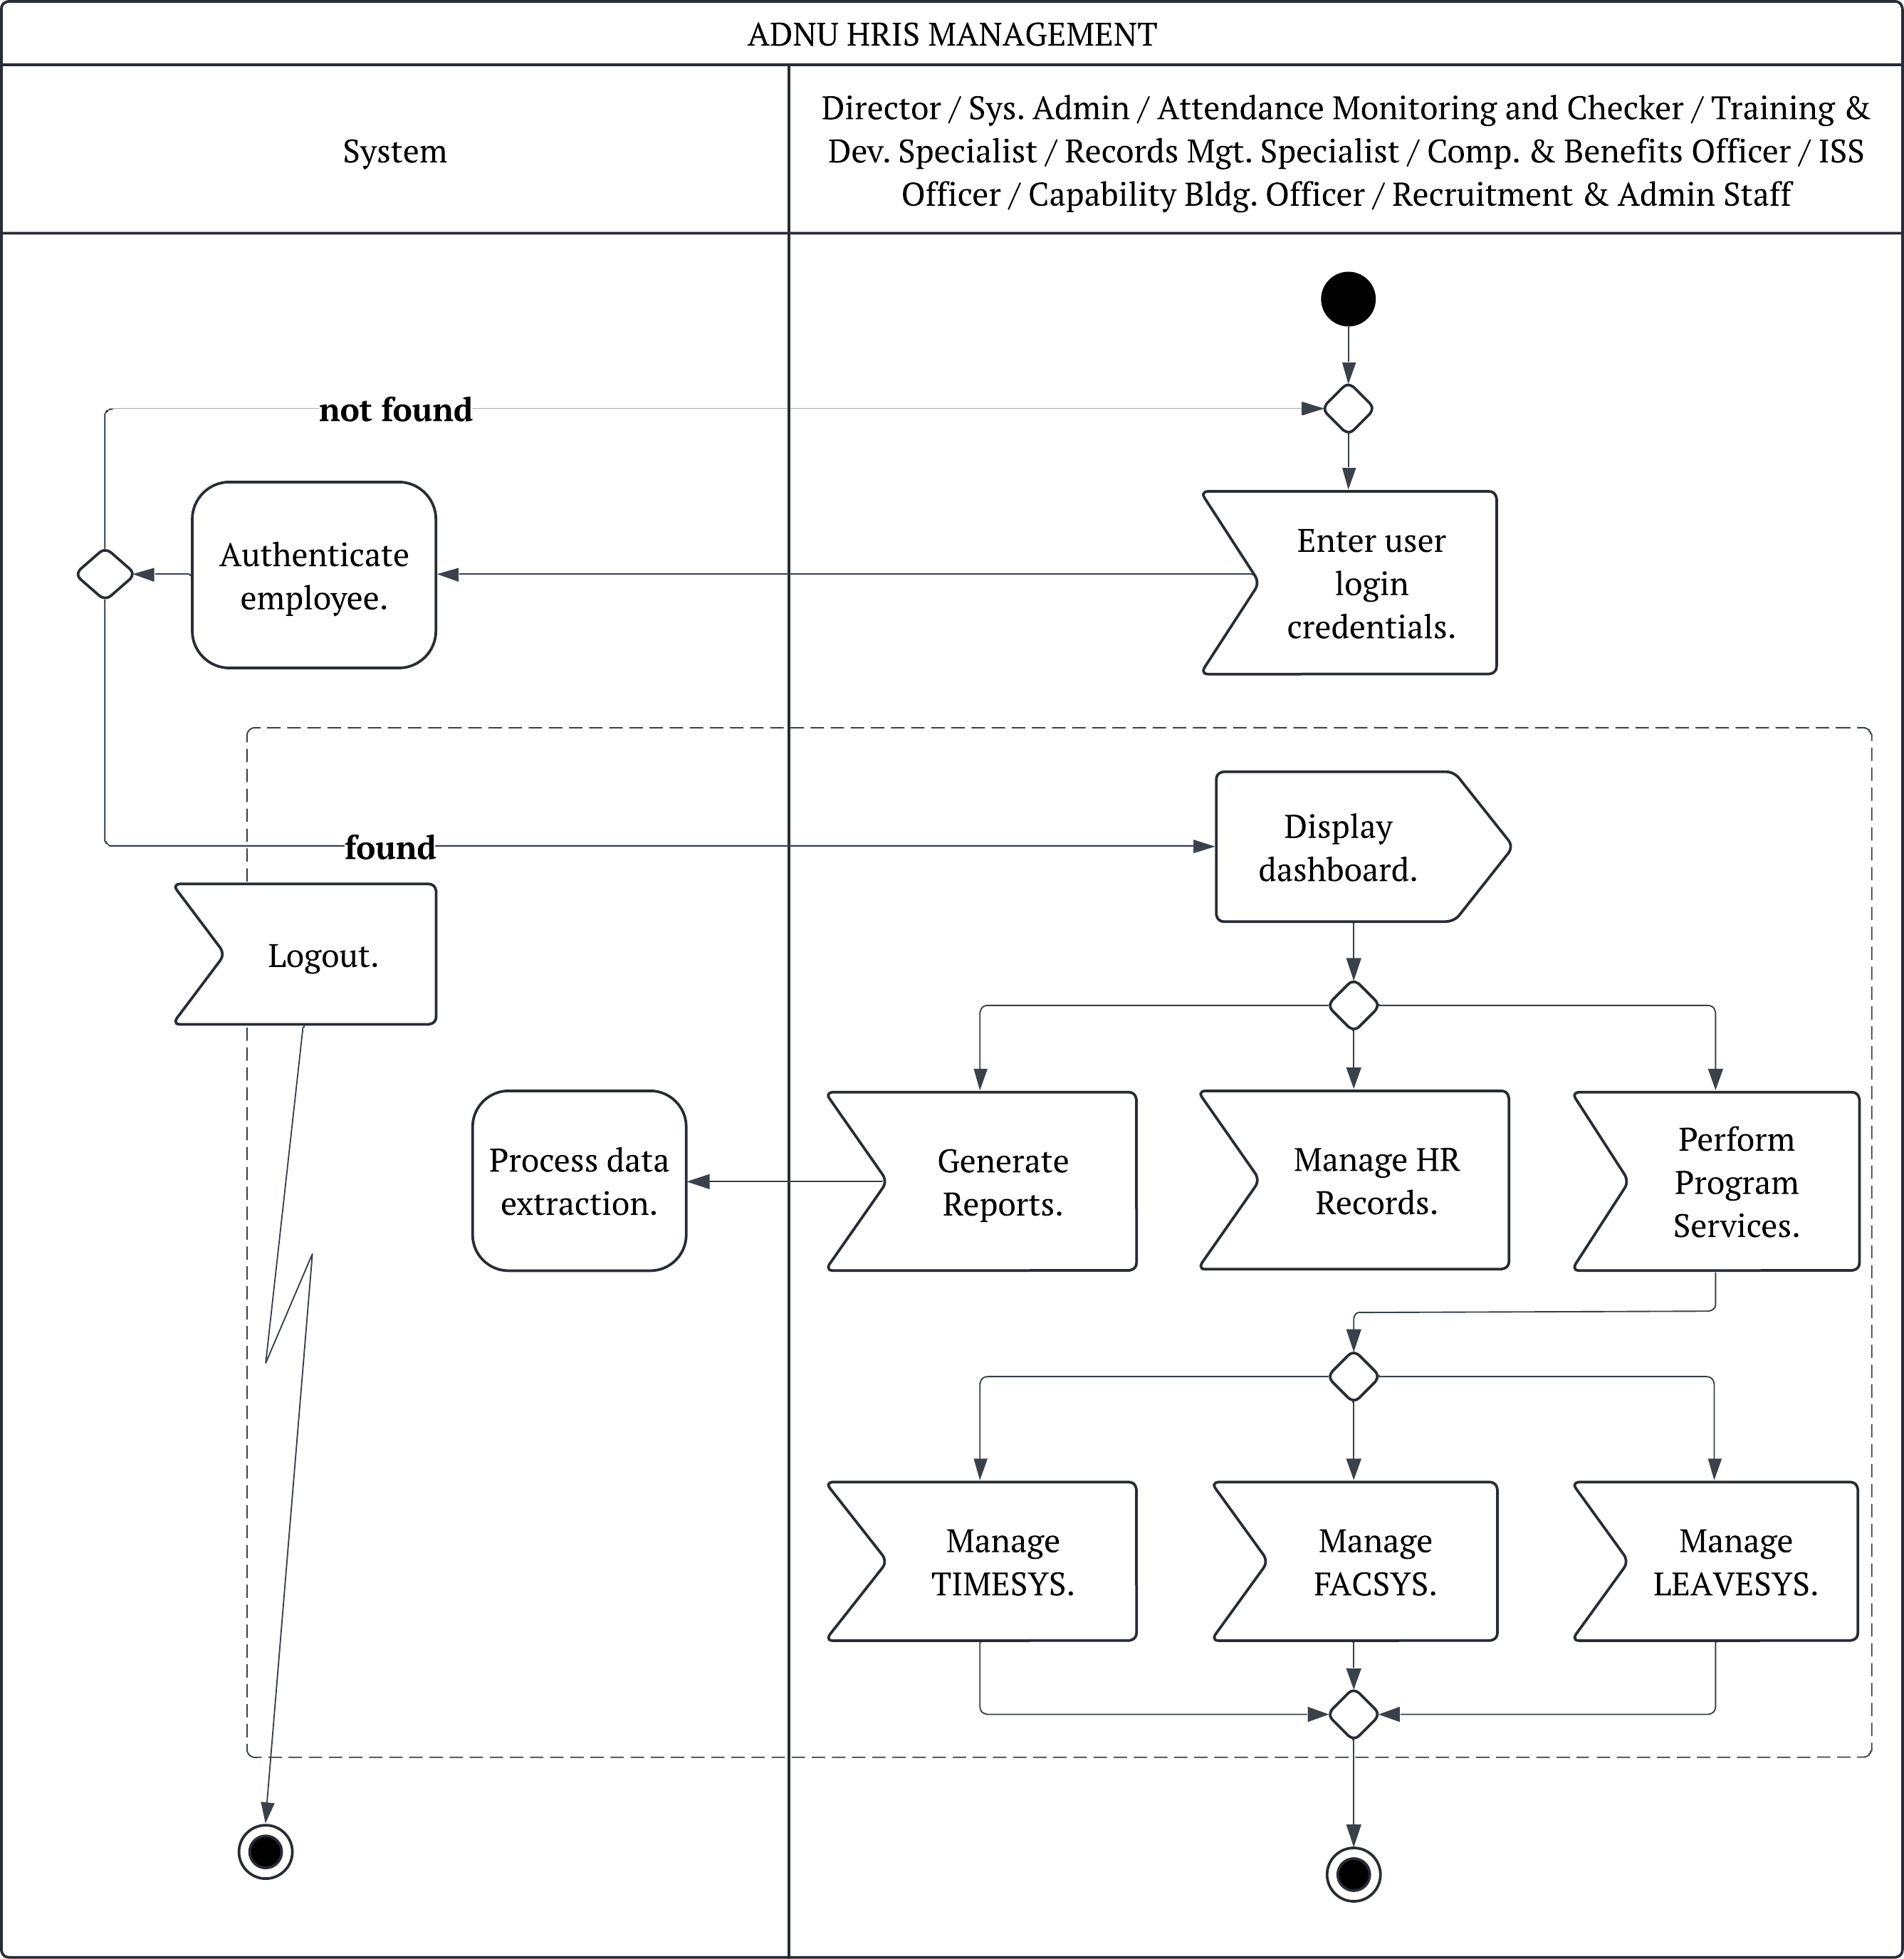
\includegraphics[width=1\linewidth]{figures/images/diagrams/swimlane/swimlane-admins.png}
        \caption{HRIS Swim-lane Diagram Model for HR Management.}
        \label{fig:swimlane-admins}
    \end{figure}

    Each role area can perform admin privileges and manage different modules within the system. For these actions, they are processed and managed under the system to provide a streamlined operation for any users in the system. Higher admins will have access to core modules e.g., Manage employee/personnel containing the employee contacts, personal information, profiles, assignments, assignment archive, faculty rank, academic, academic awards, professional license, training attendance, Certificate of Employment (COE), and health record.

    Besides this, these admins can also generate different kinds of reports within the system e.g., performing data extraction, queries, employee performance evaluation, COE reports, contracts/appointment generation, etc.

    \begin{figure}[H]
        \centering
        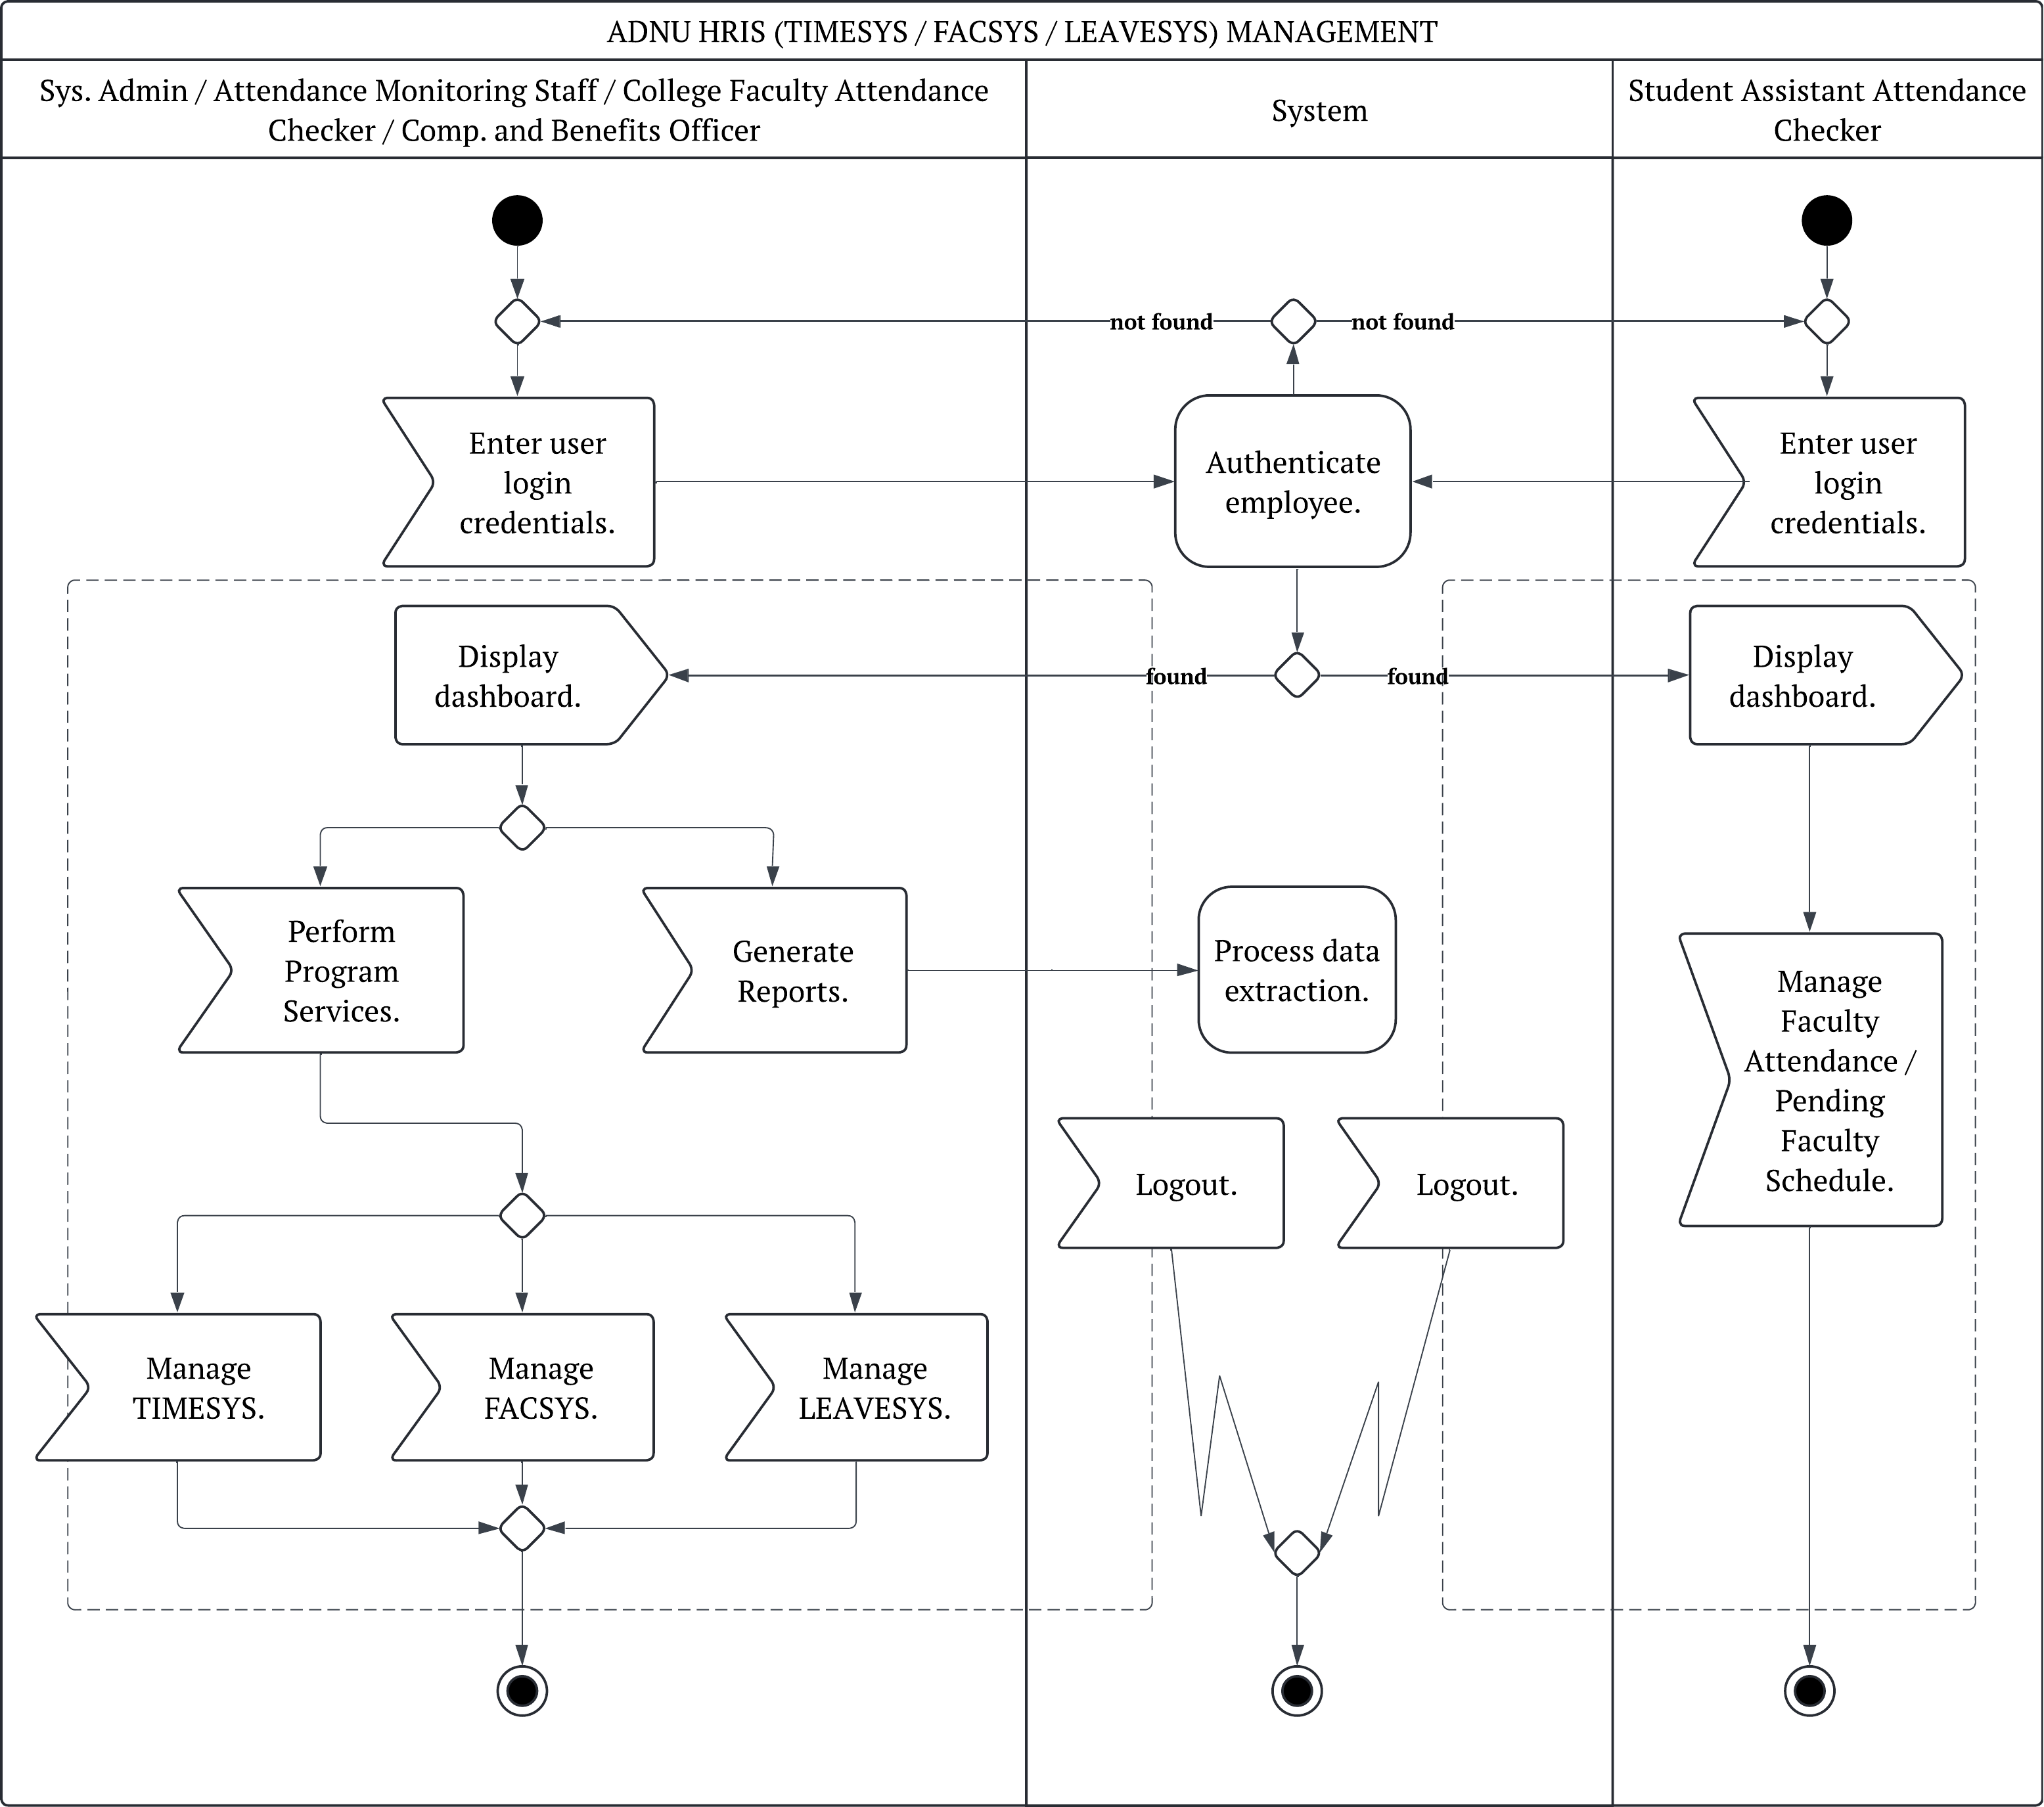
\includegraphics[width=1\linewidth]{figures/images/diagrams/swimlane/swimlane-sys-mgt.png}
        \caption{HRIS Swim-lane Diagram Model for TIMESYS, FACSYS, and LEAVESYS Management.}
        \label{fig:swimlane-sys-mgt}
    \end{figure}

    The system also includes modules for TIMESYS, FACSYS, and LEAVESYS. These modules are designed to manage employee attendance, faculty attendance, and employee leave applications, respectively. In the diagram, the identified roles along with their privilege are assigned to manage the three (3) SYS as well as allowing them to generate reports. Meanwhile, the Student Assistant Attendance Checker has lesser privilege and is assigned only to managing faculty attendance, faculty schedule, and managing pending faculty schedules.

    \subsection{Use Case Diagram}
    
    The use case diagram serves as a visual representation of the functional requirements of the system from an external user's perspective. It illustrates the interactions between users and the system, showcasing the various use cases and how they relate to each other. Each module referred to in \ref*{tab:hris-basic-modules}, \ref*{tab:hris-facsys-modules}, \ref*{tab:hris-leavesys-modules}, \ref*{tab:hris-timesys-modules} has specific use cases that define the functionalities and interactions within the system. Moreover, each module has different actors with specific roles and access levels, allowing for a comprehensive overview of the system's behavior and user interactions.
    
    Additionally, the concept of 'Manage' refers to the access users have to create, view, edit, and archive data or information within specific modules, By mapping out these interactions and incorporating both 'Manage' and 'View' functionalities, the use case diagram helps in identifying the system's behavior and the roles of different users in the HRIS application.

    In the HRIS Basic Modules Use Case Diagram, alongside Performing Data Extraction and Managing/Viewing Performance Evaluation, the use cases are grouped into four primary functional areas: Employee Information Access, Employment and Assignment Access, Academic and Professional Development Access, and Certification and Reporting Access. Each area extends to specific management or viewing capabilities. Employee Information Access covers personal data, profiles, health records, and professional licenses. Employment and Assignment Access encompasses employee assignments, their archives, and status information. Academic and Professional Development Access includes academic records, awards, and attended training sessions. Lastly, Certification and Reporting Access handles COE (Certificate of Employment) requests, reports, and contracts/appointments generation. This structure allows for efficient organization of various HRIS functions, providing comprehensive coverage of employee-related data management and access across different aspects of human resource operations.

    \begin{figure}[H]
        \centering
        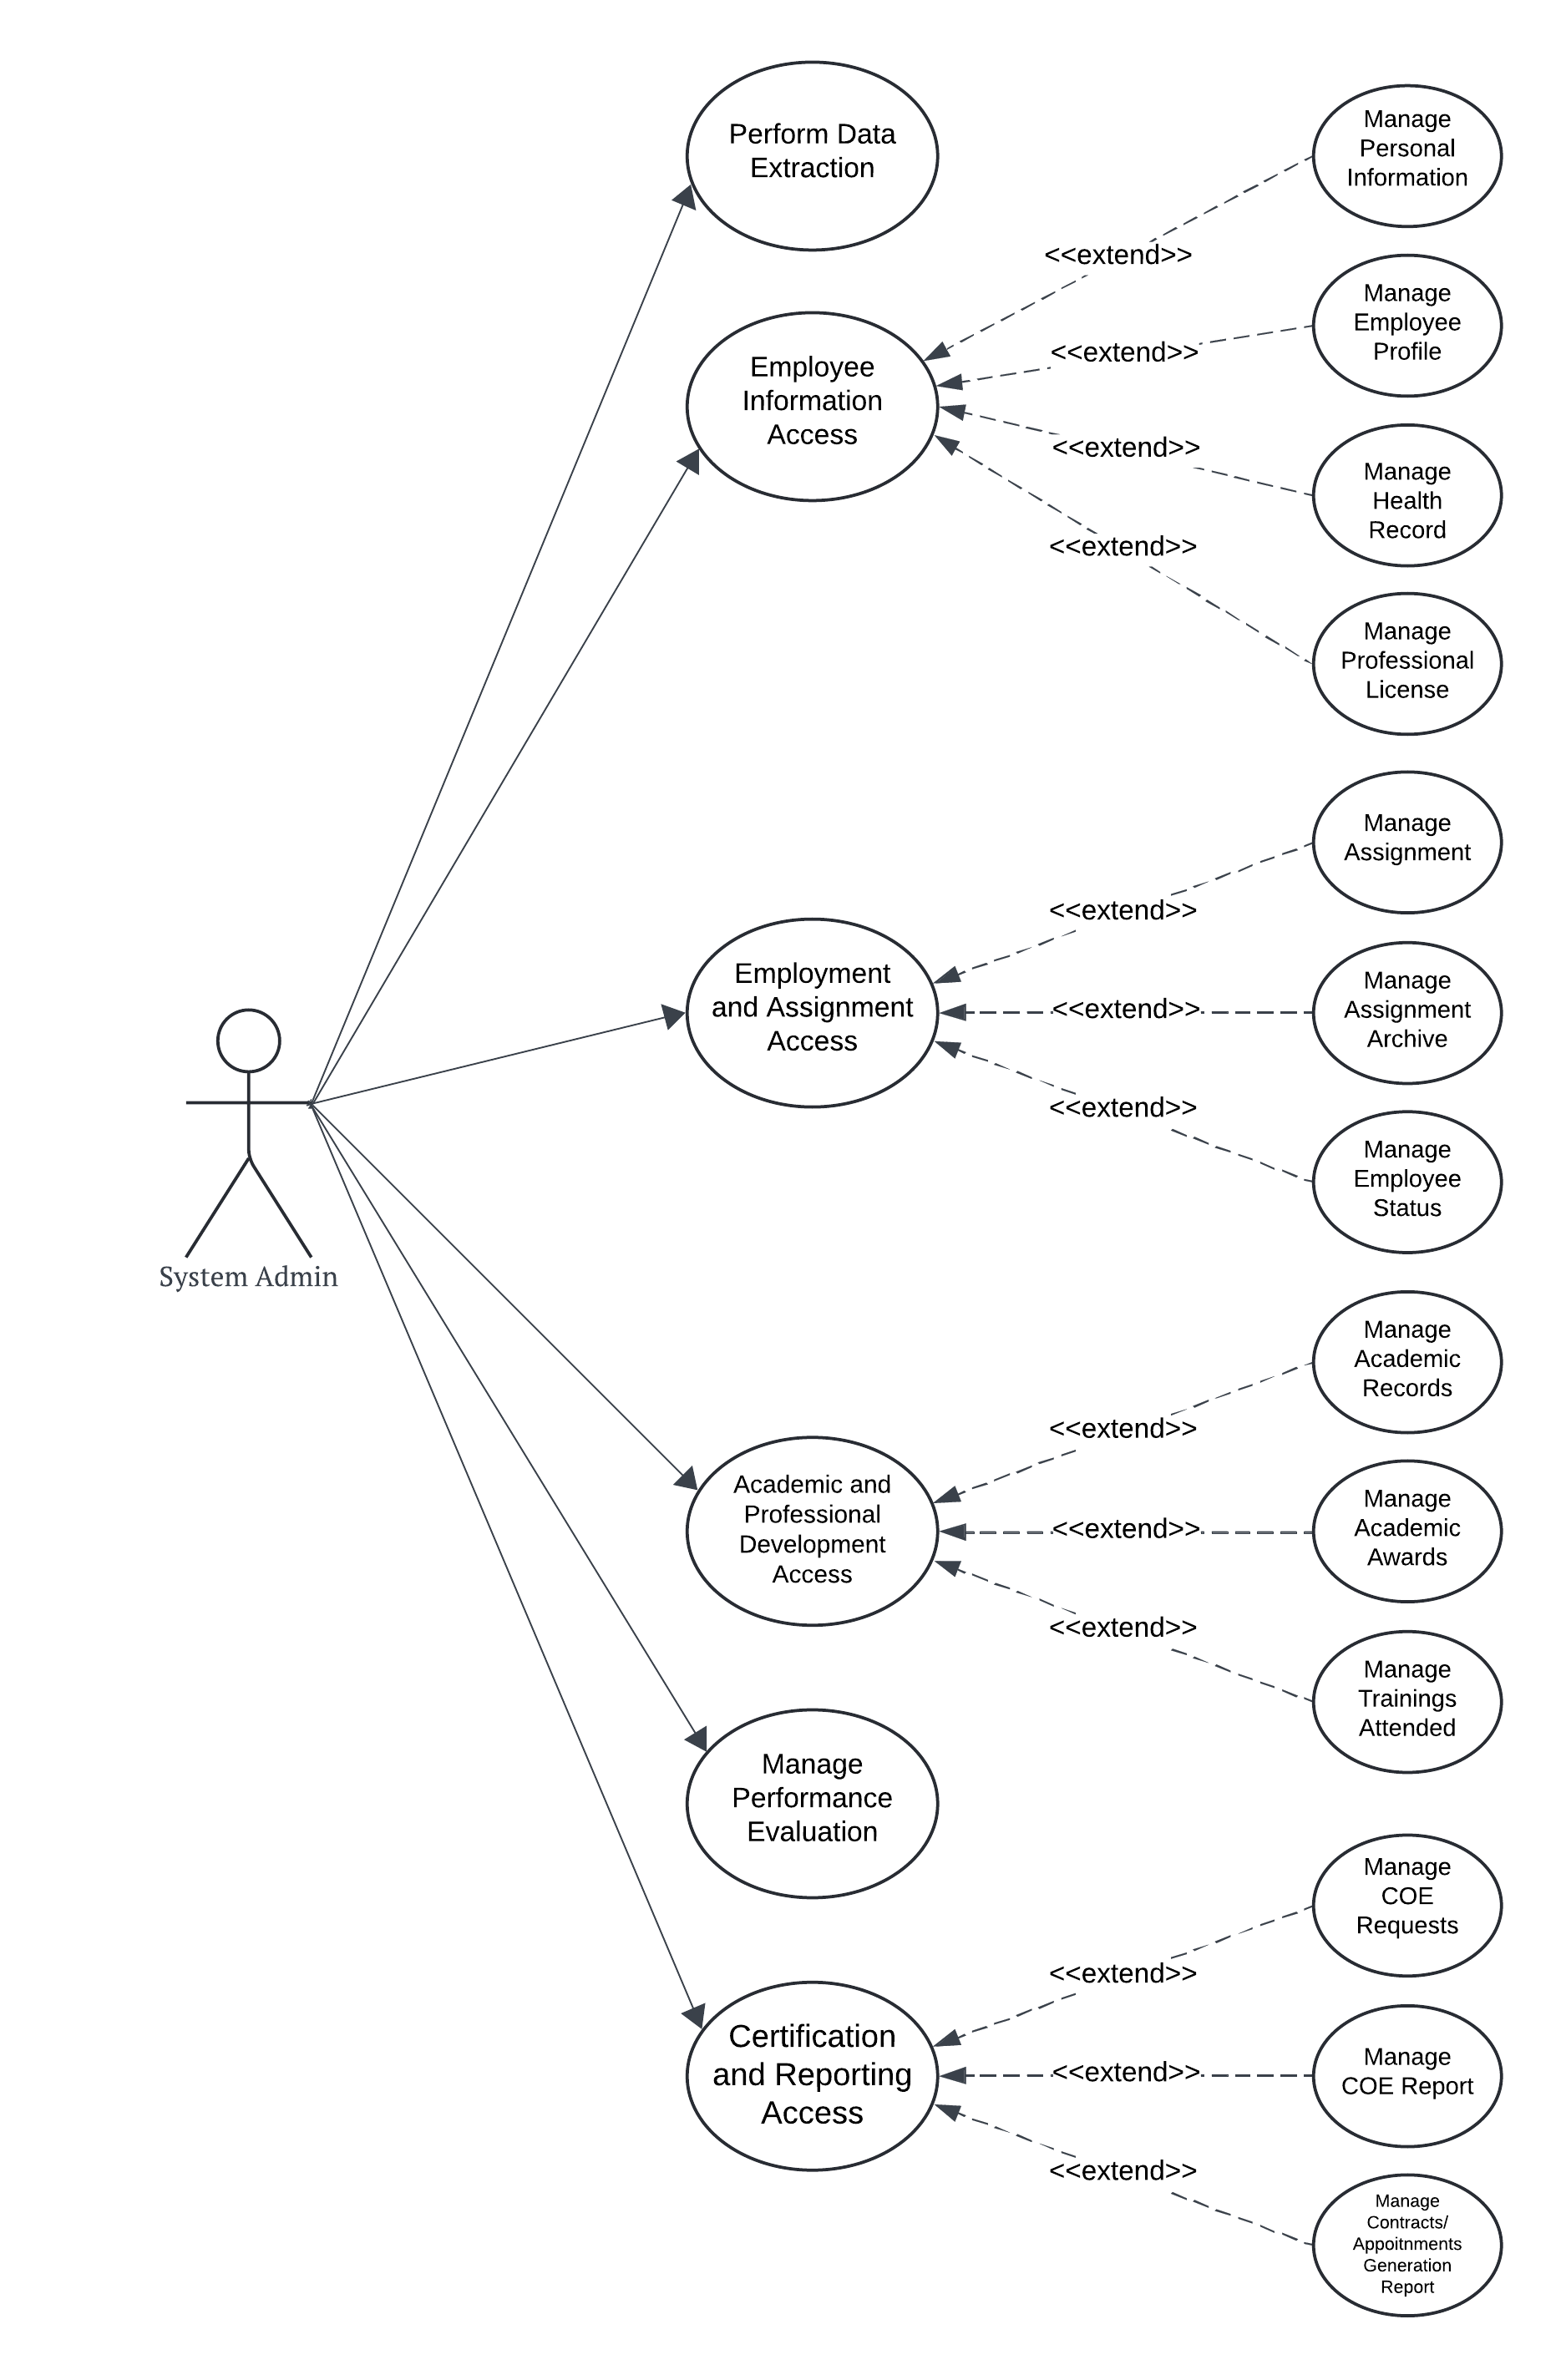
\includegraphics[width=0.9\linewidth]{figures/images/diagrams/usecase/use-case-basic-1.png}
        \caption{HRIS Basic Modules Use Case Diagram: System Admin.}
        \label{fig:use-case-basic-1}
    \end{figure}

    The figure \ref{fig:use-case-basic-1} shows the use case diagram for the System Admin within the HRIS Basic Modules. The System Admin has full managing access to all use cases. This includes Performing Data Extraction, Managing Performance Evaluation and all the modules that encompasses the 4 functional areas: Employee Information Access, Employment and Assignment Access, Academic and Professional Development Access, and Certification and Reporting Access. This comprehensive access enables the System Admin to oversee and manage all aspects of the HRIS application, ensuring efficient and effective HR operations.

    \begin{figure}[H]
        \centering
        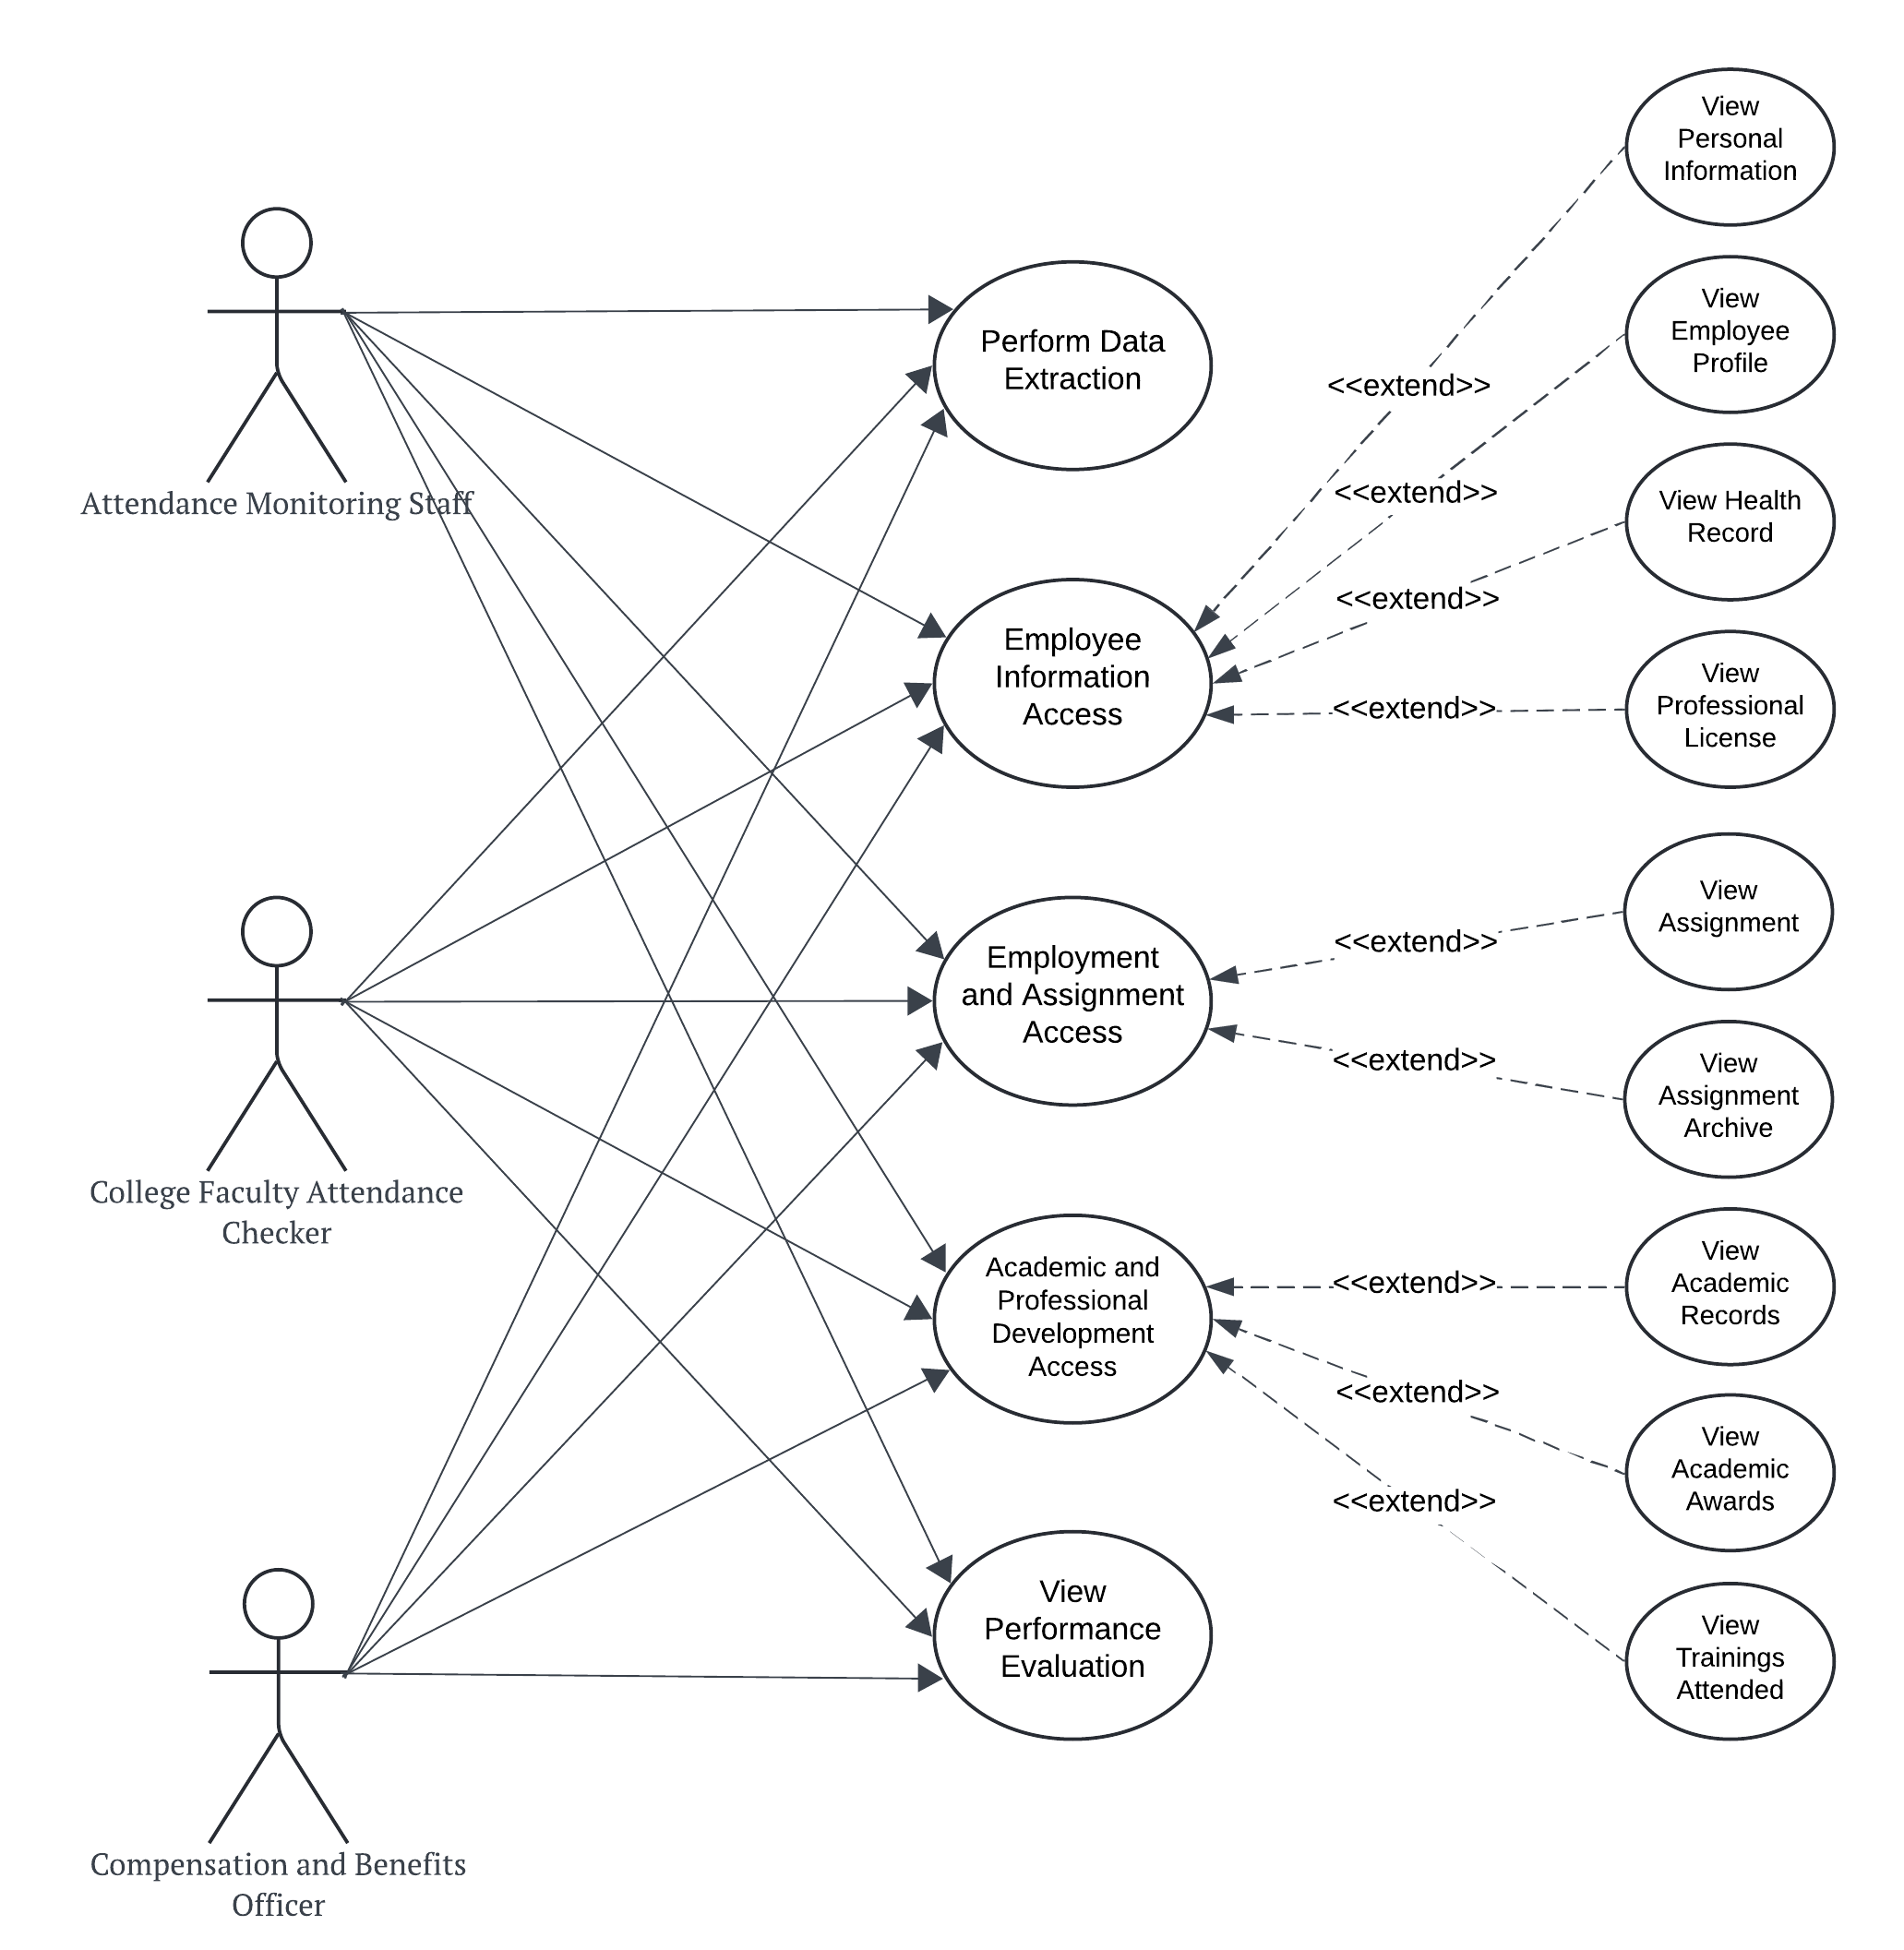
\includegraphics[width=0.9\linewidth]{figures/images/diagrams/usecase/use-case-basic-2.png}
        \caption{HRIS Basic Modules Use Case Diagram: Attendance Monitoring Staff, College Faculty Attendance Checker, and Compensation and Benefits Officer.}
        \label{fig:use-case-basic-2}
    \end{figure}

    The figure \ref{fig:use-case-basic-2} depicts the use case diagram for Attendance Monitoring Staff, College Faculty Attendance Checker, and Compensation and Benefits Officer within the HRIS Basic Modules. These three actors share identical access which is limited to view-only across most use cases. This includes Performing Data Extraction, Viewing Performance Evaluation, and all the use cases that encompasses the 3 functional areas: Employee Information Access, Employment and Assignment Access, and Academic and Professional Development Access. 

    \begin{figure}[H] 
        \centering
        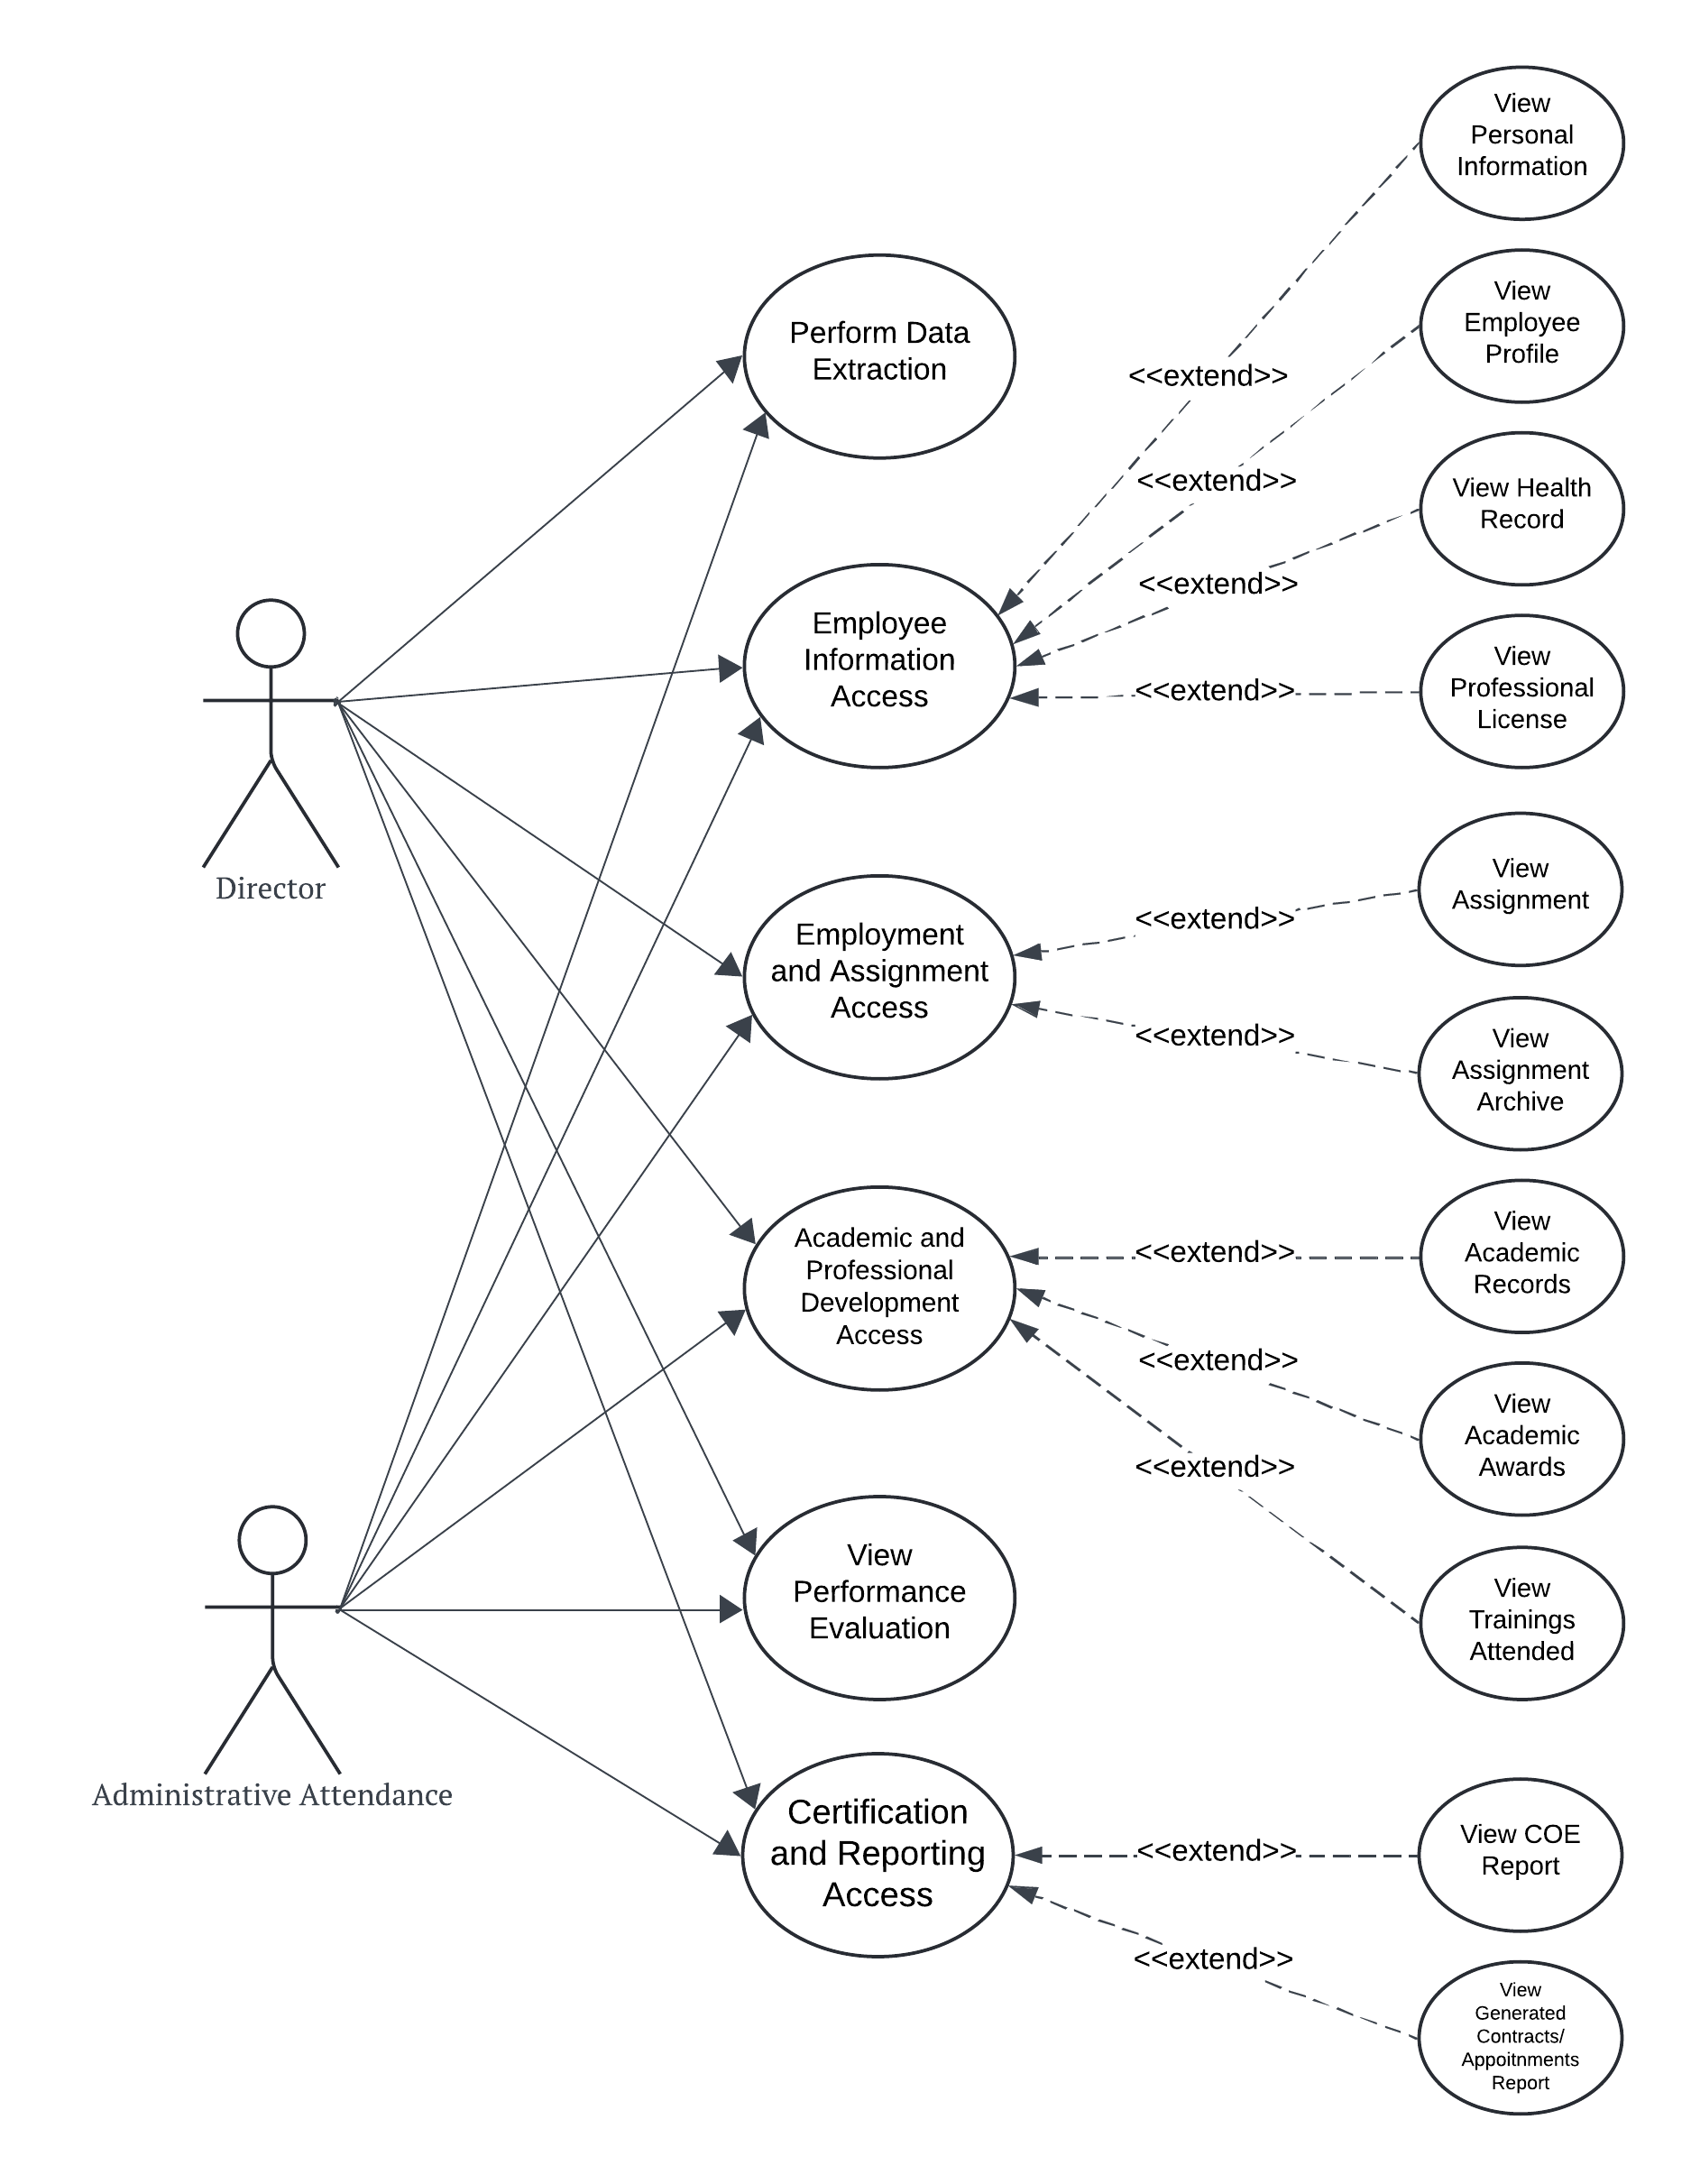
\includegraphics[width=0.9\linewidth]{figures/images/diagrams/usecase/use-case-basic-3.png}
        \caption{HRIS Basic Modules Use Case Diagram: Director and Administrative Assistant.}
        \label{fig:use-case-basic-3}
    \end{figure}

    The figure \ref{fig:use-case-basic-3} shows the use case diagram for the Director and Administrative Assistant within the HRIS Basic Modules. Both actors share access which is limited to view-only across all the use cases. This includes Performing Data Extraction, Viewing Performance Evaluation, and all the use cases that encompasses the 4 functional areas: Employee Information Access, Employment and Assignment Access, Academic and Professional Development Access, and Certification and Reporting Access. 

    \begin{figure}[H]
        \centering
        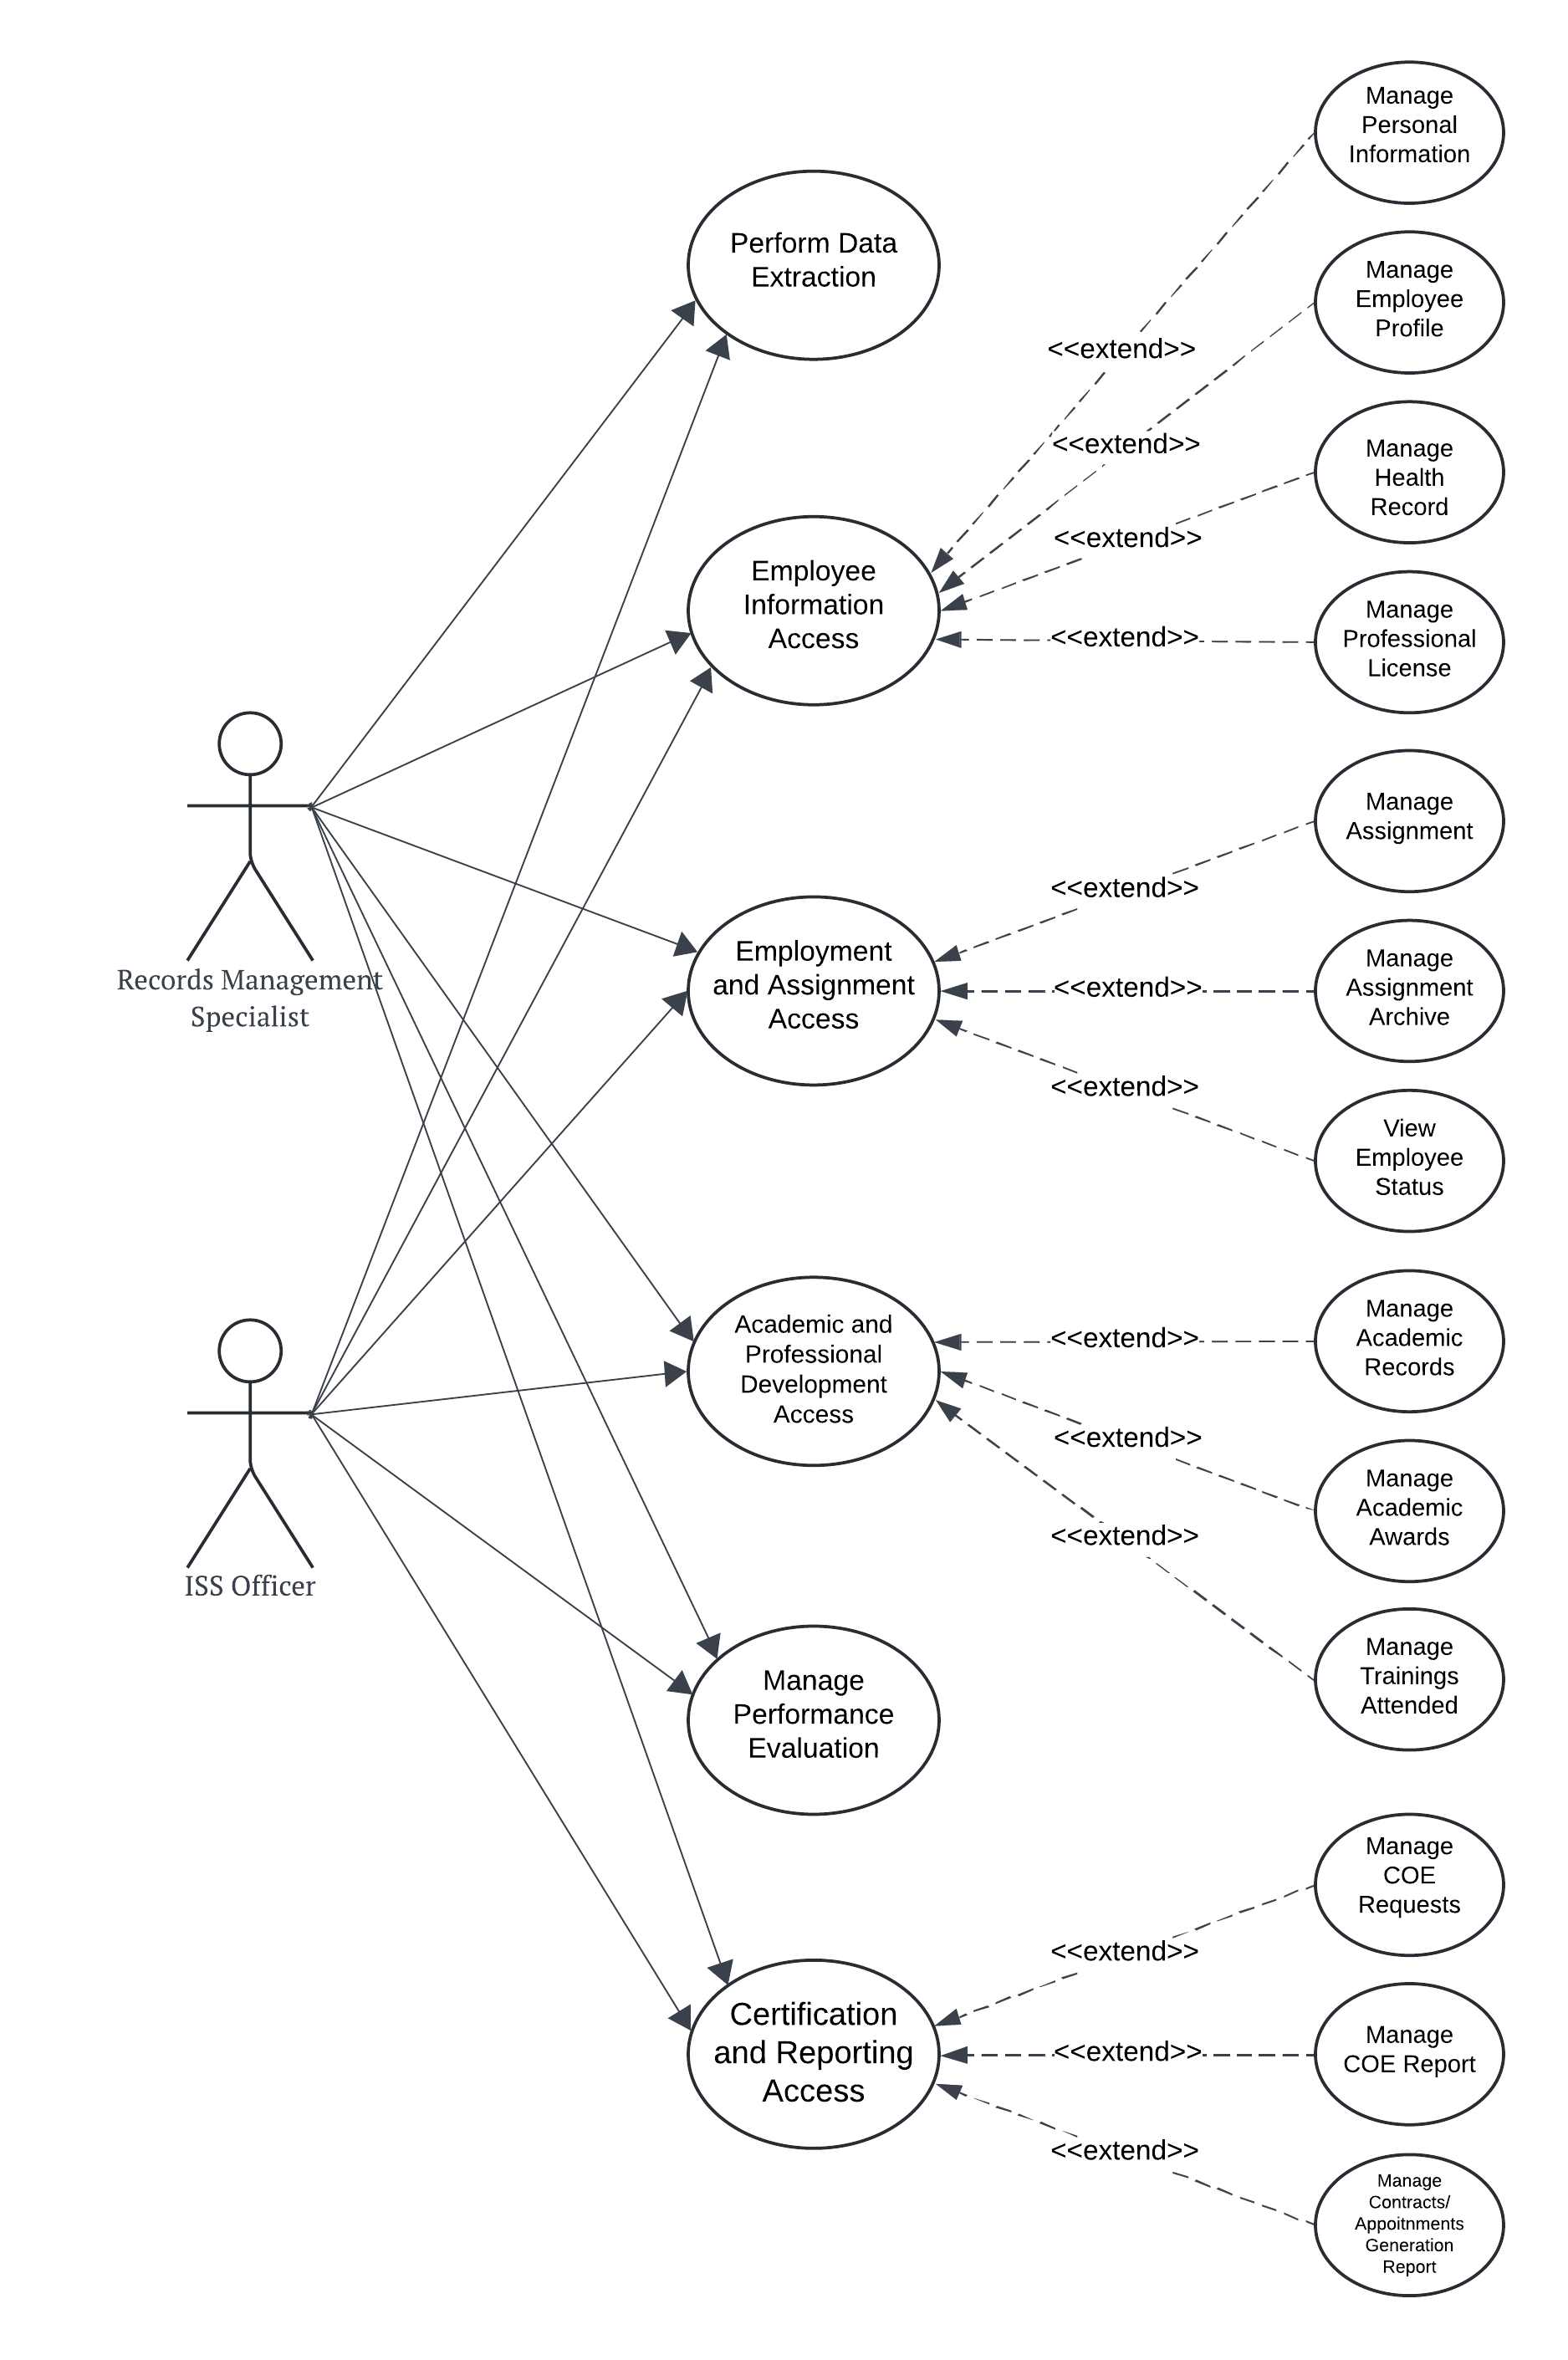
\includegraphics[width=0.9\linewidth]{figures/images/diagrams/usecase/use-case-basic-4.png}
        \caption{HRIS Basic Modules Use Case Diagram: Records Management Specialist and ISS Officer.}
        \label{fig:use-case-basic-4}
    \end{figure}

    The figure \ref{fig:use-case-basic-4} illustrates the use case diagram for the Records Management Specialist and ISS Officer.Both actors share the same access to the HRIS Basic Modules which is managing access to all use cases except one. This includes Performing Data Extraction, Managing Performance Evaluation, and all the use cases that encompasses the 4 functional areas: Employee Information Access, Employment and Assignment Access, Academic and Professional Development Access, and Certification and Reporting Access. The only exception is that, both actors can only view the employee status found in the Employment and Assignment Access functional area.

    \begin{figure}[H]
        \centering
        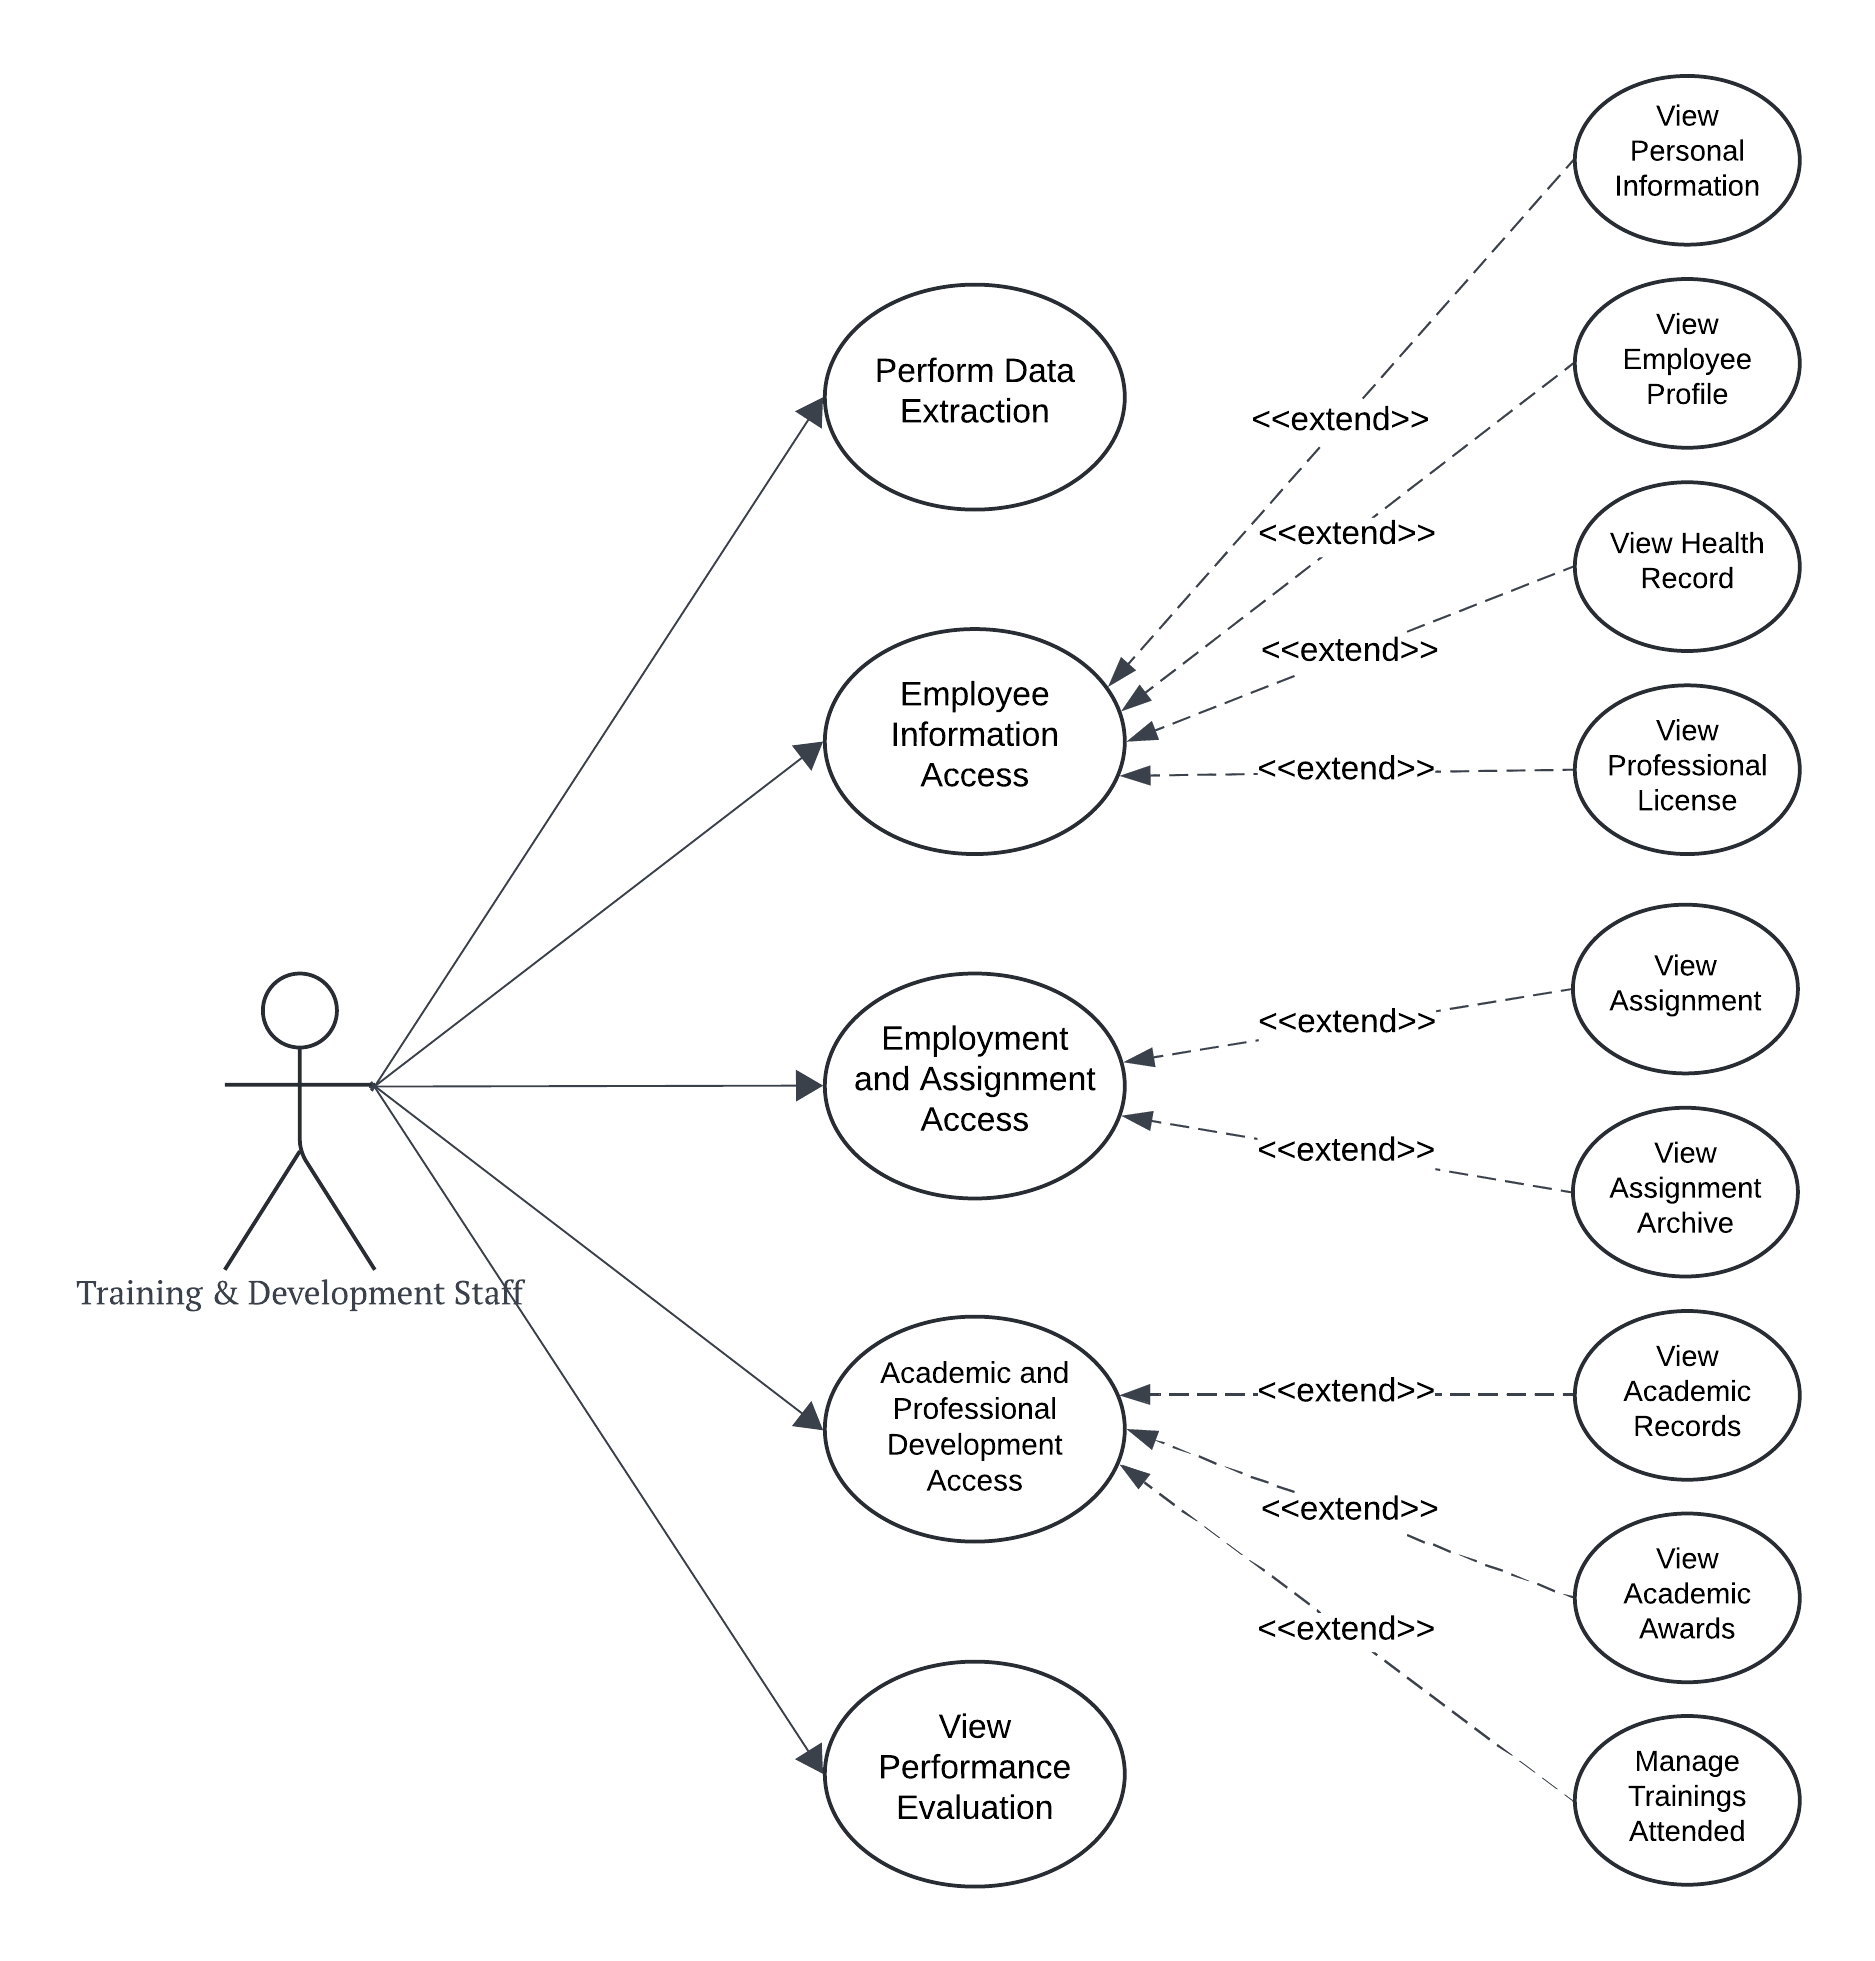
\includegraphics[width=0.9\linewidth]{figures/images/diagrams/usecase/use-case-basic-5.png}
        \caption{HRIS Basic Modules Use Case Diagram: Training and Development Staff.}
        \label{fig:use-case-basic-5}
    \end{figure}
    
    The figure \ref{fig:use-case-basic-5} demonstrates the use case diagram for the Training and Development Staff within the HRIS Basic Modules. The actor has limited view access to the most of the use cases. This includes Performing Data Extraction, Viewing Performance Evaluation, and also the use cases that  encompasses the 3 functional areas: Employee Information Access, Employment and Assignment Access, and Academic and Professional Development Access. The only exception is that, the Training and Development Staff has the privilege to Manage the Trainings Attended of the employees found in the Academic and Professional Development Access functional area.

    \begin{figure}[H]
        \centering
        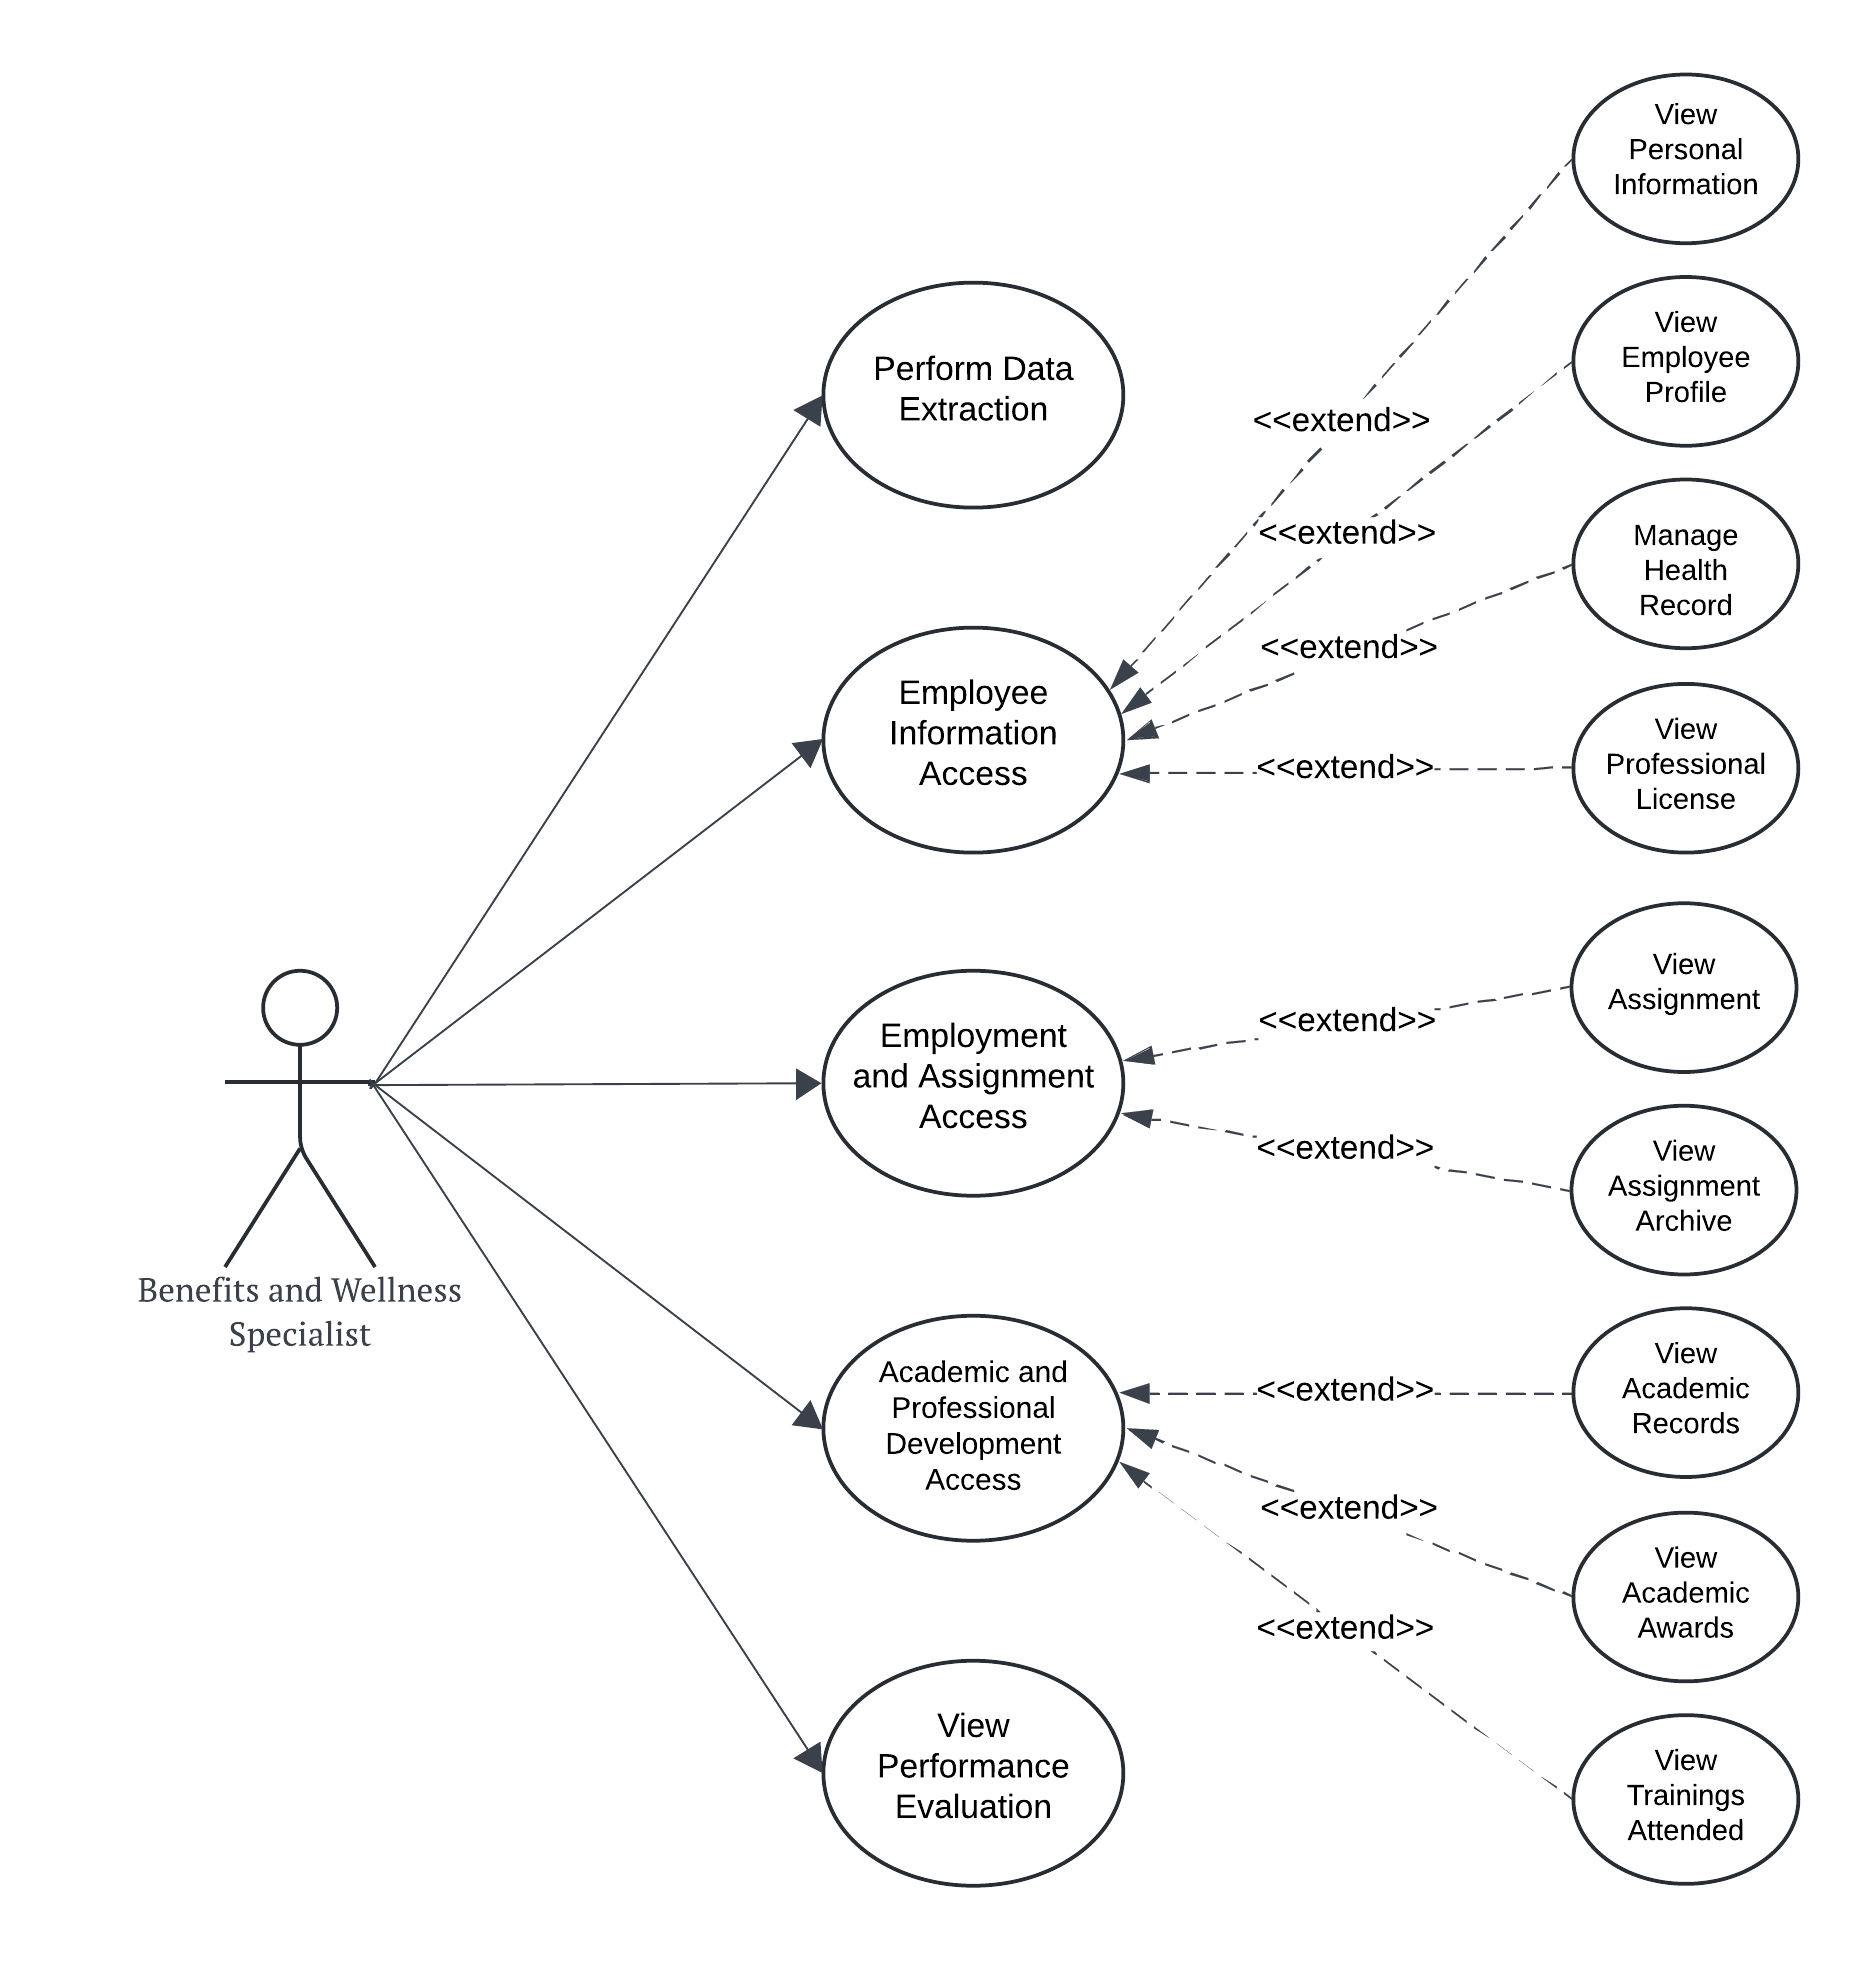
\includegraphics[width=0.9\linewidth]{figures/images/diagrams/usecase/use-case-basic-6.png}
        \caption{HRIS Basic Modules Use Case Diagram: Benefits and Wellness Specialist.}
        \label{fig:use-case-basic-6}
    \end{figure}

    The figure \ref{fig:use-case-basic-6} shows the use case diagram for Benefits and Wellness Specialist. The actor has limited view access to the most of the use cases within the HRIS Basic Modules. This includes Performing Data Extraction, Viewing Performance Evaluation, and also the use cases that  encompasses the 3 functional areas: Employee Information Access, Employment and Assignment Access, and Academic and Professional Development Access. The only exception is that, the Benefits and Wellness Specialist was able to Manage the Health Records of the employees which is found in the Employee Information Access functional area.

    \begin{figure}[H]
        \centering
        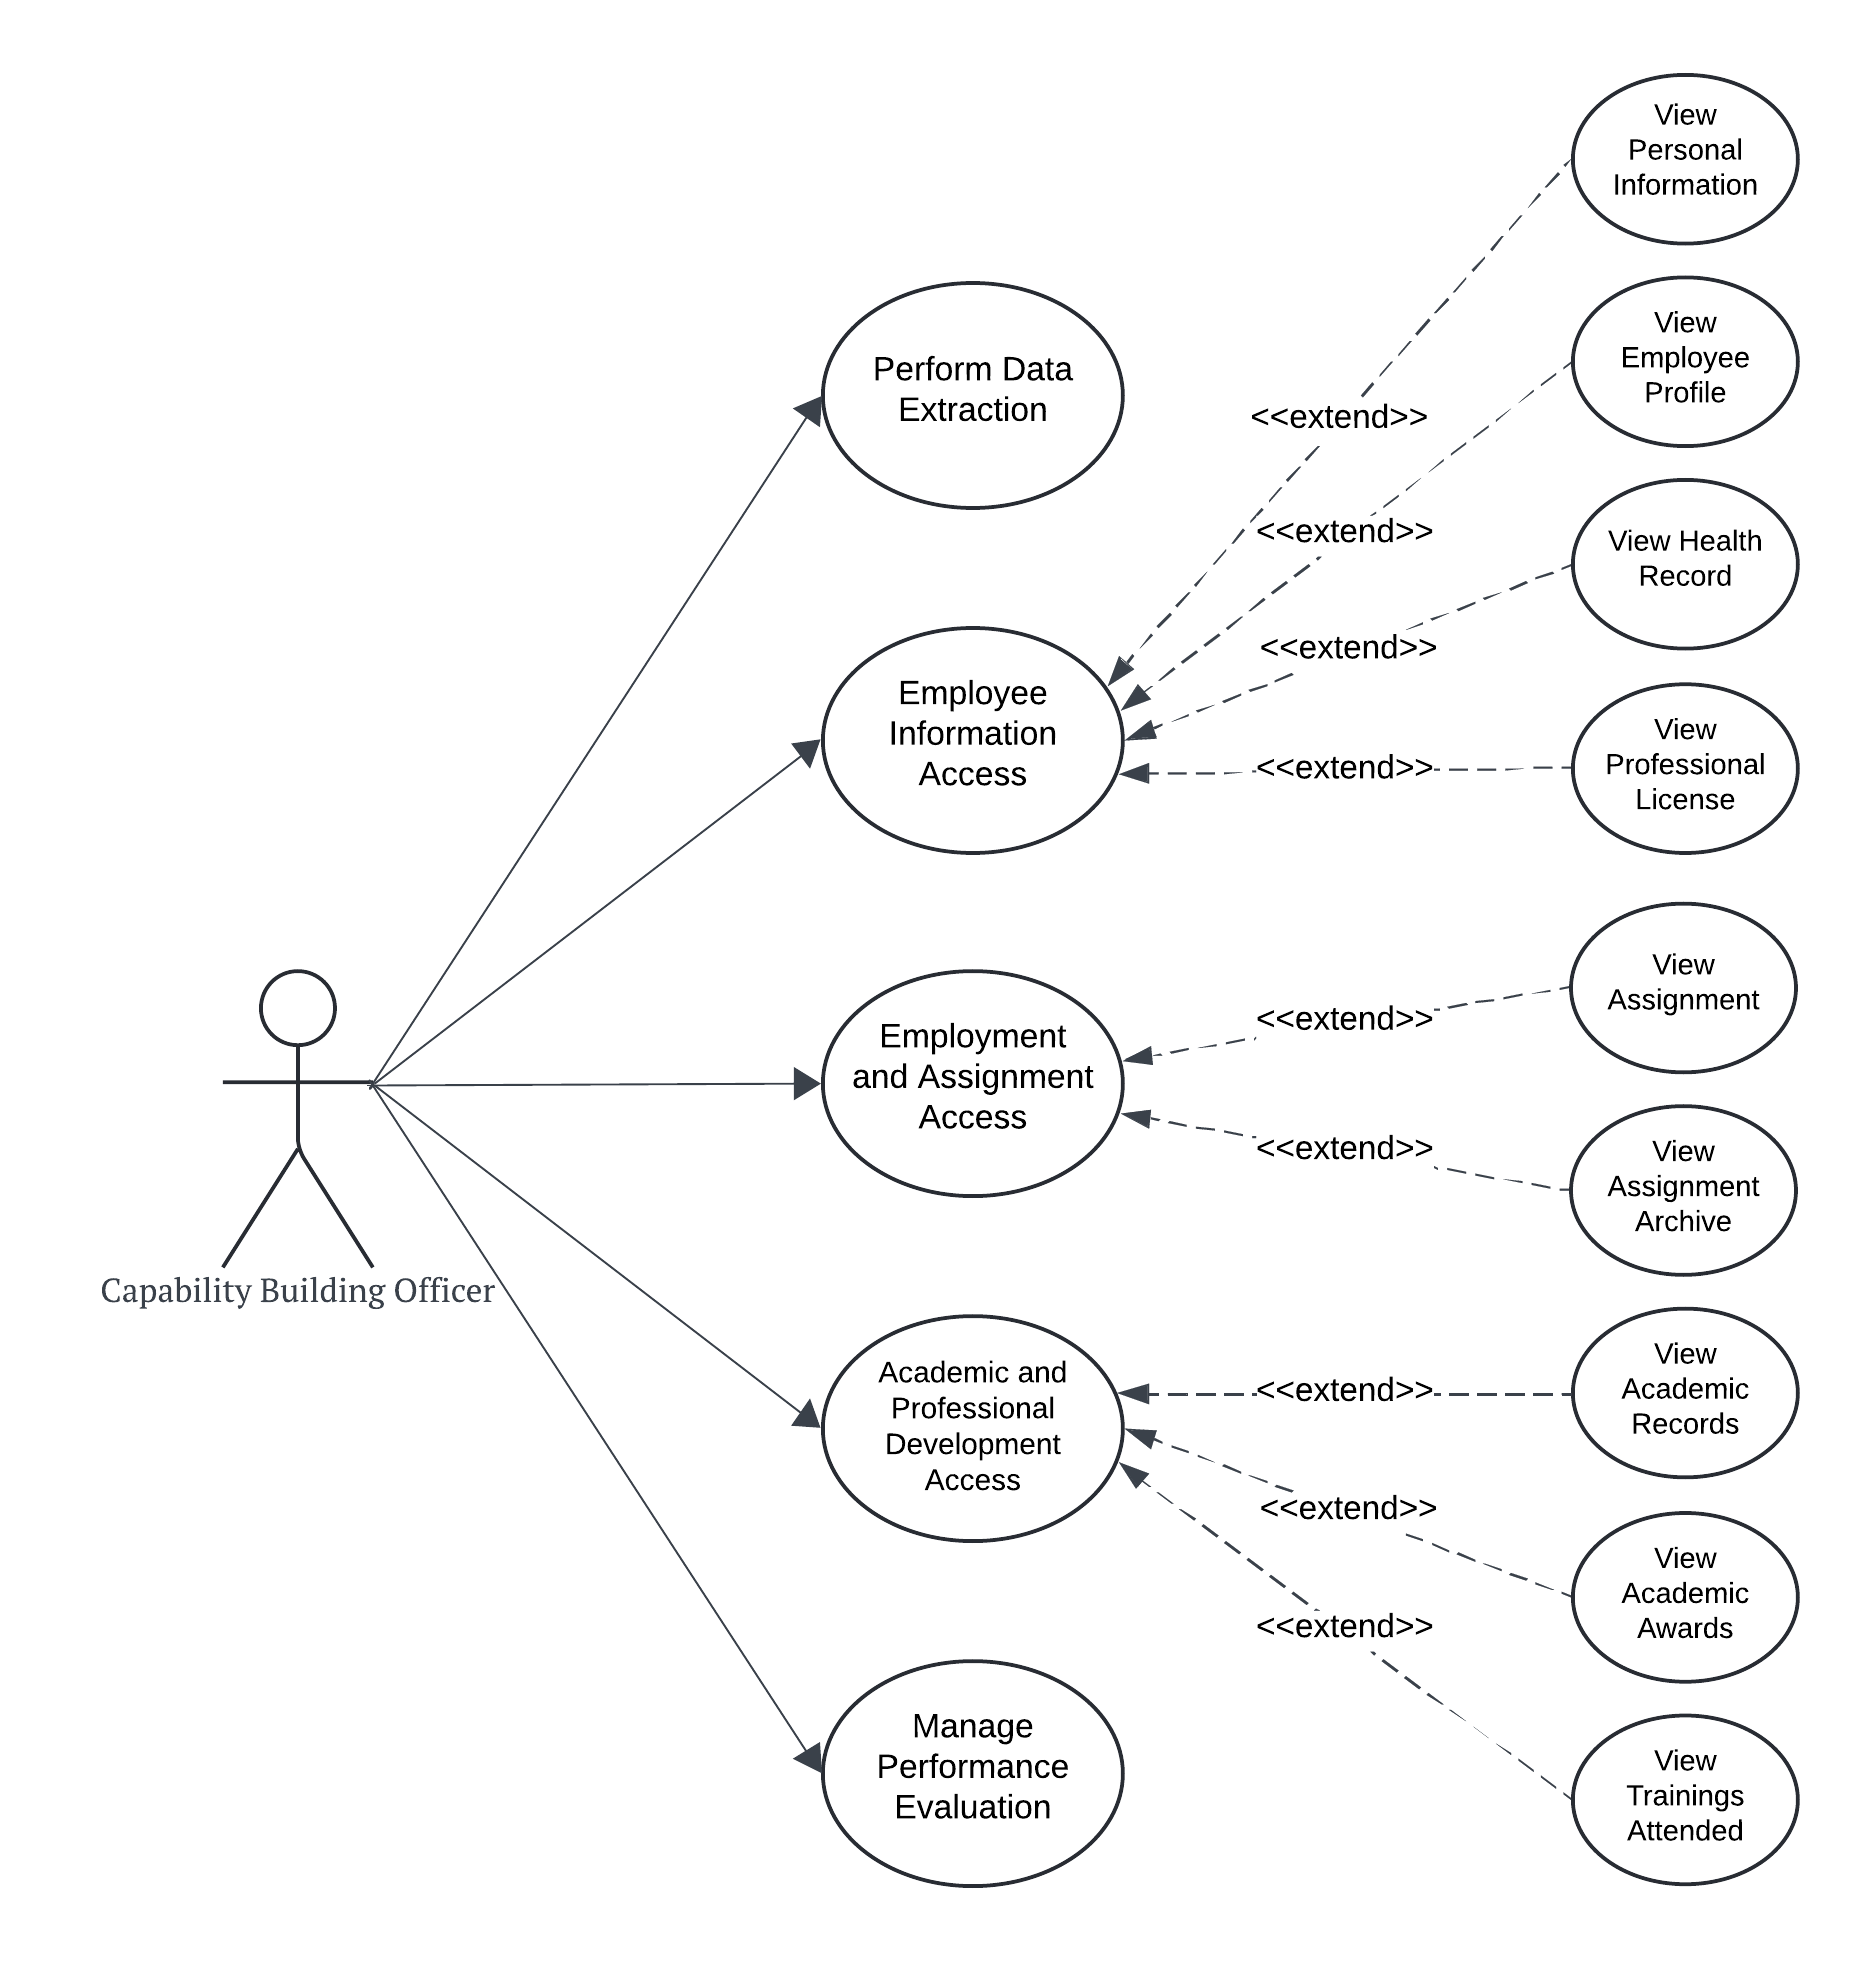
\includegraphics[width=0.9\linewidth]{figures/images/diagrams/usecase/use-case-basic-7.png}
        \caption{HRIS Basic Modules Use Case Diagram: Capability Building Officer.}
        \label{fig:use-case-basic-7}
    \end{figure}

    The figure \ref{fig:use-case-basic-7} illustrates the use case diagram for the Capability Building Officer. The actor has limited view access to the most of the use cases within the HRIS Basic Modules. This includes Performing Data Extraction, and the use cases that  encompasses the 3 functional areas: Employee Information Access, Employment and Assignment Access, and Academic and Professional Development Access. Moreover, the Capability Building Officer has the privilege to Manage the Performance Evaluation of the employees.

    \begin{figure}[H]
        \centering
        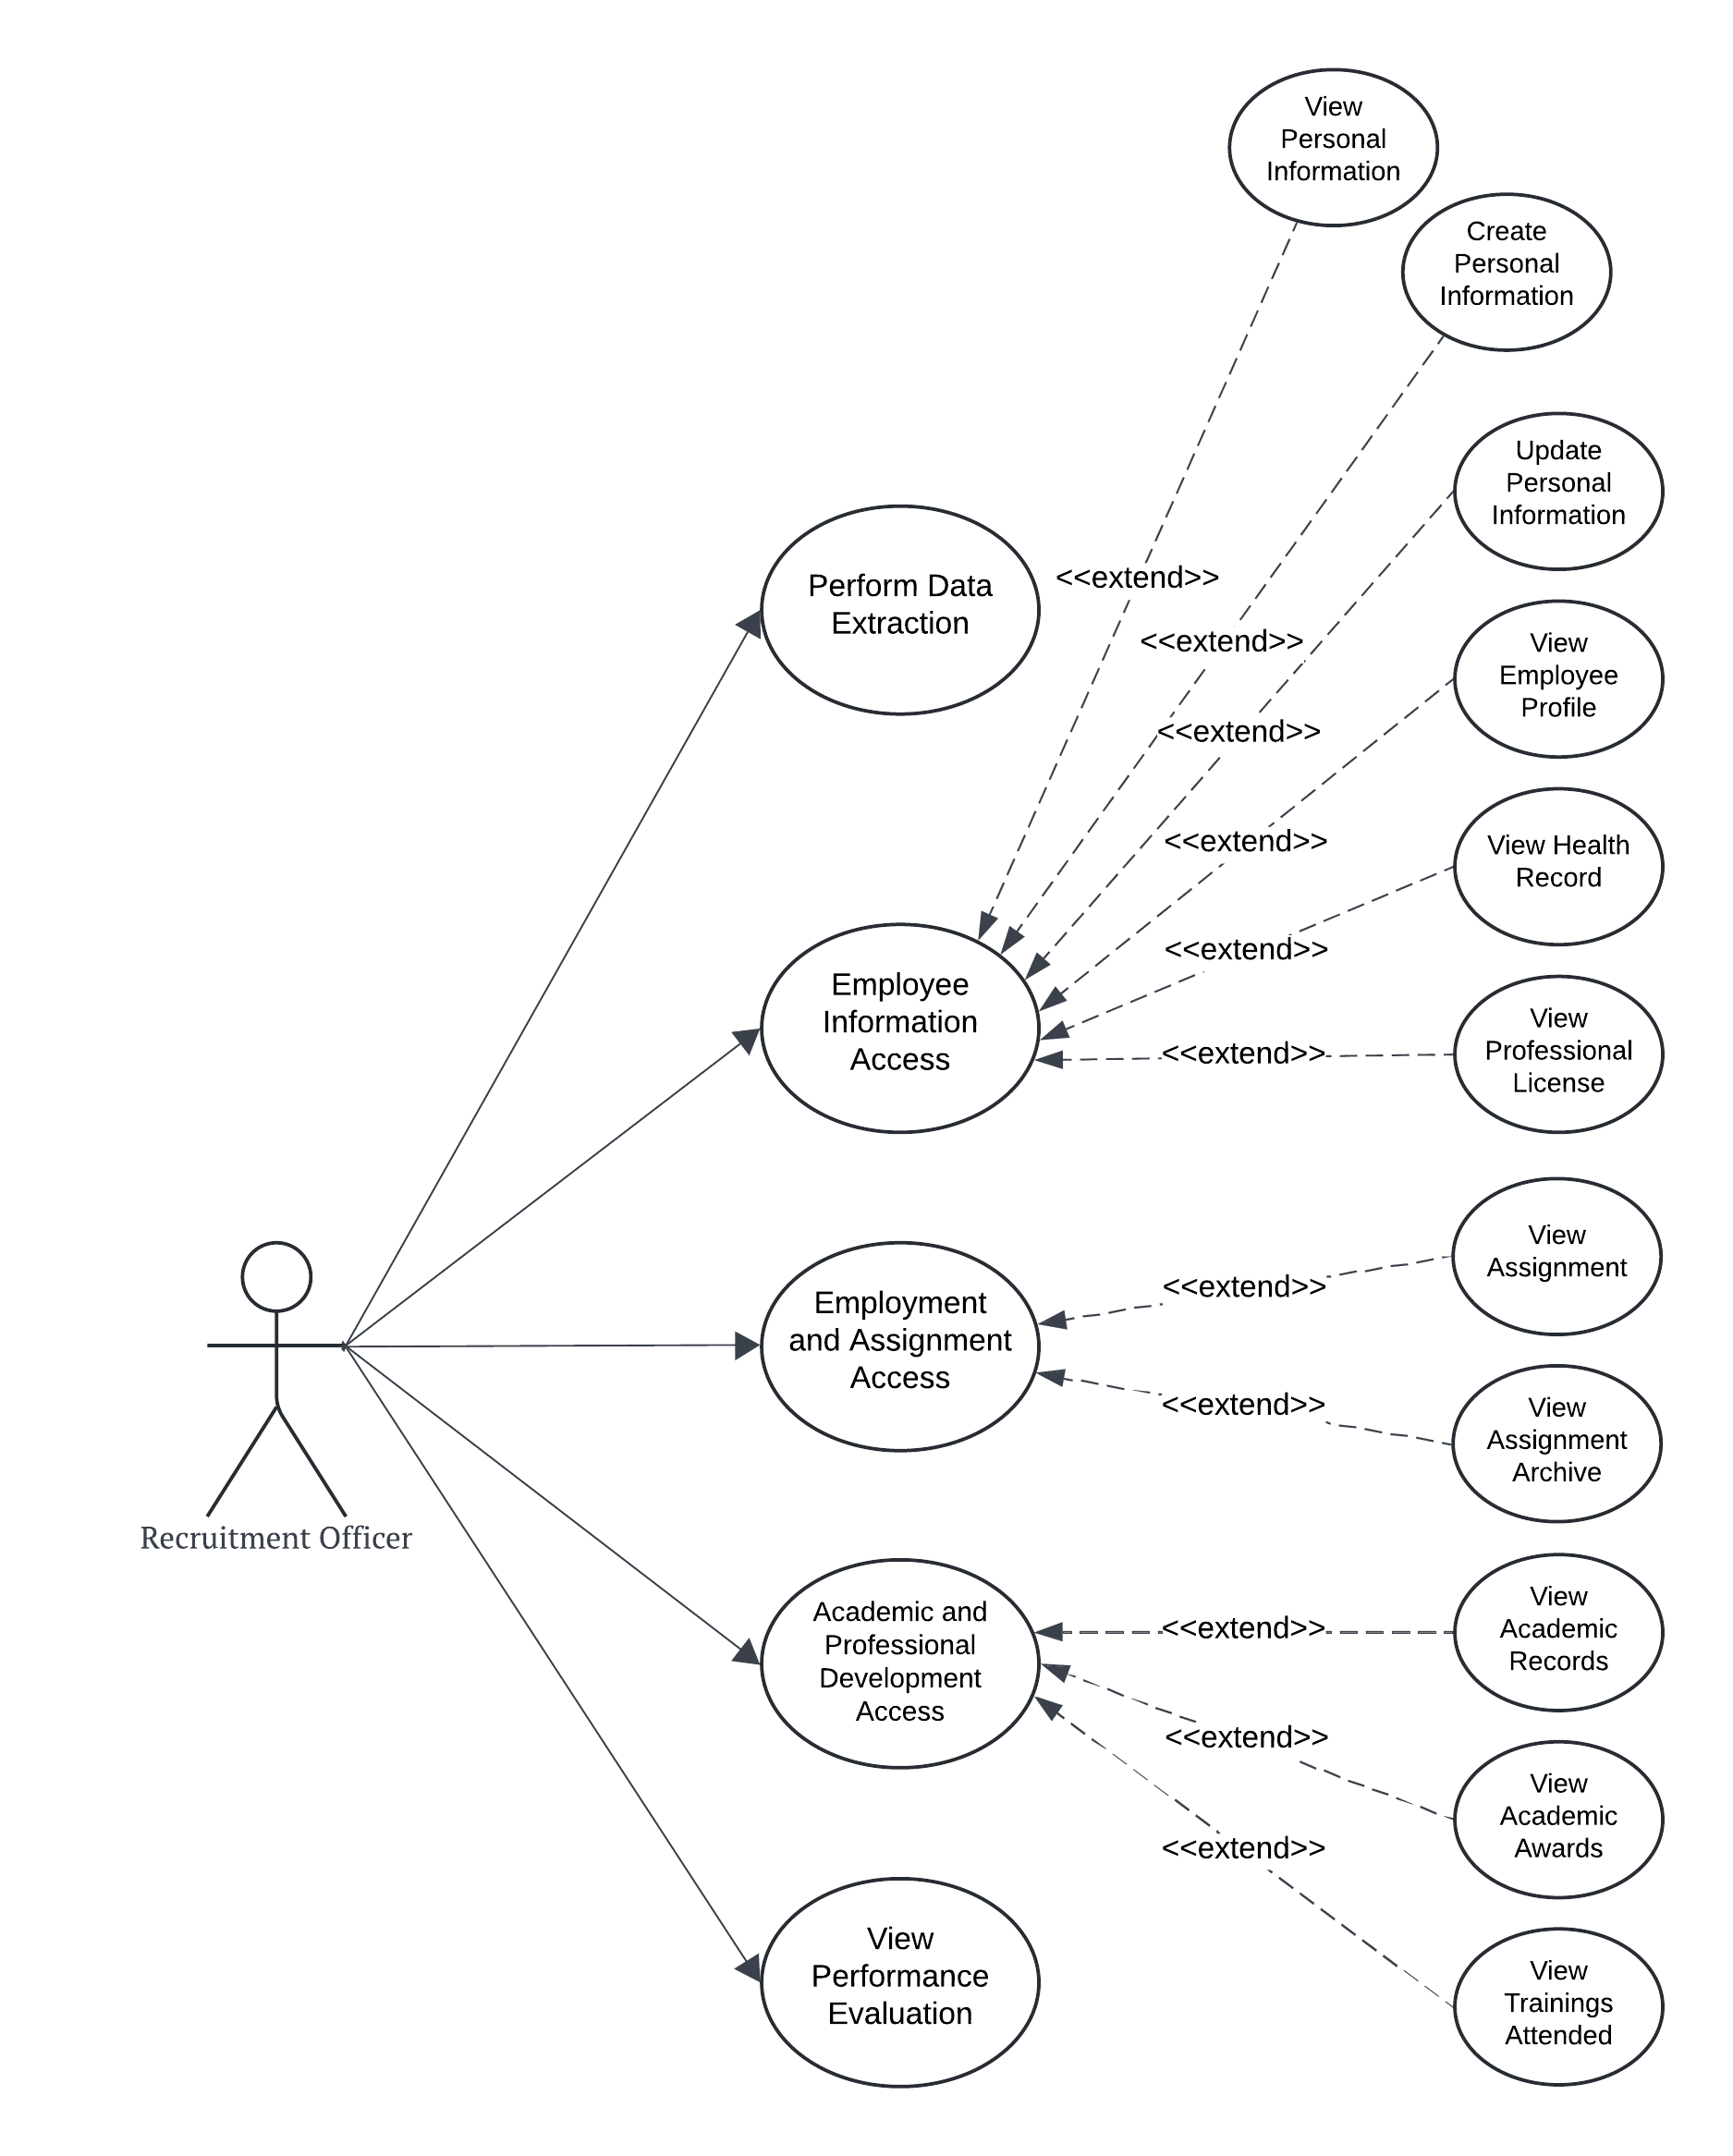
\includegraphics[width=0.9\linewidth]{figures/images/diagrams/usecase/use-case-basic-8.png}
        \caption{HRIS Basic Modules Use Case Diagram: Recruitment Officer.}
        \label{fig:use-case-basic-8}
    \end{figure}

    The figure \ref{fig:use-case-basic-8} illustrates the use case diagram for Recruitment Officers. The actor has limited view access to the most of the use cases within the HRIS Basic Modules. This includes Performing Data Extraction, Viewing Performance Evaluation, and the use cases that  encompasses the 3 functional areas: Employee Information Access, Employment and Assignment Access, and Academic and Professional Development Access. The only exception is that,  in the Employee Information Access functional area, the Recruitment Officer has a distinct privilege which is to view, create, and update the personal information of the employees.


    This section presents the use case diagram for the HRIS TIMESYS Module. The module involves four primary actors: System Admin, Attendance Monitoring Staff, College Faculty Attendance Checker, and Compensation and Benefits Officer. Each actor has specific access to various use cases within the TIMESYS module, enabling them to perform functions related to employee attendance monitoring and management.

    The module encompasses several key use cases, including managing employee attendance. This extends to archived attendance records and the generation of attendance reports. Additionally, it covers use cases related to managing work schedules, overtime, and holidays. A distinct functional area is created specifically for categorizing the management of tardiness, AWOL (Absent Without Leave), and remarks. This structured approach ensures comprehensive coverage of all time-related aspects of employee management.

    This diagram provides a comprehensive overview of the roles and responsibilities within the TIMESYS module, ensuring each actor has the necessary access to perform their tasks effectively.
    
    \begin{figure}[H]
        \centering
        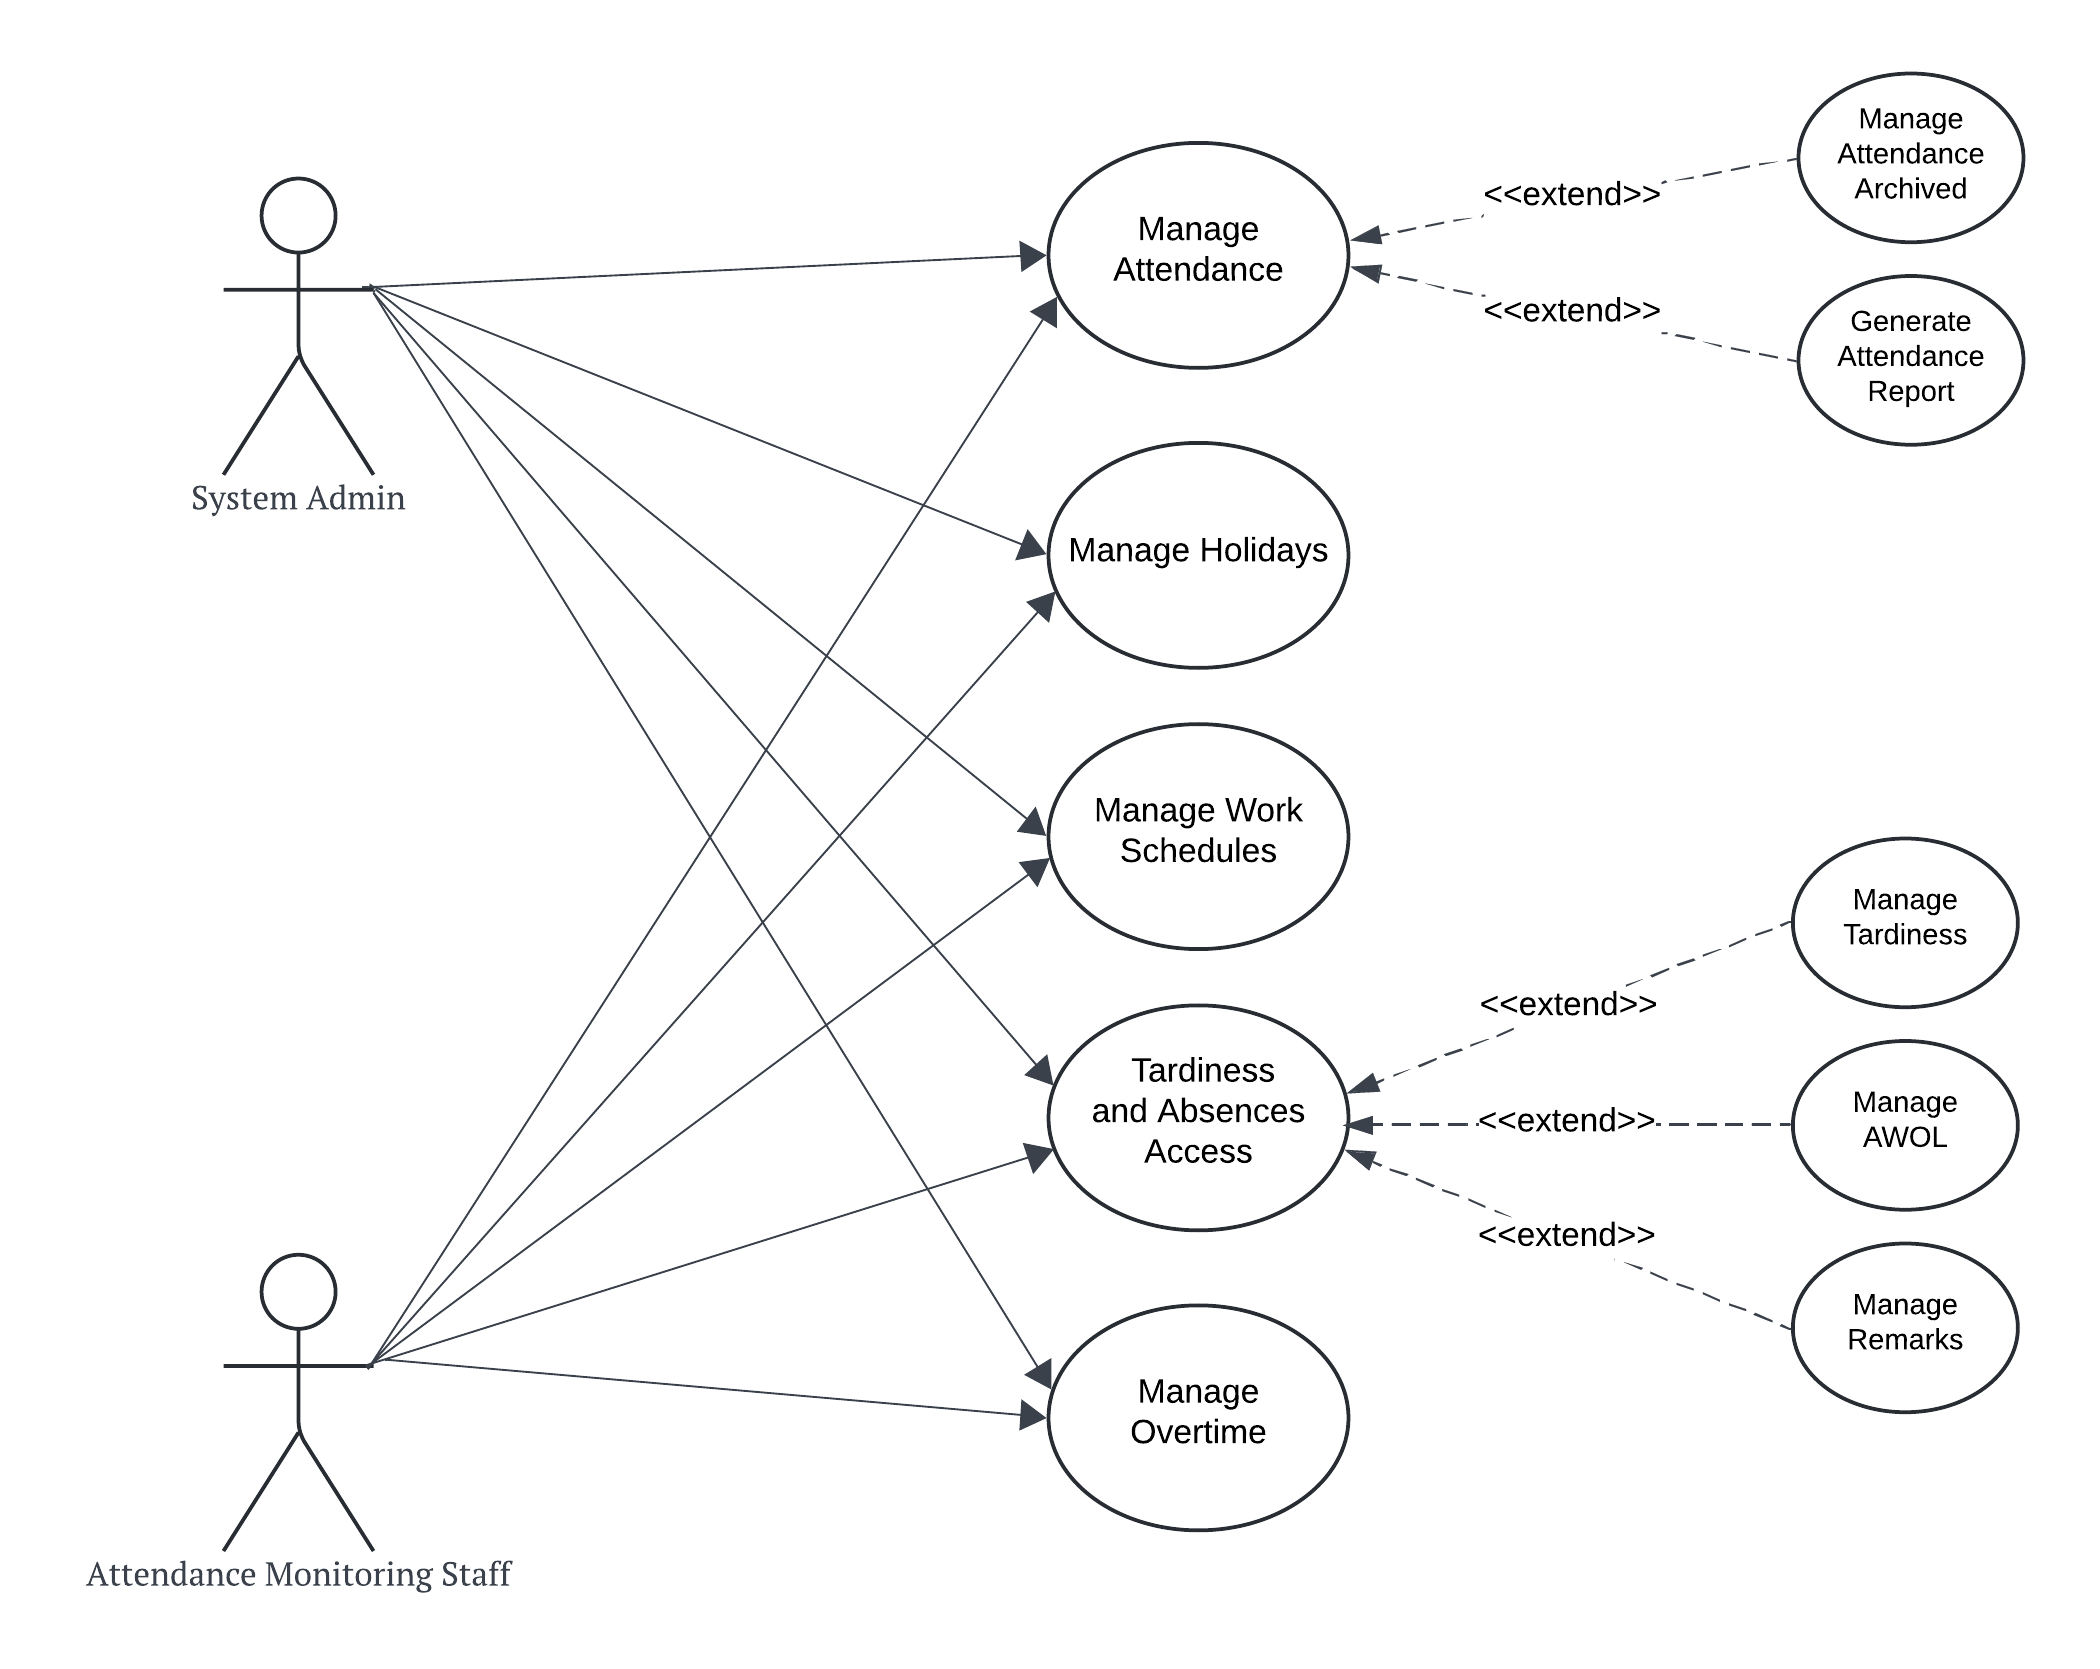
\includegraphics[width=0.9\linewidth]{figures/images/diagrams/usecase/use-case-time-1.png}
        \caption{HRIS TIMESYS Module: System Admin and Attendance Monitoring Staff.}
        \label{fig:use-case-time-1}
    \end{figure}

    The figure \ref{fig:use-case-time-1} demonstrates the use case diagram for the HRIS TIMESYS Module. The diagram shows the use cases for the System Admin and Attendance Monitoring Staff. Both of the actors have full managing access to all use cases found within the TIMESYS module. This comprehensive access enables the System Admin and Attendance Monitoring Staff to oversee and manage all aspects of the TIMESYS module, ensuring efficient and effective attendance monitoring and management.

    \begin{figure}[H]
        \centering
        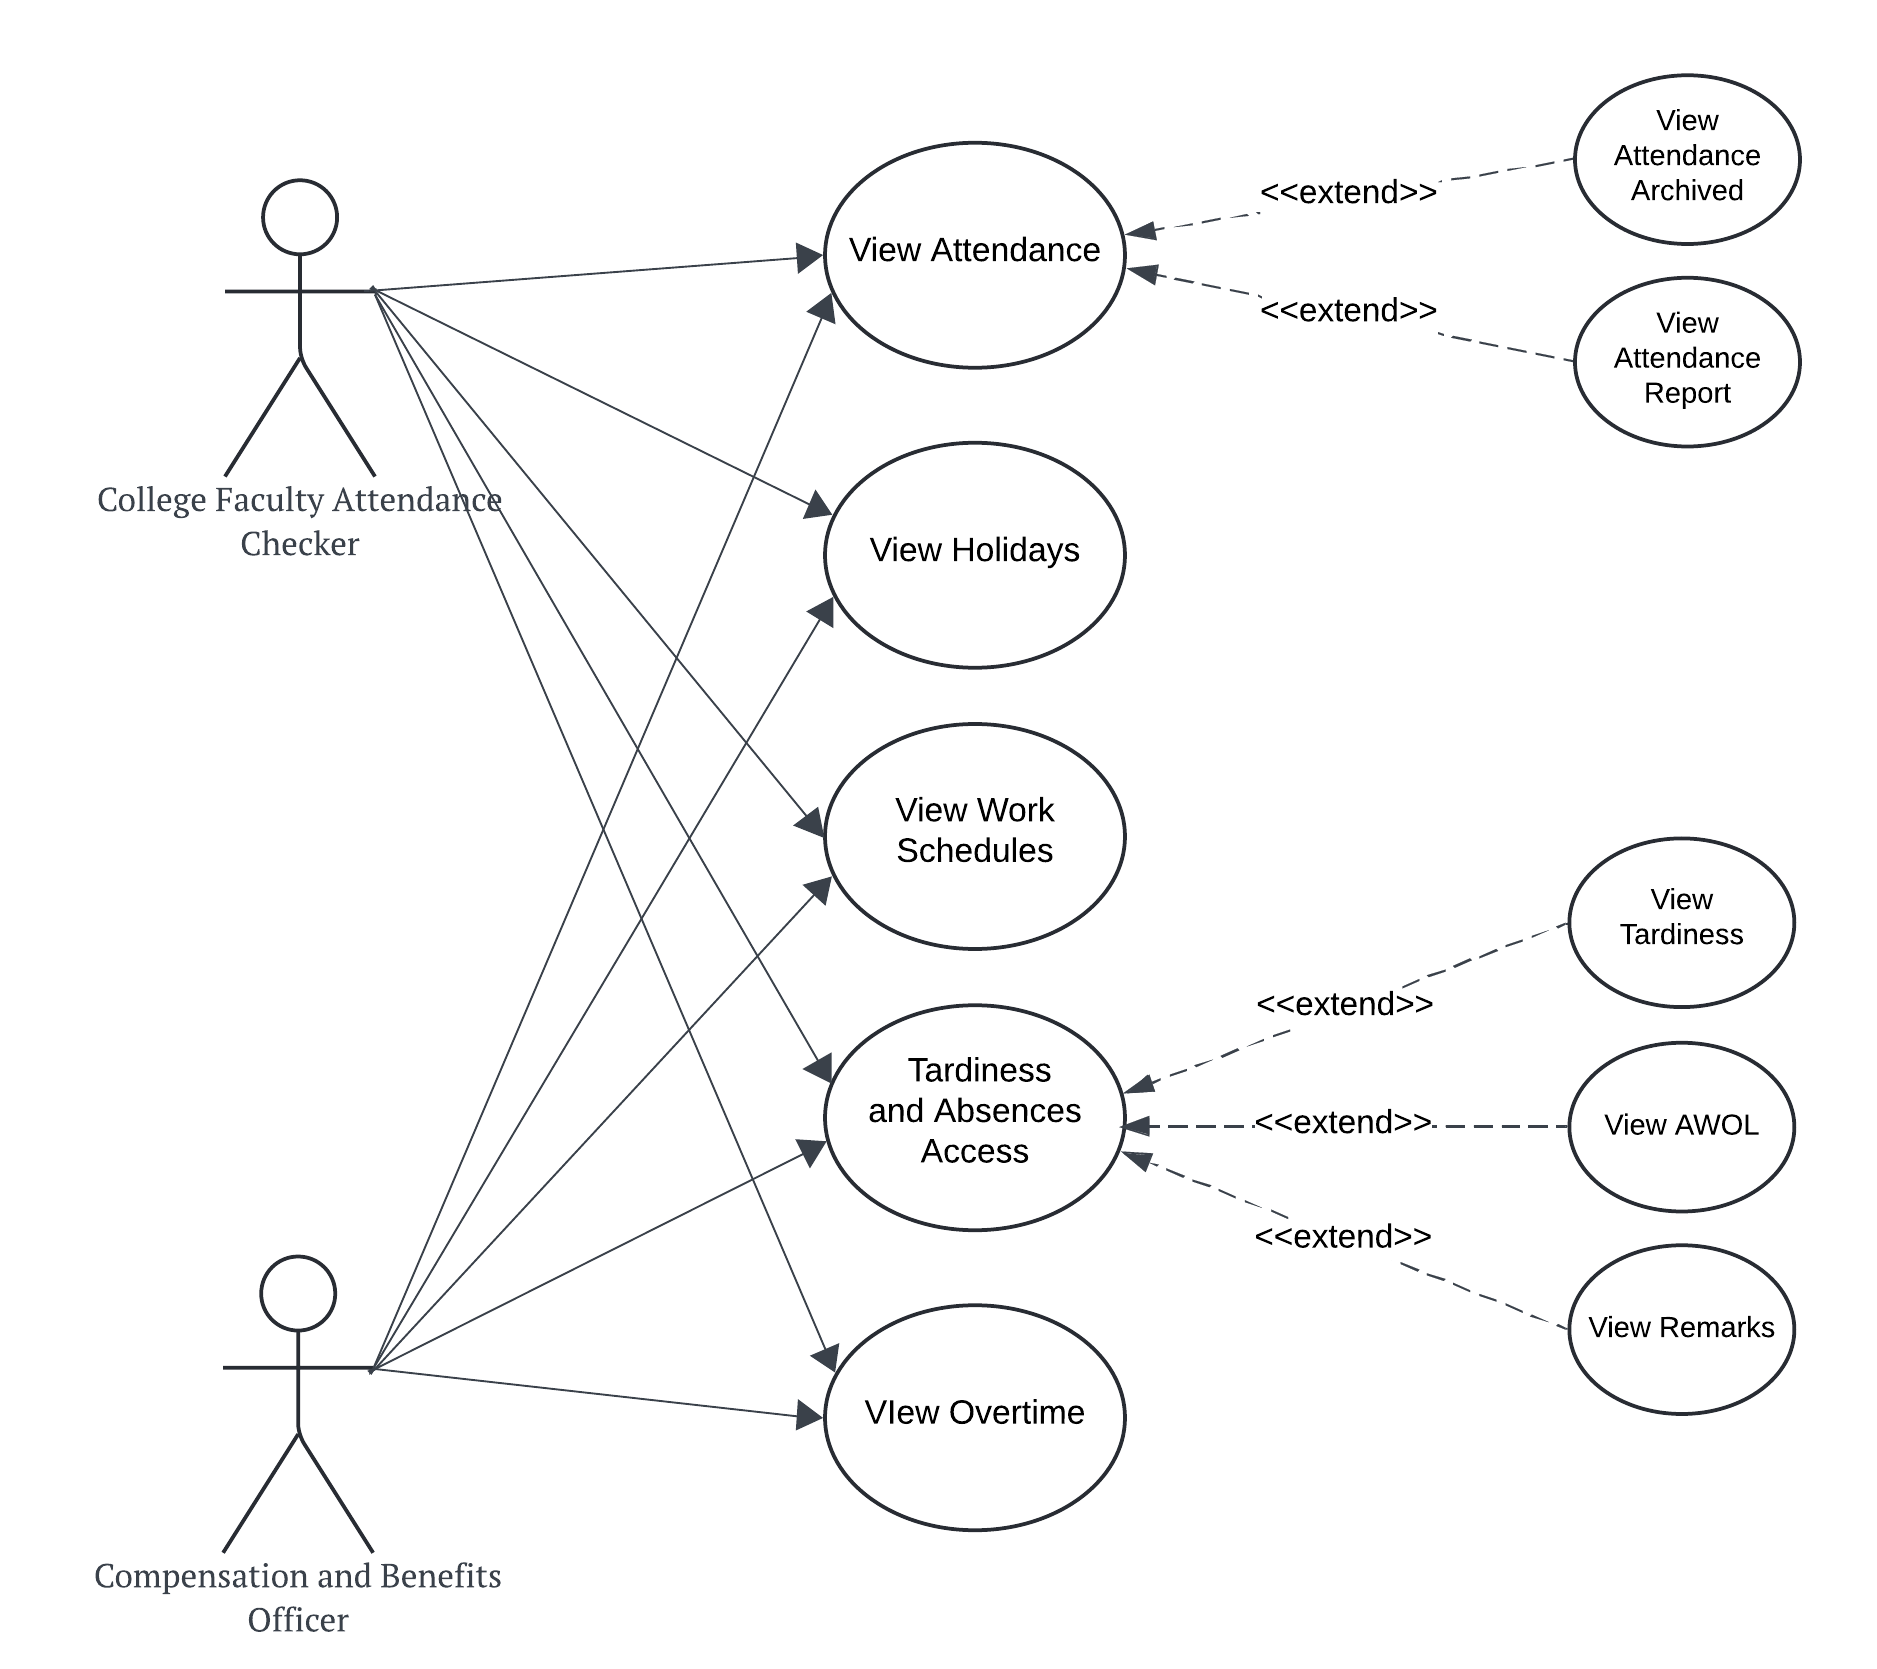
\includegraphics[width=0.9\linewidth]{figures/images/diagrams/usecase/use-case-time-2.png}
        \caption{HRIS TIMESYS Module: College Faculty Attendance Checker and Compensation and Benefits Officer.}
        \label{fig:use-case-time-2}
    \end{figure}

    The figure \ref{fig:use-case-time-2} depicts the use case diagram for the HRIS TIMESYS Module. The diagram illustrates the use cases for the College Faculty Attendance Checker and Compensation and Benefits Officer. Both actors share the same access which is limited to view-only access to all use cases found within the TIMESYS module. 


    In this section, it presents the use case diagrams for the HRIS FACSYS Module. The module involves five primary actors: System Admin, Attendance Monitoring Staff, College Faculty Attendance Checker, Compensation and Benefits Officer, and Student Assistant Attendance Checker. Each actor has specific access to various use cases within the FACSYS module, enabling them to perform functions related to faculty attendance monitoring and management. The FACSYS module consists of three primary use cases: Managing Faculty Attendance, which extends to the generation of faculty attendance reports; Managing Faculty Schedule, which includes handling pending faculty schedules; and Managing Required Class Hours. This structure ensures comprehensive coverage of all faculty attendance-related aspects of employee management.

    \begin{figure}[H]
        \centering
        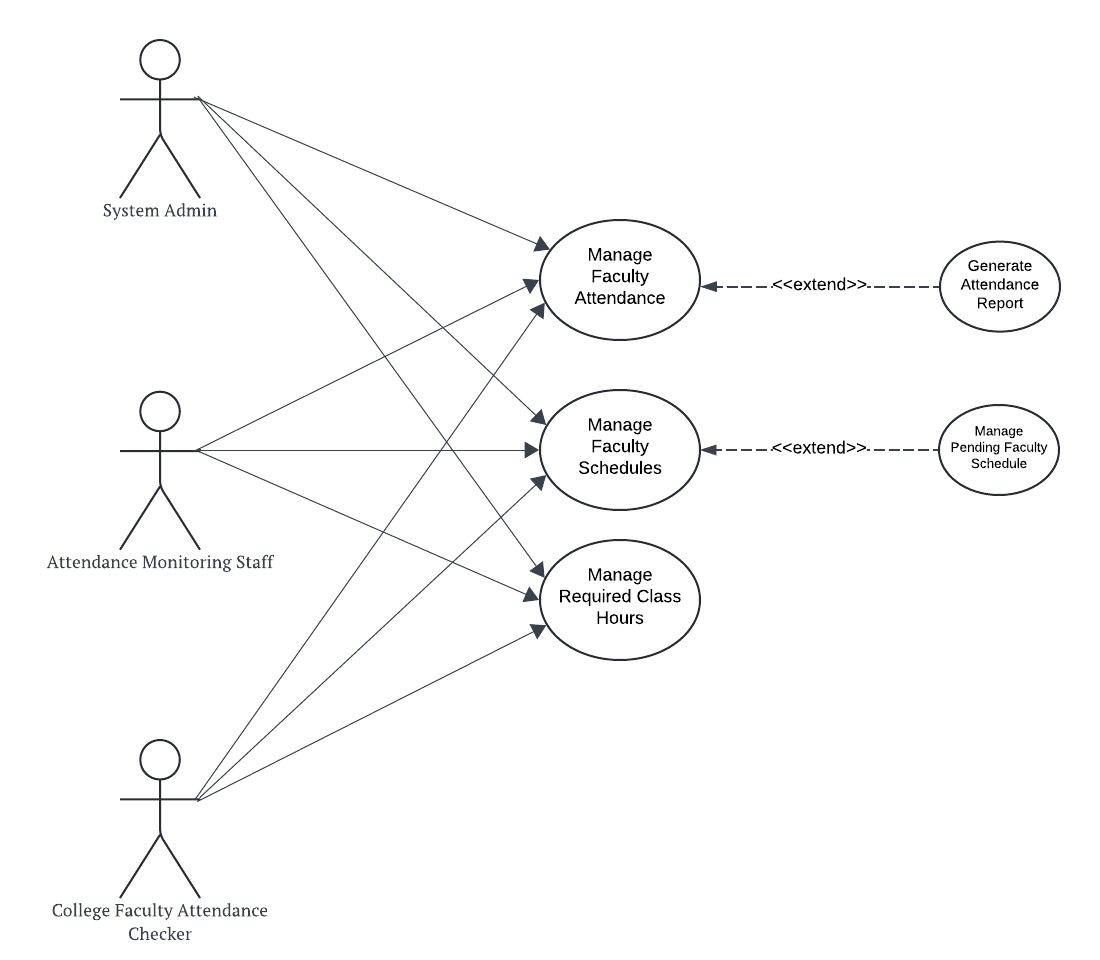
\includegraphics[width=0.9\linewidth]{figures/images/diagrams/usecase/use-case-fac-1.png}
        \caption{HRIS FACSYS Module: System Admin, Attendance Monitoring Staff, and College Faculty Attendance Checker.}
        \label{fig:use-case-fac-1}
    \end{figure}

    The figure \ref{fig:use-case-fac-1} illustrates the use case diagram of the System Admin, Attendance Monitoring Staff, and College Faculty Attendance Checker within the HRIS FACSYS Module. These three actors share the same full managing access to all use cases found within the FACSYS module. This comprehensive access enables the System Admin, Attendance Monitoring Staff, and College Faculty Attendance Checker to oversee and manage all aspects of the FACSYS module, ensuring efficient and effective faculty attendance monitoring and management.

    \begin{figure}[H]
        \centering
        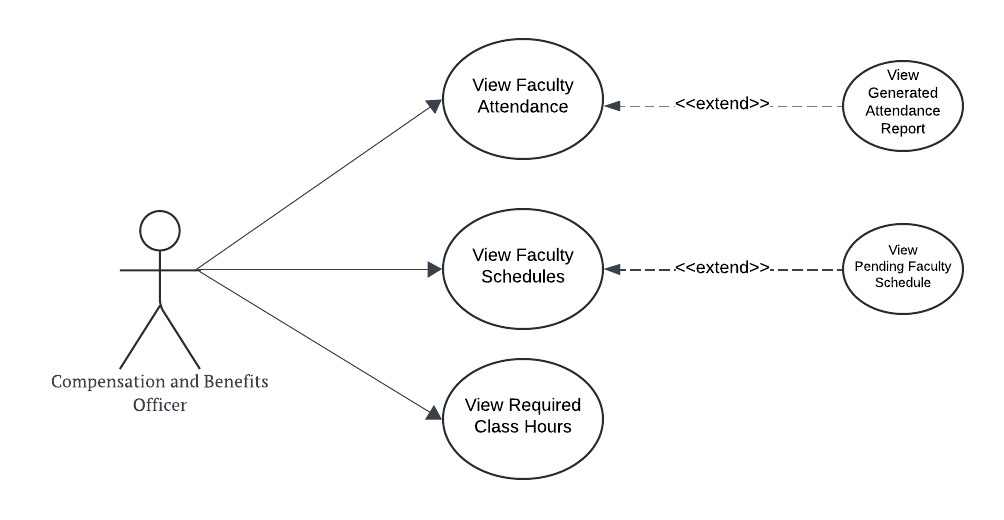
\includegraphics[width=0.9\linewidth]{figures/images/diagrams/usecase/use-case-fac-2.png}
        \caption{HRIS FACSYS Module: Compensation and Benefits Officer.}
        \label{fig:use-case-fac-2}
    \end{figure}

    The figure \ref{fig:use-case-fac-2} shows the use case diagram for the Compensation and Benefits Officer. The actor has limited view access to all of the use cases found within the FACSYS module. This includes Viewing Faculty Attendance, which extends to viewing of generated faculty attendance report; Viewing Faculty Schedule, which includes viewing of pending faculty schedules; and Viewing Required Class Hours. This structure ensures that the Compensation and Benefits Officer has the necessary access to view faculty attendance and schedule information, facilitating efficient monitoring and management of faculty attendance.

    \begin{figure}[H]
        \centering
        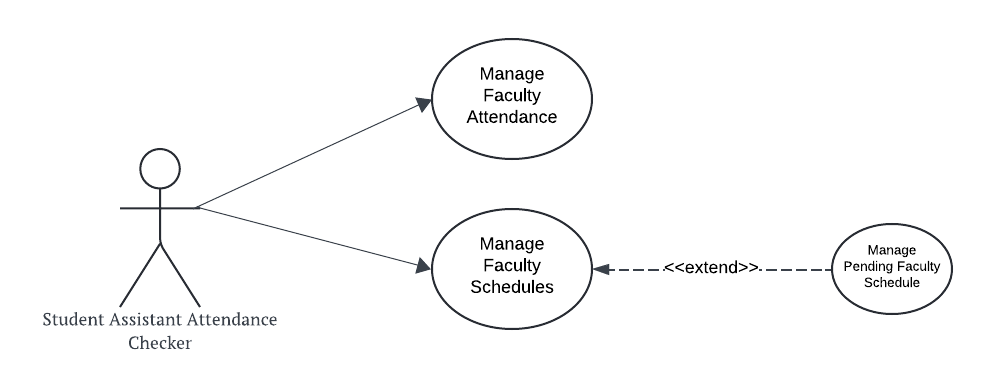
\includegraphics[width=0.9\linewidth]{figures/images/diagrams/usecase/use-case-fac-3.png}
        \caption{HRIS FACSYS Module: Student Asssitant Attendance Checker.}
        \label{fig:use-case-fac-3}
    \end{figure}

    The figure \ref{fig:use-case-fac-3} illustrates the use case diagram for the Student Assistant Attendance Checker. The actor has limited manage access to the use cases found within the FACSYS module. The Student Assistant Attendance Checker has the privilege to manage faculty attendance but wasn't able to generate faculty attendance report, and manage faculty schedule as well as managing the pending faculty schedules. This structure ensures that the Student Assistant Attendance Checker has the necessary access to manage faculty attendance, facilitating efficient monitoring and management of faculty attendance. 
    

    This section presents the use case diagrams for the HRIS LEAVESYS Module. The module involves four primary actors: System Admin, Attendance Monitoring Staff, College Faculty Attendance Checker, and Compensation and Benefits Officer. Each actor has specific access to various use cases within the LEAVESYS module, enabling them to perform functions related to employee leave management and processing. The LEAVESYS module consists of two primary use cases: Managing Leave Applications and Managing Leave Credits. The Managing Leave Applications use case extends to the management of leave reasons, while both Managing Leave Applications and Managing Leave Credits extend to the generation of leave application with Credits Report. This structure allows for comprehensive leave management, encompassing application processing, credit tracking, and reporting functionalities.

    \begin{figure}[H]
        \centering
        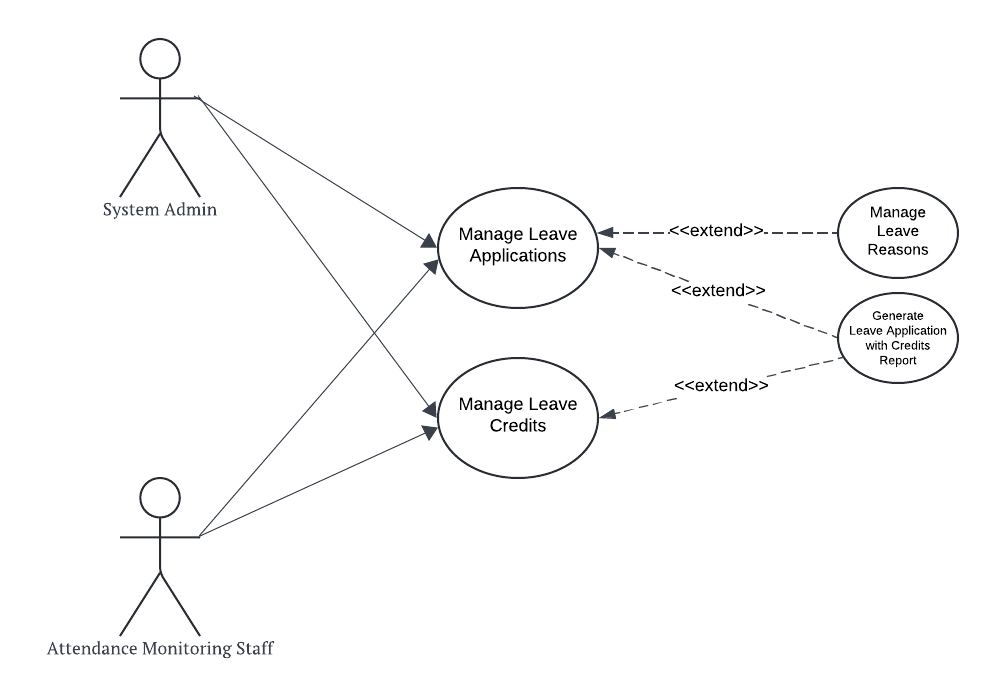
\includegraphics[width=0.9\linewidth]{figures/images/diagrams/usecase/use-case-leave-1.png}
        \caption{HRIS LEAVESYS Module: System Admin and Attendance Monitoring Staff.}
        \label{fig:use-case-leave-1}
    \end{figure}

    Figure \ref{fig:use-case-leave-1} illustrates the use case diagram for the System Admin and Attendance Monitoring Staff within the HRIS LEAVESYS Module. Both actors share full management access to all use cases within the LEAVESYS module. This includes Managing Leave Applications, which extends to managing leave reasons; and Managing Leave Credits. Both of the actors are able to Generate Leave Application with Credits Report. This comprehensive access enables the System Admin and Attendance Monitoring Staff to oversee and manage all aspects of the LEAVESYS module, ensuring efficient and effective leave management and processing.

    \begin{figure}[H]
        \centering
        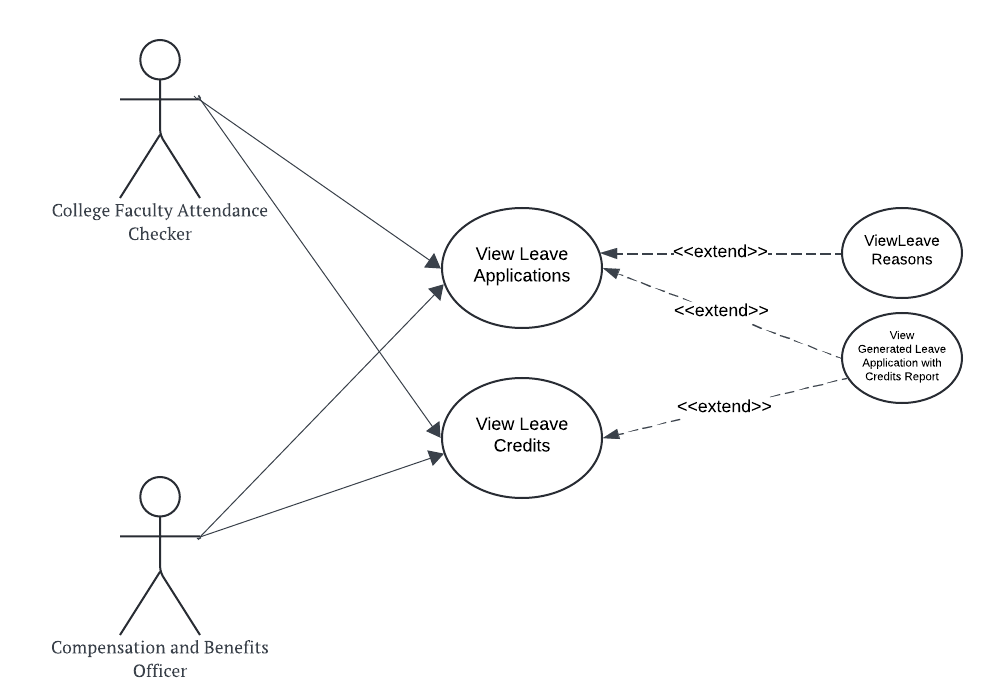
\includegraphics[width=0.9\linewidth]{figures/images/diagrams/usecase/use-case-leave-2.png}
        \caption{HRIS LEAVESYS Module: College Faculty Attendance Checker and Compensation and Benefits Officer.}
        \label{fig:use-case-leave-2}
    \end{figure}

    The figure \ref{fig:use-case-leave-2} depicts the use case diagram for the College Faculty Attendance Checker and Compensation and Benefits Officer within the HRIS LEAVESYS Module. Both actors share the same access which is limited to view-only access to all use cases found within the LEAVESYS module. This includes Viewing Leave Applications, which extends to viewing leave reasons; and Viewing Leave Credits. Both of the actors are only limited to viewing the Generated Leave Application with Credits Report. This structure ensures that the College Faculty Attendance Checker and Compensation and Benefits Officer have the necessary access to view leave applications, credits, and reports, facilitating efficient leave management and processing.


    \subsection{Entity Relational Diagram}
    
    The Entity Relational Diagram (ERD) will be used to visually represent the database structure that defines the relationships between different entities in the system and how they are related to one another through cardinalities and relationships. In the case of the HRIS application, MIS has provided ready access to the database scheme in preparation for the migration process. This ERD represents the various entities such as employees, departments, positions, and their relationships with each other. 
    
    Creating an ERD will allow the developers to design a database schema that accurately represents the data requirements of the HRIS system. This diagram is not only crucial for ensuring data integrity, normalization, and efficient data retrieval, but will also standardize and comply with the DBA requirements of the MIS for merge request and reviewing processes.

    \begin{figure}[H]
        \centering
        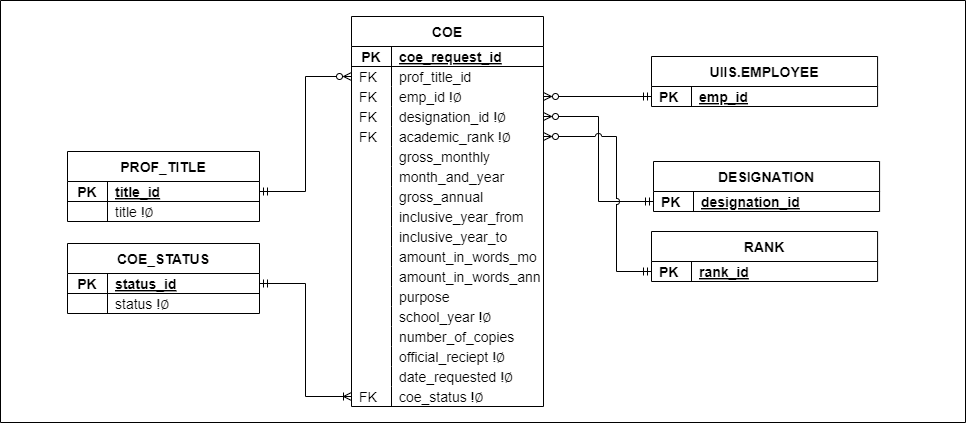
\includegraphics[width=1\linewidth]{figures/images/diagrams/erd/erd-core-coe.png}
        \caption{HRIS Core: Certificate of Employment ERD Model.}
        \label{fig:erd-core-coe} 
    \end{figure}

    This segment of the ERD model illustrates the Certificate of Employment (COE) module within the Human Resource Information System. The system is designed to efficiently manage and generate Certificates of Employment, incorporating various relevant factors for comprehensive employee documentation. Central to this module is the \texttt{hr.coe} entity, which is intricately connected to several other key entities. It links to \texttt{uiis.employee} for essential employee data, ensuring accurate personal information. The system also incorporates \texttt{hr.prof\_title} for the employee's professional designation, \texttt{hr.coe\_status} to track the current status of each certificate, \texttt{hr.office\_unit} to associate the employee with their specific department, \texttt{hr.designation} to capture the official job title, \texttt{hr.rank} to include information about the employee's hierarchical position, and \texttt{hr.employee\_status} to indicate their current employment arrangement. This structure enables the system to generate comprehensive and accurate Certificates of Employment, pulling relevant information from interconnected entities.

    \begin{figure}[H]
        \centering
        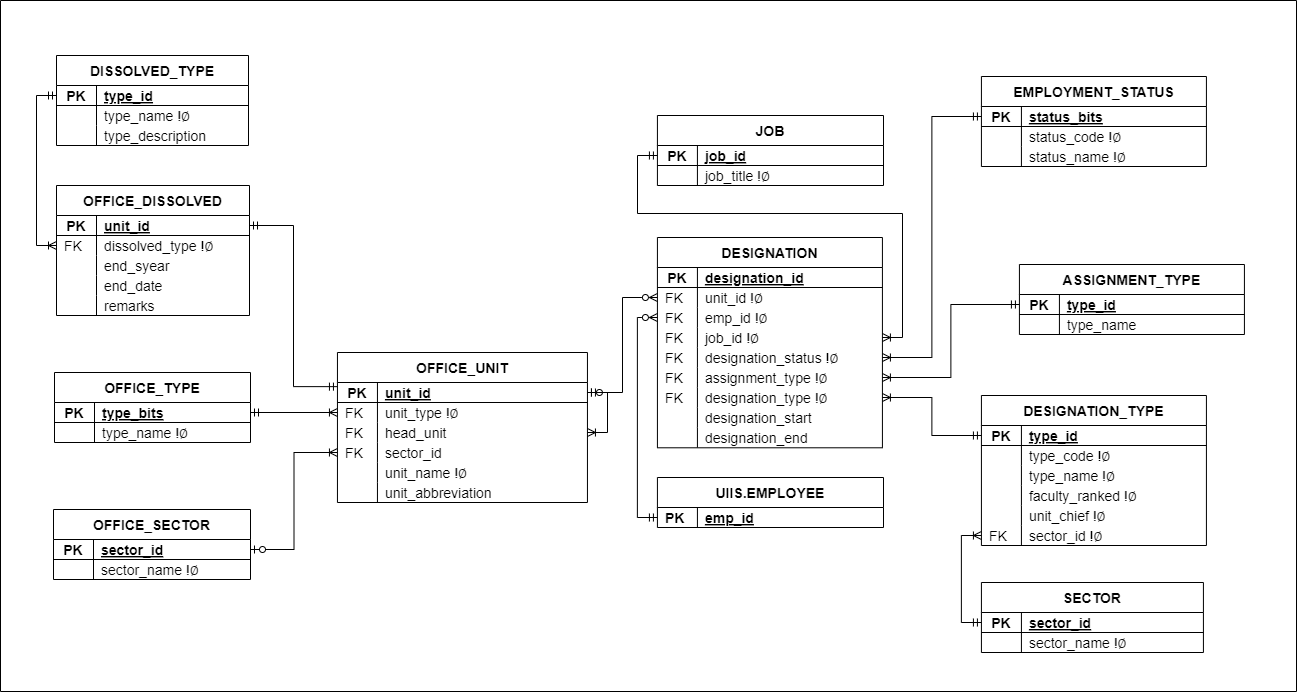
\includegraphics[width=1\linewidth]{figures/images/diagrams/erd/erd-core-office.png}
        \caption{HRIS Core: Designation ERD Model.}
        \label{fig:erd-core-office}
    \end{figure}

    The illutstration shows the ERD model for the designation module which is designed to manage the complex organizational structure and employee positions within the institution. The central \texttt{hr.designation} entity is linked to several other entities, providing a comprehensive view of each employee's position and organizational context. It connects to \texttt{uiis.employee} for individual employee data, \texttt{hr.office\_unit} for departmental information, and \texttt{hr.job} for specific job titles. The system incorporates \texttt{hr.employment\_status} to track the nature of employment (e.g., full-time, part-time), \texttt{hr.assignment\_type} for the kind of role assignment, and \texttt{hr.designation\_type} for categorizing positions. The \texttt{hr.designation\_type} entity further links to \texttt{hr.sector}, allowing for broader organizational grouping. The \texttt{hr.office\_unit} entity is part of a larger organizational structure, connecting to \texttt{hr.office\_sector} and \texttt{hr.office\_type} for detailed unit categorization. It also links to \texttt{hr.office\_dissolved} (which is also connects to \texttt{hr.dissolved\_type}), enabling the system to track historical changes in the organizational structure.

    \begin{figure}[H]
        \centering
        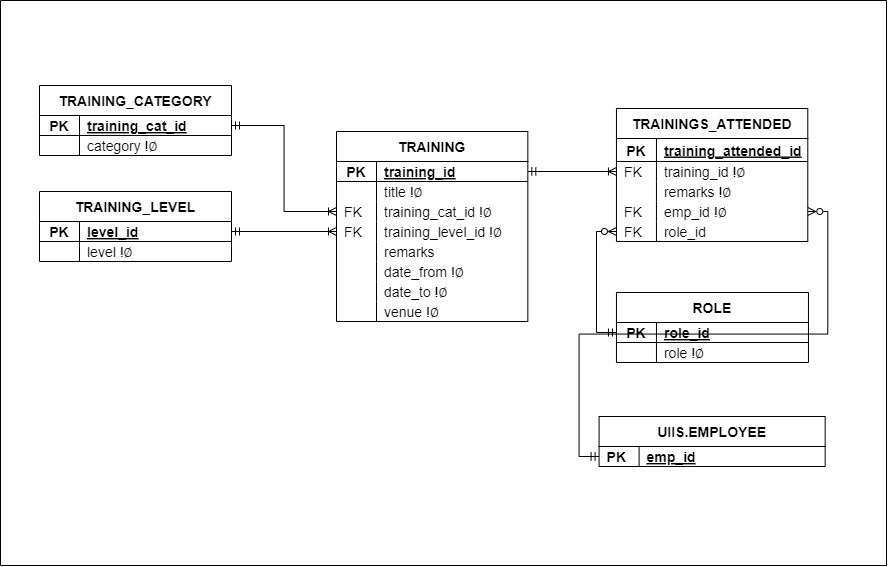
\includegraphics[width=1\linewidth]{figures/images/diagrams/erd/erd-core-trainings.png}
        \caption{HRIS Core: Trainings ERD Model.}
        \label{fig:erd-core-trainings}
    \end{figure}

    This part of the ERD model illustrates the Training module within the Human Resource Information System. The system is designed to comprehensively track and manage employee training activities. The central entity is \texttt{hr.training}, which captures essential details such as training title, date range, venue, and remarks. It's connected to \texttt{hr.training\_category} and \texttt{hr.training\_level}, allowing for classification of training types and levels of complexity or importance. The \texttt{hr.training\_attended} entity serves as a connection between individual employees \texttt{uiis.employee} and specific training sessions, also incorporating the \texttt{hr.role} of the employee in each training. This structure enables detailed recording of each employee's training history, including their role in each session.

    \begin{figure}[H]
        \centering
        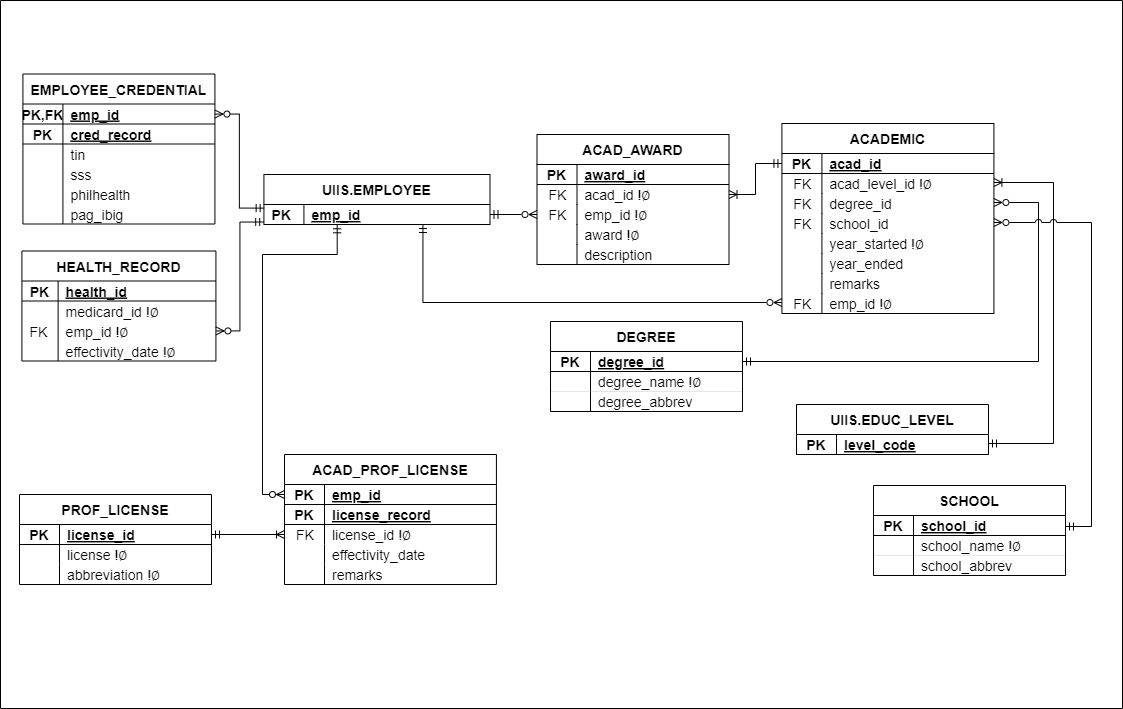
\includegraphics[width=1\linewidth]{figures/images/diagrams/erd/erd-core-emp-personal-info.png}
        \caption{HRIS Core: Employee Personal Information ERD Model.}
        \label{fig:erd-core-emp-personal-info}
    \end{figure}

    This segment of the Human Resource Information System is designed to manage comprehensive personal and professional information for each employee. The system revolves around the \texttt{uiis.employee} entity, which serves as the central point connecting various aspects of an employee's profile. The \texttt{hr.employee\_credential} entity stores essential identification and access information, directly linked to the employee record. Health-related information is captured in the \texttt{hr.health\_record} entity, ensuring that important medical id is securely associated with each employee. The \texttt{hr.academic} entity tracks educational background, connecting not only to the employee but also to \texttt{hr.school}, \texttt{uiis.educ\_level}, and \texttt{hr.degree} entities, allowing for a detailed educational history. 
            
    Academic achievements are recorded in the \texttt{hr.acad\_awards} entity, linked to both the employee and their academic records. Professional qualifications are managed through the \texttt{hr.acad\_prof\_license} entity, which connects employees to their professional licenses. This structure enables a holistic view of each employee's personal, educational, and professional qualifications, supporting various HR functions such as career development, compliance, and employee wellness initiatives.

    \begin{figure}[H]
        \centering
        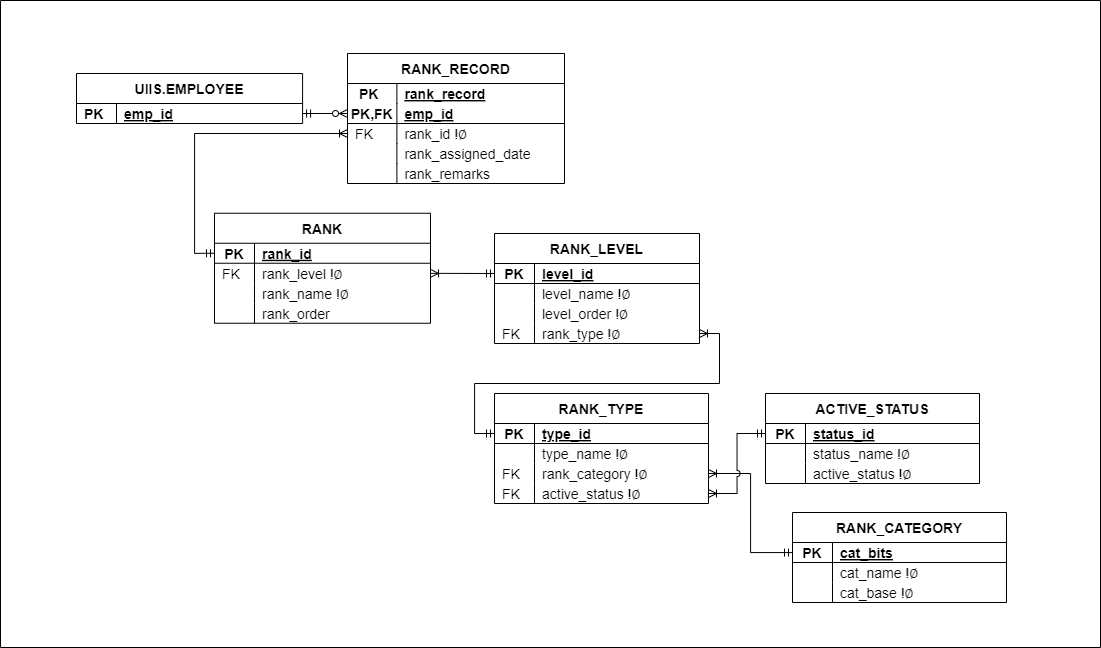
\includegraphics[width=1\linewidth]{figures/images/diagrams/erd/erd-core-rank.png}
        \caption{HRIS Core: Employee Rank ERD Model.}
        \label{fig:erd-core-rank}
    \end{figure}

    The Rank module in this HRIS is designed to manage the hierarchical structure of employee positions within the organization. The central \texttt{hr.rank\_record} entity is directly linked to \texttt{uiis.employee}, associating each employee with their current rank. This entity also connects to the \texttt{hr.rank} entity, which provides details about specific ranks. The \texttt{rank} entity is further linked to \texttt{hr.rank\_level}, allowing for a tiered structure of ranks. \texttt{hr.rank\_level}, then, is associated with \texttt{hr.rank\_type}, which categorizes different types of ranks. The \texttt{hr.rank\_type} entity is connected to both \texttt{hr.rank\_category} and \texttt{hr.active\_status}, enabling the system to classify ranks into broader categories and track their current status. 
            
    This hierarchical structure allows for detailed management of employee rankings, supports career progression tracking, and can facilitate reporting on organizational structure and employee distribution across different rank levels and categories.
    
    \begin{figure}[H]
        \centering
        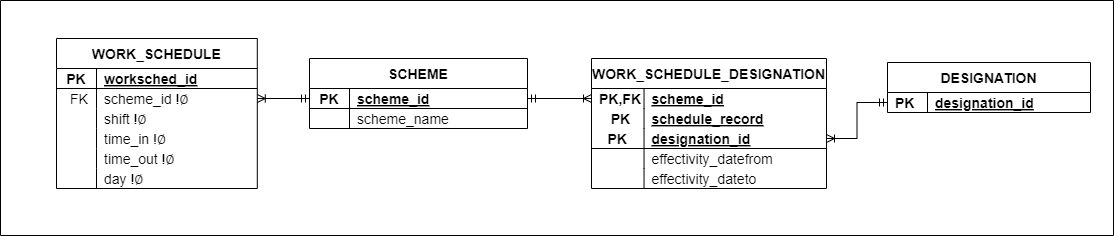
\includegraphics[width=1\linewidth]{figures/images/diagrams/erd/erd-timesys-work-schedule-scheme-and-assignment.png}
        \caption{HRIS TIMESYS: Work Schedule and Assignment ERD Model.}
        \label{fig:erd-timesys-work-schedule-scheme-and-assignment}
    \end{figure}

    The work schedule scheme and assignment module in the HRIS TIMESYS is designed to manage employee work schedules and assignments. The HR manages employee schedules by first defining schemes with assigned work schedules, shift, time-in/out, and day. The HR then assigns these scheme unto the employee under \texttt{hr.work\_schedule\_scheme\_designation}. This work schedule shall be used in reference for other tables within the schema.

    \begin{figure}[H]
        \centering
        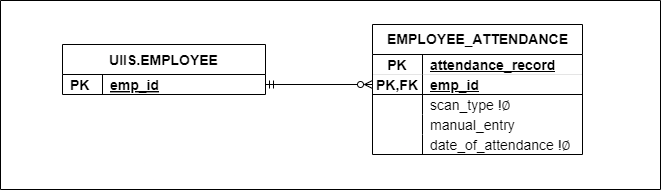
\includegraphics[width=1\linewidth]{figures/images/diagrams/erd/erd-timesys-employee-attendance.png}
        \caption{HRIS TIMESYS: Employee Attendance ERD Model.}
        \label{fig:erd-timesys-employee-attendance}
    \end{figure}

    One of the crucial components of the HRIS TIMESYS module is the employee attendance management system. The structure is designed to capture employee attendance data, including date, time, manual adjustment, and scan types as employees within the University is required to log in their attendance through RFID scanners. The \texttt{hr.employee\_attendance} entity will be the central point for recording not just for recording attendances but will also be used to compute for the employee's tardiness and overtime.

    \begin{figure}[H]
        \centering
        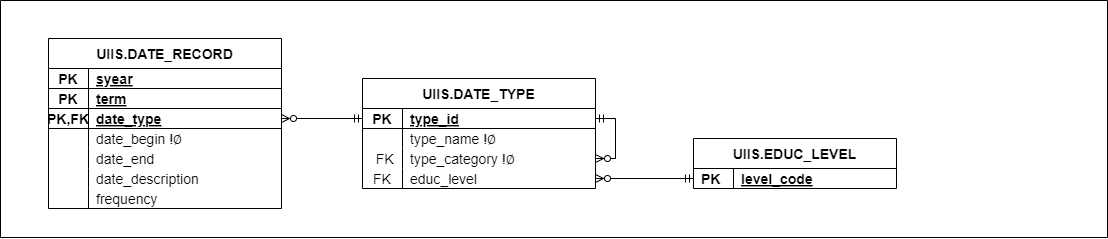
\includegraphics[width=1\linewidth]{figures/images/diagrams/erd/erd-timesys-holiday.png}
        \caption{HRIS TIMESYS: Holiday ERD Model.}
        \label{fig:erd-timesys-holiday}
    \end{figure}

    The holiday module in the HRIS TIMESYS is designed to manage non-working days that should not be counted as absences. The \texttt{hr.date\_record} entity captures detailed information about each holiday, including the date, name, and remarks. The primary purpose for utilizing a customized event management system for holidays is to ensure that employee leave records accurately reflect non-working days. 

    \begin{figure}[H]
        \centering
        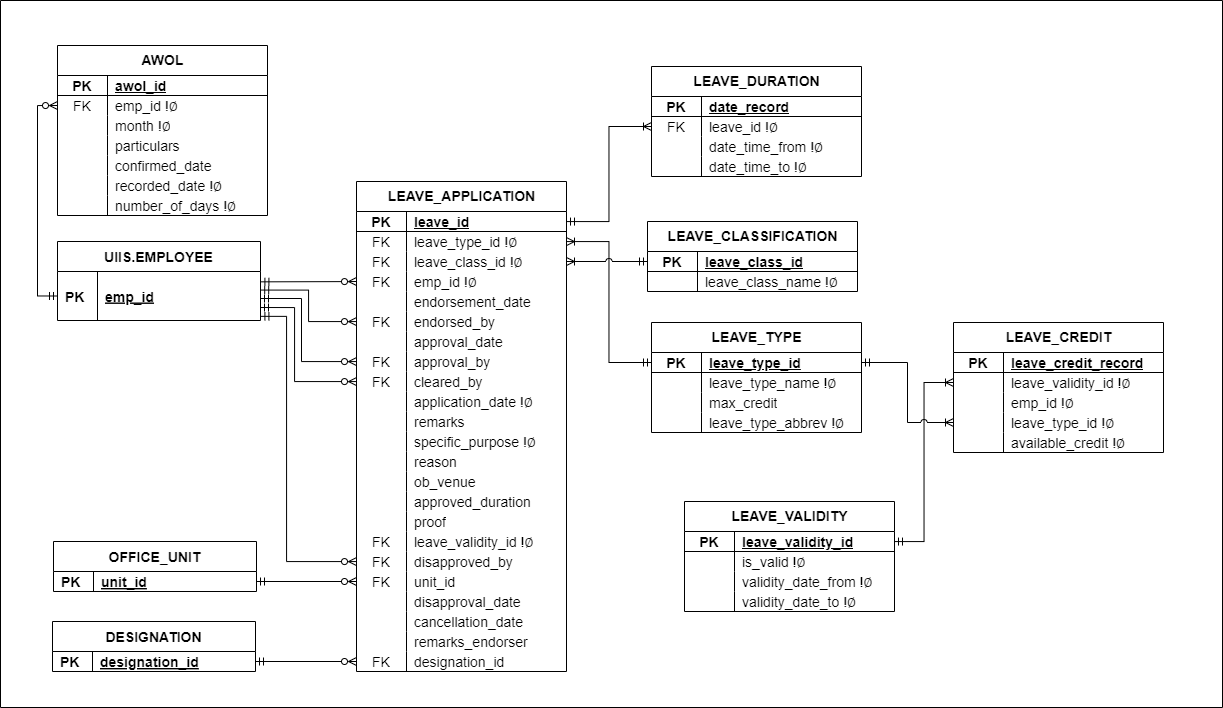
\includegraphics[width=1\linewidth]{figures/images/diagrams/erd/erd-leavesys-employee-leave.png}
        \caption{HRIS LEAVESYS ERD Model.}
        \label{fig:erd-leavesys-employee-leave}
    \end{figure}

    Among the key modules in the HRIS is a module for handling leave applications within the University. This includes handling leave from employees. The \texttt{hr.leave\_application} entity captures detailed information about each leave application, including the date, type, classification, reason, validity, and status. These leaves are then computed and deducted from the employee's leave credits and shall be used upon notifying the employees and for the HR's report.

    The system shall also capture Absent Without Leave (AWOL). The \texttt{hr.awol} entity captures recorded AWOLs, including the date, particulars, confirmed date, and number of days.

    \begin{figure}[H]
        \centering
        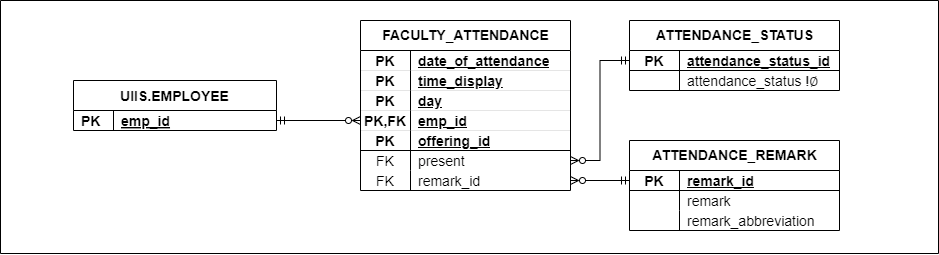
\includegraphics[width=1\linewidth]{figures/images/diagrams/erd/erd-facsys-faculty-attendance.png}
        \caption{HRIS FACSYS ERD Model.}
        \label{fig:erd-facsys-faculty-attendance}
    \end{figure}

    This segment of the ERD model illustrates the HRIS FACSYS module, which focuses on monitoring and recording faculty attendance. It centers around the \texttt{hr.faculty\_attendance} entity, which records detailed attendance information, including date, time, day, and associated course offerings for each employee. The system links to a separate \texttt{uiis.employee} entity, containing broader employee data. It incorporates two supporting entities: \texttt{hr.attendance\_status} for categorizing attendance and \texttt{hr.attendance\_remark} for additional notes. This structure allows for comprehensive tracking of faculty attendance, supporting multiple class offerings per employee and providing flexibility in recording attendance statuses and remarks. The design enables efficient record-keeping and could facilitate various attendance-related analyses and reports.

    \begin{figure}[H]
        \centering
        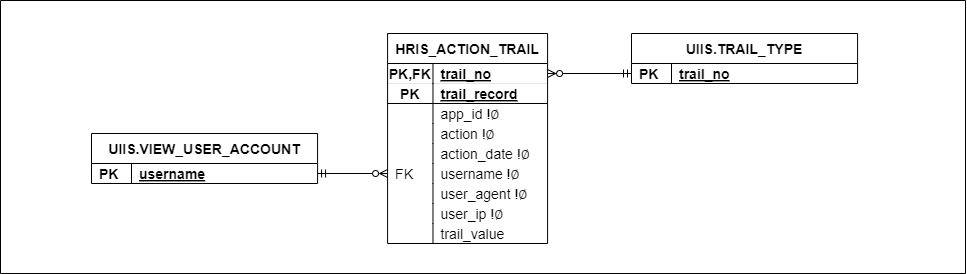
\includegraphics[width=1\linewidth]{figures/images/diagrams/erd/erd-trails.png}
        \caption{HRIS Trails ERD Model.}
        \label{fig:erd-trails}
    \end{figure}

    In order to ensure data integrity and accountability, the new HRIS shall incorporates trails that can tracks all system activities and changes. The trail captures the various entities involved in various modules The \texttt{HRIS\_TRAIL\_ACTION\_TRAIL} entity records the details of each system activity, including the action taken, the entity affected, and the user responsible. This allows for robust monitoring not just for HRMO but also for MIS and DBA to track system activities, changes, and user interactions. 

    This ERD has been reviewed and approved by the MIS DBA with a signed proof of acknowledgement in figure \ref{fig:proof-ack-aug-19} during consultation for this ERD. 
    
    \subsection{Gantt Chart}
    
    Gantt chart allows for a visual representation of the project schedule that outlines the tasks, milestones, and dependencies throughout the development time. In connection with the development of project management strategy through RAD, the HRIS application's use of a Gantt chart will help in planning and tracking the project's progress. It will break down the development process into specific tasks, assign responsibilities, and establish timelines for each phase of the project.
    
    With this, the development team can effectively manage resources, monitor progress, and ensure that the project stays on track to meet the specified deadlines.

    \begin{figure}[H]
        \centering
        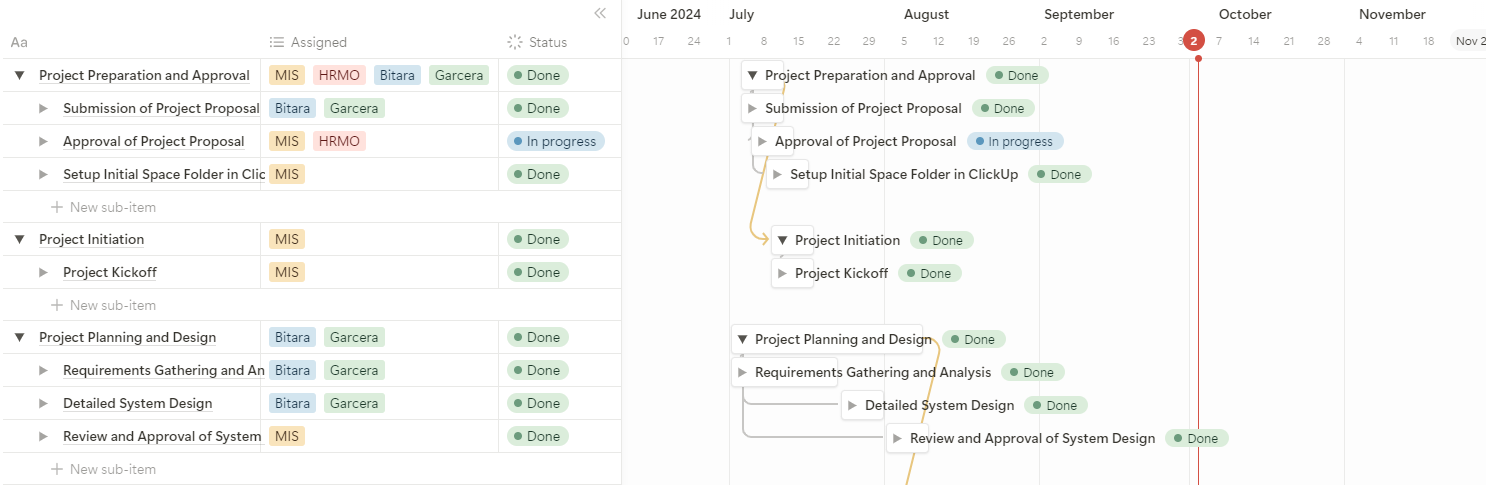
\includegraphics[width=1\linewidth]{figures/images/diagrams/gantt/gantt-chart-1.png}
        \caption{HRIS Gantt Chart Pre-planning Timeline.}
        \label{fig:gantt-chart-1}
    \end{figure}

    The gantt chart in figure \ref{fig:gantt-chart-1} illustrates the pre-planning timeline for the HRIS project. It outlines the key tasks and milestones that need to be completed before the development phase begins. This includes submission and approval of the project proposal, project management setup, to requirements gathering and system design. The timeline provides a clear overview of the project's initial stages and sets the foundation for the subsequent development phases.

    \begin{figure}[H]
        \centering
        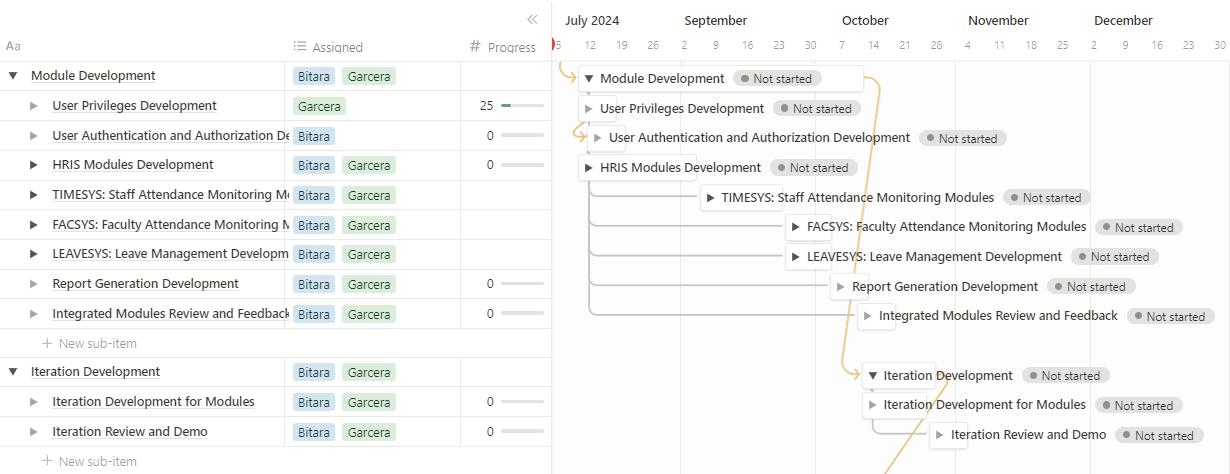
\includegraphics[width=1\linewidth]{figures/images/diagrams/gantt/gantt-chart-2.png}
        \caption{HRIS Gantt Chart Modules Development Timeline.}
        \label{fig:gantt-chart-2}
    \end{figure}

    In the figure \ref{fig:gantt-chart-2}, the gantt chart outlines the timeline for the modules development phase of the project. It breaks down the development process into specific tasks and assigns responsibilities to the development team. The timeline includes tasks from the user authentication to HR core modules, to TIMESYS, LEAVESYS, and FACSYS. During the development phase of the project, the developers shall also make iterations and adjustments based on user feedback and testing results.

    \begin{figure}[H]
        \centering
        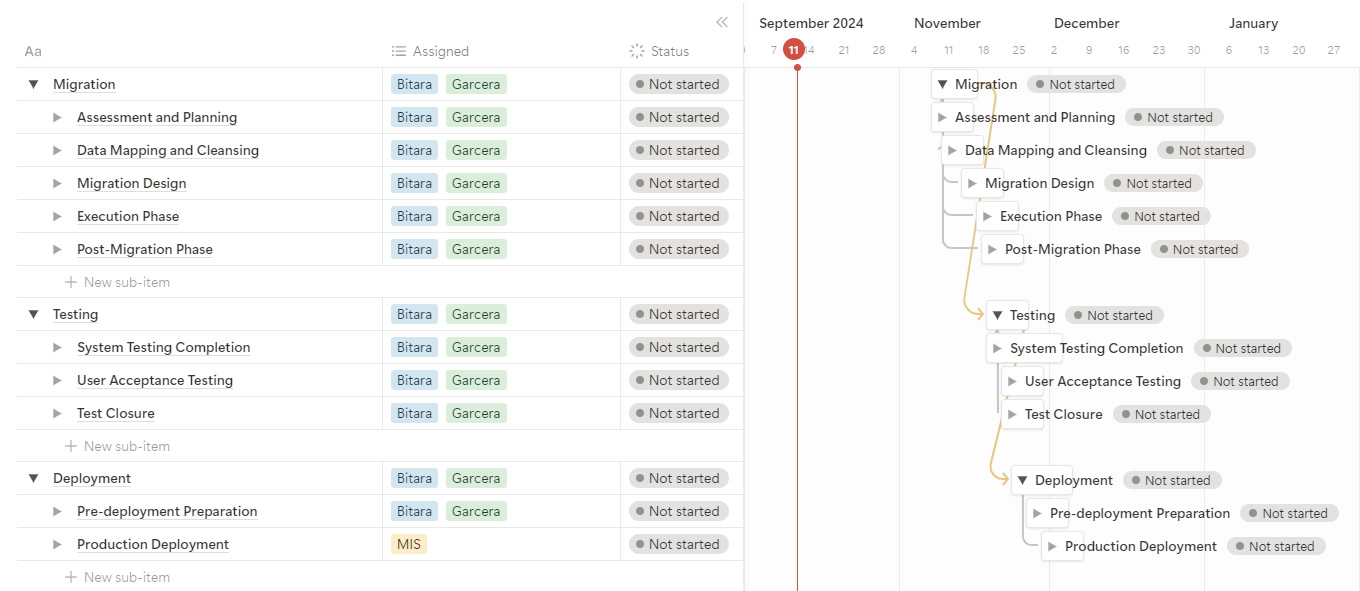
\includegraphics[width=1\linewidth]{figures/images/diagrams/gantt/gantt-chart-3.png}
        \caption{HRIS Gantt Migration to Deployment Timeline.}
        \label{fig:gantt-chart-3}
    \end{figure}

    In the figure \ref{fig:gantt-chart-3}, the gantt chart outlines the timeline for the migration phase of the project. Wherein, it will require other entities such as the HR, ISS, DBA, and MIS to work together to ensure a smooth transition of data from the existing HRIS system to the new HRIS application. The timeline includes migration plan, testing phase, and deployment phase.

    \begin{figure}[H]
        \centering
        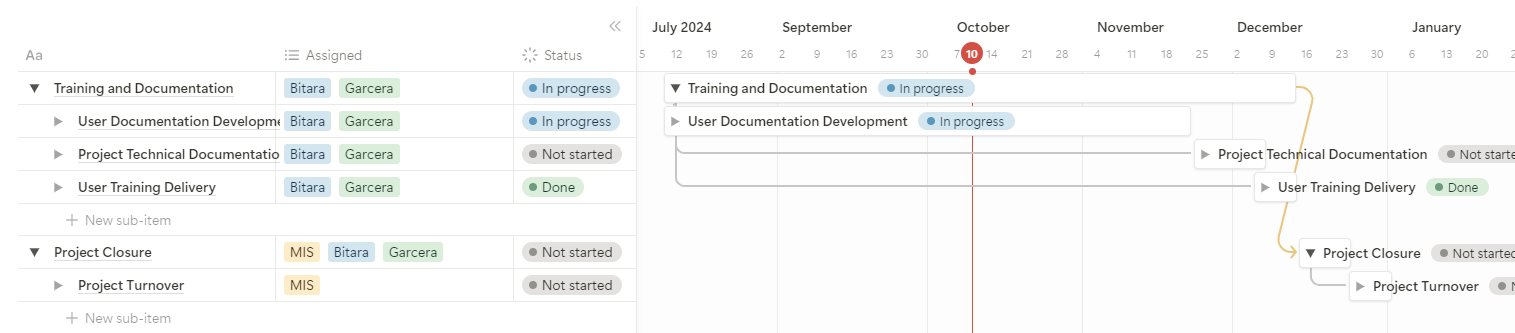
\includegraphics[width=1\linewidth]{figures/images/diagrams/gantt/gantt-chart-4.png}
        \caption{HRIS Gantt Post Development Timeline.}
        \label{fig:gantt-chart-4}
    \end{figure}

    After the deployment phase, the gantt chart in figure \ref{fig:gantt-chart-4} outlines the timeline for the post-development phase of the project. This includes creating trainings and documentations for the HRIS application, providing support, and monitoring the system's performance e.g., user manual, user trainings, and technical documentations. Once accomplished, the project will be handed over to MIS for further management and maintenance.

\section{Data Migration Plan}

    \subsection{Objectives}

    The data migration plan aims to ensure a smooth and efficient transition of data from the existing HRIS system to the new HRIS application. The key objectives of the data migration plan include:

    \begin{enumerate}
        \item Identify and extract relevant data from the existing HRIS system.
        \item Transform and map the data to align with the new HRIS database schema.
        \item Load the data into the new HRIS application while ensuring data integrity and accuracy.
        \item Validate the migrated data to ensure completeness and consistency.
        \item Minimize downtime and disruptions to the HR operation.
        \item Document the data migration process and outcomes for future reference.
    \end{enumerate}

    \subsection{Data Migration Strategy}

    The data migration strategy will involve the following key steps:
    
        \subsubsection{Assessment and Planning}
            This phase involves identifying the key stakeholders, analyzing the current HRIS that being utilized, gathering requirement for the new system. Having a proper assessment and planning are crucial in understanding the scope of the migration, identifying potential risks, and setting clear objectives. This phase ensures that all stakeholders are aligned and that the migration plan addresses all necessary aspects of the project. Also, effective planning will help mitigate risks and lays a solid foundation for the migration process.

        \subsubsection{Data Mapping and Cleansing}
            In this phase, it includes aligning the data fields from the legacy system to the new HRIS and correcting data quality issues. To ensure that all important data is correctly transferred to the new system, having an proper or accurate data mapping is needed. This phase also includes data cleansing as it is essential for maintaining data integrity and ensuring that the new system operates with accurate and reliable data. This step is critical for preventing data-related issues post-migration and ensuring a smooth transition.

        \subsubsection{Migration Design}
            The Migration design involves selecting migration tools  and deciding on the migration approach. Choosing the necessary and right tools and approach can significantly reduce the risk of errors and downtime. With a well-designed migration process ensures that data is transferred efficiently and securely. This step is important for optimizing the migration process and ensuring that it aligns with the project's goals and constraints
        
    \subsection{Execution Phase}
        \subsubsection{Pilot Migration}
            Conducting a pilot migration involves setting up a test environment and performing a trial run with a subset of data. A pilot migration helps identify potential issues and validate the migration process before the full migration. Also, with this step it will be helpful for minimizing risks and ensuring a smooth transition. It allows for adjustments to be made based on the findings from the pilot, thereby improving the overall migration strategy

        \subsubsection{Full Migration}
            In this full migration, it involves extracting, transforming, and loading the full dataset into the new system. Proper execution ensures that all data is accurately transferred and that the new system is ready for use. Validation and reconciliation are essential to confirm data integrity and completeness. This step is the core of the project and requires meticulous planning and execution to ensure success

    \subsection{Post-Migration Phase}
        Post-migration activities include system testing, data validation, user training, and providing support. These activities ensure that the new system operates correctly, that data integrity is maintained, and that users are comfortable with the new system. Ongoing support helps address any issues that arise after the migration. This step is crucial for ensuring the long-term success of the new system and for achieving user satisfaction
    
\section{System Testing Plan}

    The system testing phase aims to comprehensively evaluate the functionality, performance, and reliability of the application. To ensure a thorough assessment, we have established the following key objectives within the system testing plan:
    
    \begin{enumerate}
        \item Verify the functionality of all system features and modules.
        \item Ensure the system meets all specified requirements.
        \item Identify and document any bugs or issues.
        \item Validate the system's performance and response times.
        \item Test the user interface for usability and intuitiveness.
        \item Confirm data integrity and security measures.
        \item Assess the system's compatibility with different browsers and devices.
    \end{enumerate}

    \subsection{Participants}

    Throughout the testing phase, the participants will include the HR managers as well as the Information System Administrator, and the DBA Administrators.

    \subsection{Equipment and Hardware Requirements}

    The requirements for using the application is minimal due to its chosen deployed platform -- web. The application will only require any modern device that can access the internet through modern up-to-date browsers; specifically Google Chrome version 96 and above. 
    
    The testing phase will be conducted within University grounds as it will require the University's internal network for it to be accessed. 

\section{System Deployment Plan}

This section contains some of the high-level tasks and considerations that will be addressed during the deployment phase of the newly developed and migrated ADNU HRIS.

    \subsection{Deployment Planning}
        
        The deployment plan identifies the requirements and responsibilities of both the client and the development team in preparation for deployment. This includes accomplishing HR requirements -- HR core modules, TIMESYS, LEAVESYS, and FACSYS after reaching satisfaction within the testing plan.

    \subsection{Resources}
        \subsubsection{Facilities}

        The facilities required for testing and deployment to the new HRIS will be conducted within the HR office grounds equipped with modern computers as well a reliable and high-speed internet connection.

        \subsubsection{Hardware}

        The hardware required for running the application shall include:

        \begin{enumerate}
            \item Desktop Computers/Laptops
            \begin{enumerate}
                \item \textbf{Processor:} Minimum Intel Core i3 or AMD equivalent
                \item \textbf{RAM:} Minimum of 4GB (recommended 8GB or higher)
                \item \textbf{Storage:} Minimum of 128GB (recommended 256GB or higher)
            \end{enumerate}
            
            \item Backup and Recovery Hardware
            \begin{enumerate}
                \item \textbf{Backup Power supply:} This is to avoid downtime during any power outages to ensure uninterrupted workflow. Ensure that there is a Uninterruptible Power Supply (UPS) systems for critical hardware.
                
                \item \textbf{Electric Generators:} This is to for any extend outages that can occur within operations time. This ensures that the University can still cater and be operational despite the outages.
            \end{enumerate}
            
            \item Peripheral Devices
            \begin{enumerate}
                \item \textbf{DTR Scanner:} The HR module TIMESYS will utilize the DTR Scanner for employee attendance purposes.
                \item \textbf{RFID Scanner:} The RFID scanner will be utilized in support for the DTR within HR.
            \end{enumerate}
            
        \end{enumerate}

        \subsubsection{Support Software}

        As the project will utilize Oracle for the data migration, the supported software shall be to use Oracle 12c with instantclient12 installed and sqldeveloper for the database management solution. 

        Being a web-based application, the project requires to run on modern browsers with version 96 and above for Google Chrome. This ensures better up-to-date features and better security patches for each devices.

        \subsubsection{Support Documentation}

        The documentation required to support the application shall include:

        \begin{itemize}
            \item[] \textbf{User Manuals:} Detailed guides for end-users to navigate and utilize the HRIS effectively.
            \item[] \textbf{Technical Documentation:} In-depth documentation for developers detailing the system architecture, database schema, and configuration settings.
            \item[] \textbf{Training Materials:} Resources for training sessions, including slides, and user manuals.
            \item[] \textbf{FAQs and Troubleshooting Guides:} Common issues and their resolutions to assist users and support staff under user manual.
            \item[] \textbf{System Requirements:} Specifications for hardware, software, and network configurations needed to run the new HRIS.
        \end{itemize}

    \subsection{Deployment Strategies}
    
    The project will be deployed through a series of code review, database review, iteration, and installation of the developed app to the server after a series of testing and acceptance to the application. This process involves multiple personnel including the DB Administrator, Senior Application Developer, and Information System Administrator. 
    
    \subsection{Contingencies}
    
    Contingency plans are ensured to mitigate any potential issues that may arise during and after deployment, the following contingency plans will be put in place:

    \begin{itemize}
        \item[] \textbf{Rollback Plan:} A rollback strategy will be developed and practiced for each implementation to revert to the previous system in case of any critical failures during deployment. This includes utilizing version controls and maintaining a full backup of the old system.

        \item[] \textbf{Performance Monitoring:} Includes continuous monitor of system performance post-deployment through feedback and user reports from the HR for any performance degrade.
    \end{itemize}

    \subsection{Compatibility Strategies}
 
    To ensure smooth deployment and integration of the new ADNU HRIS, the following compatibility strategies will be implemented:
    
    \begin{itemize}
        \item[] \textbf{System Compatibility Testing:} Rigorous testing will be conducted to ensure the new HRIS is compatible with existing hardware, software, and network infrastructure at ADNU.
        
        \item[] \textbf{Browser Compatibility:} The web-based application will be tested across multiple browsers and versions to ensure consistent functionality and appearance.
        
        \item[] \textbf{Integration Testing:} Comprehensive testing will be performed to verify seamless integration with other existing systems and databases at ADNU.
        
        \item[] \textbf{Legacy System Compatibility:} Where necessary, interfaces or middleware will be developed to ensure compatibility with any legacy systems that need to interact with the new HRIS.
        
        \item[] \textbf{Scalability Testing:} The system will be tested to ensure it can handle increased load and user numbers as the university grows. This includes data optimization during any reports or querying. 
    \end{itemize}
    
\section{System Snapshots}

This section contains some of the few initial screen mock-ups for redesigning among the major services of the previous HR system. This includes samples of high-fidelity wireframe made in Figma. This allows for better visualization to the expected output for the new ADNU HRIS.

    \begin{figure}[H]
        \centering
        \frame{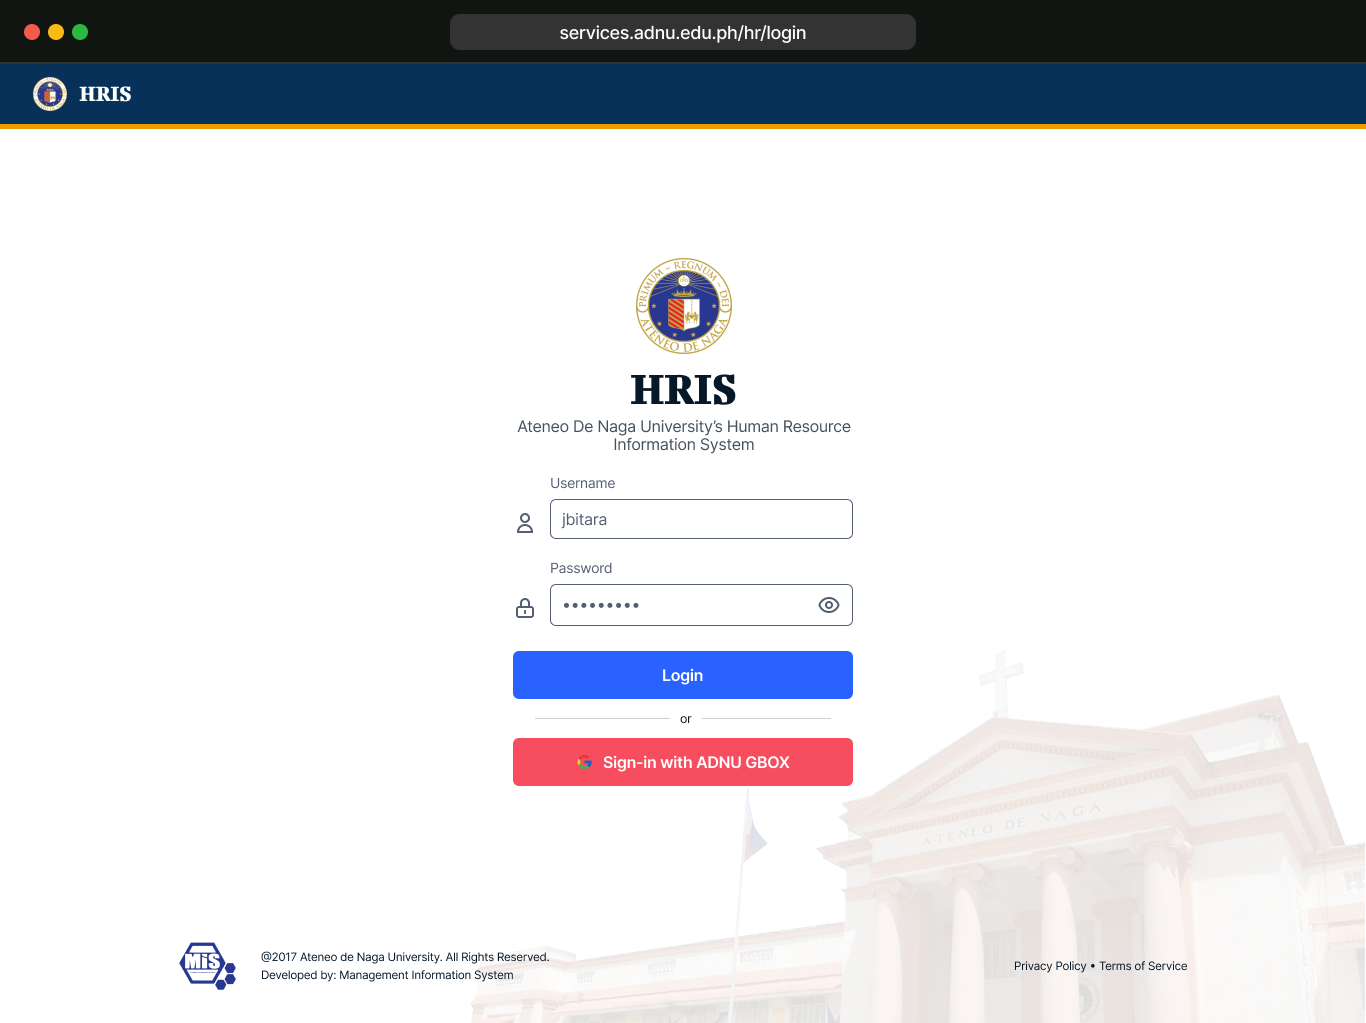
\includegraphics[width=1\linewidth]{figures/app/login.png}}
        \caption{Redesigned Login Page.}
        \label{fig:app-login}
    \end{figure}

    The new HRIS shall include an authentication module to handle HR managers i.e., Director, Administrative Assistant, Capability Building Officer, Compensation \& Benefits Officer, Information Support Systems Officer, Consultant, Recruitment Staff, Training \& Development Specialist, Benefits and Wellness Specialist, Attendance Monitoring Staff, College
    
    Within this page, users can input their University account credentials or login through the use of their GBOX account.

    \begin{figure}[H]
        \centering
        \frame{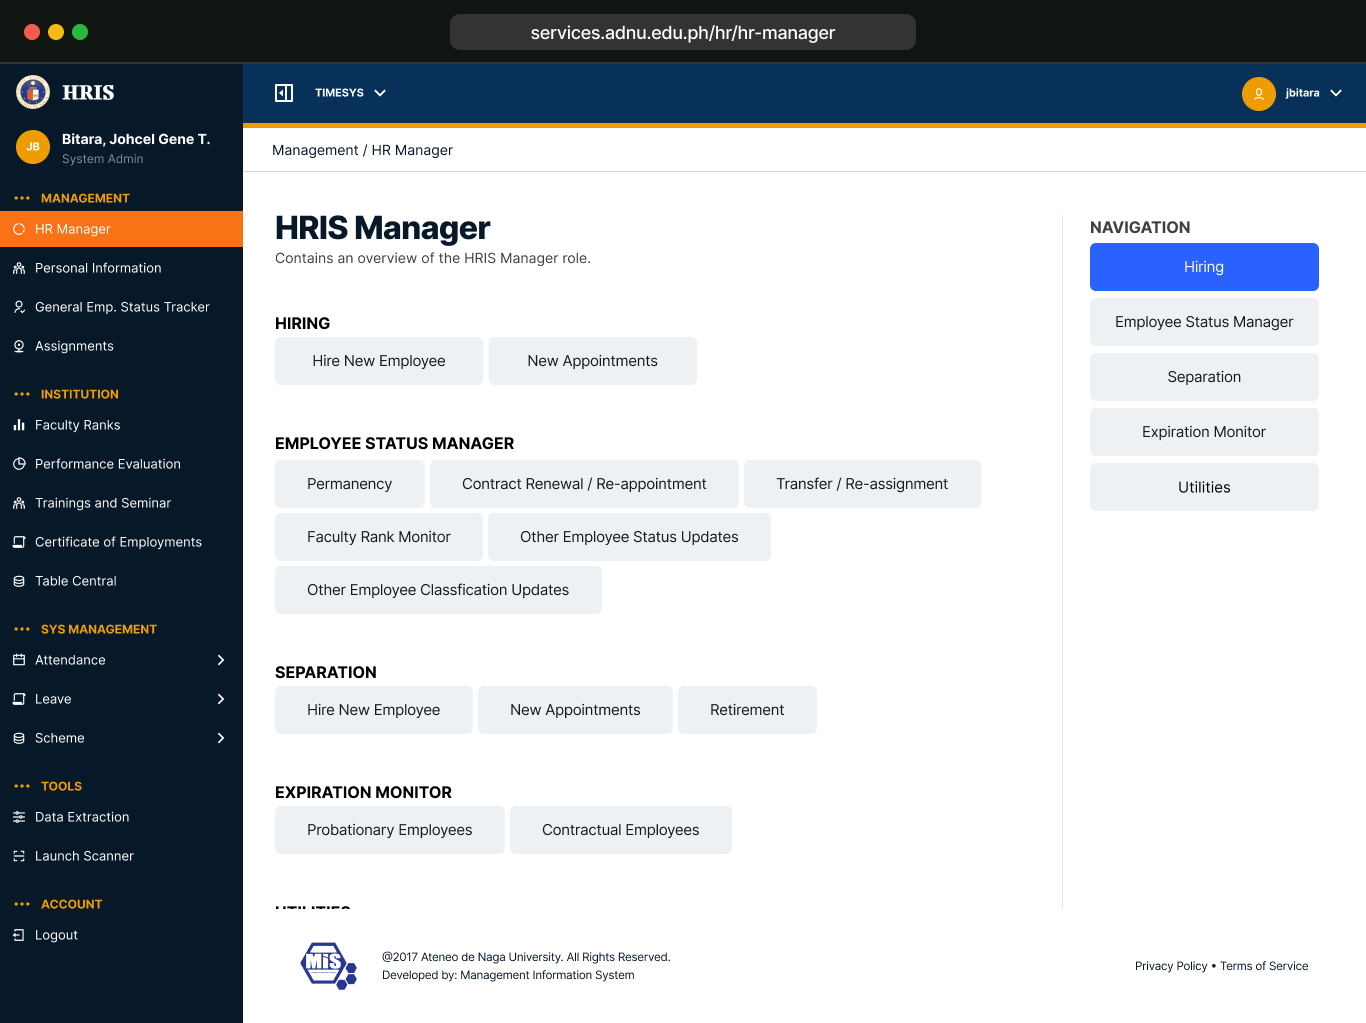
\includegraphics[width=1\linewidth]{figures/app/dashboard.png}}
        \caption{Redesigned Dashboard Page.}
        \label{fig:app-manager}
    \end{figure}

    Within this page, is the default home page for all HR managers. This page displays the summary of the HRIS system and the current status of the HRIS system. This includes a visualized Key Performance Indicators (KPIs) of the system's data and the current status of the system along with clickable links for different modules.

    \begin{figure}[H]
        \centering
        \frame{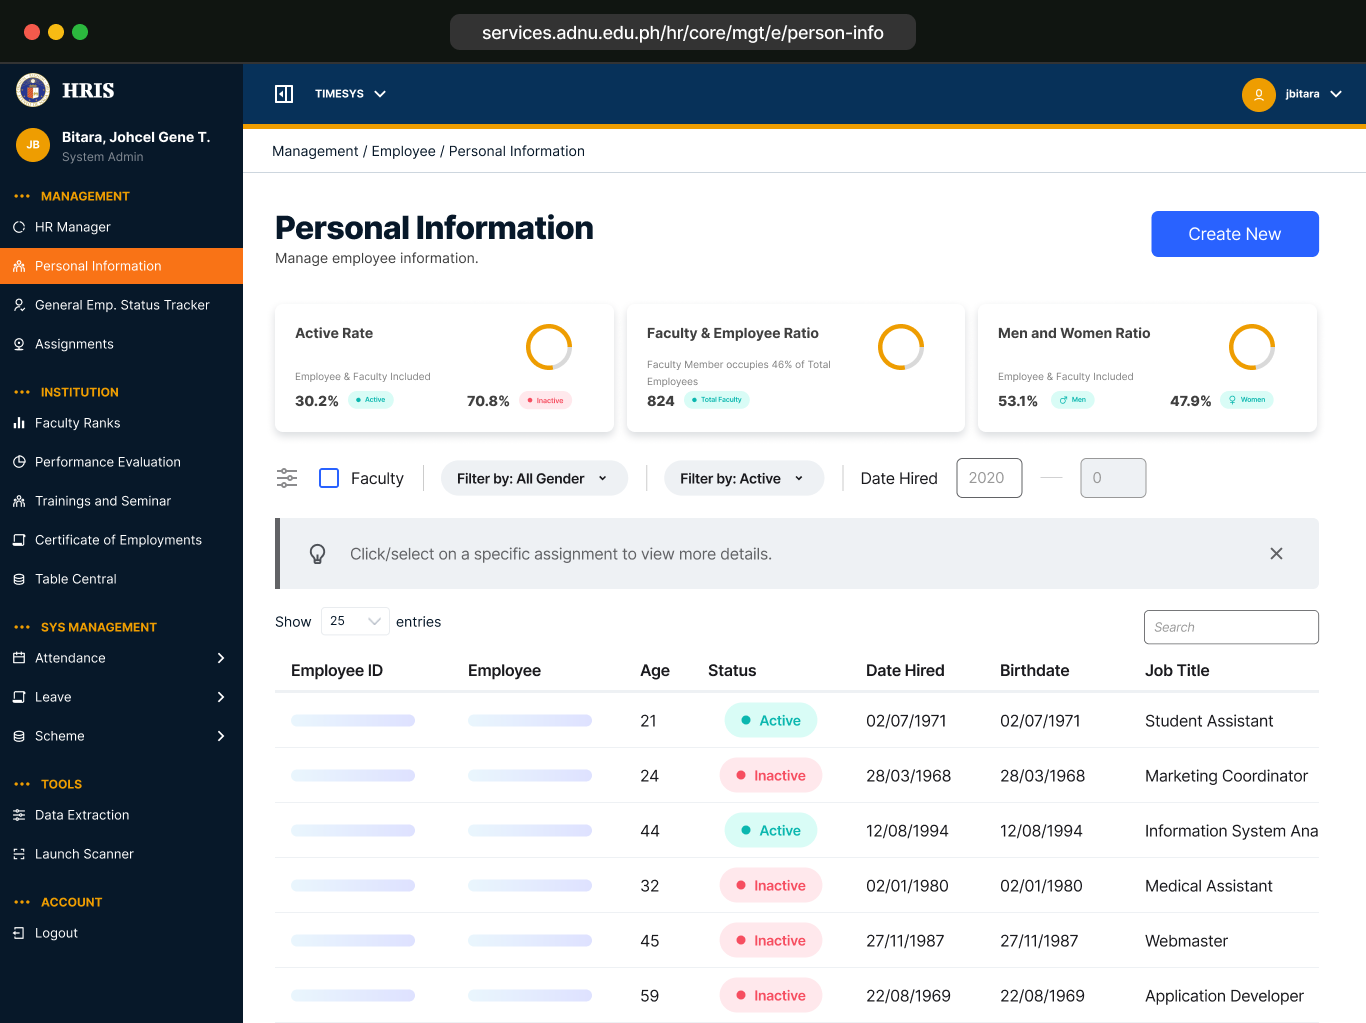
\includegraphics[width=1\linewidth]{figures/app/pi.png}}
        \caption{Redesigned Personal Information for All Employees.}
        \label{fig:app-pi}
    \end{figure}

    Within this page displays all the basic personal information for all employees in table view. This includes their personal information. Admins can select or filter among the employees to view more of their personal information.

    \begin{figure}[H]
        \centering
        \frame{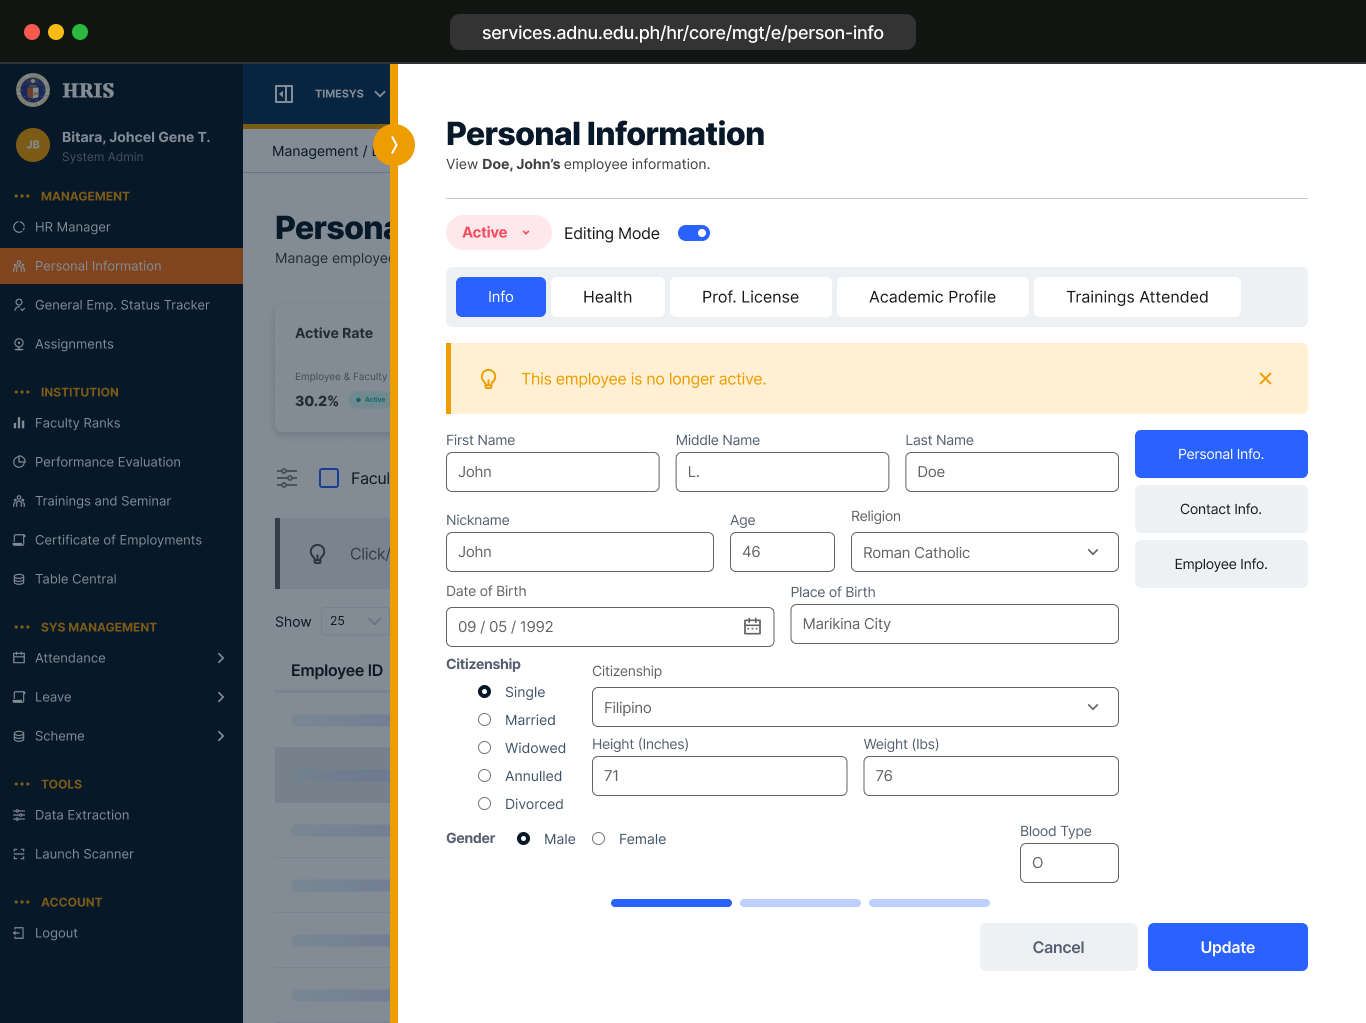
\includegraphics[width=1\linewidth]{figures/app/pi-info.png}}
        \caption{Viewing of Personal Information on Selected Employee.}
        \label{fig:app-pi-info}
    \end{figure}

    Upon selecting an employee, the page displays the interface for viewing/managing of the selected personal information in the record. Admins with access privileges can manage personal information for each employee  in the system.

    \begin{figure}[H]
        \centering
        \frame{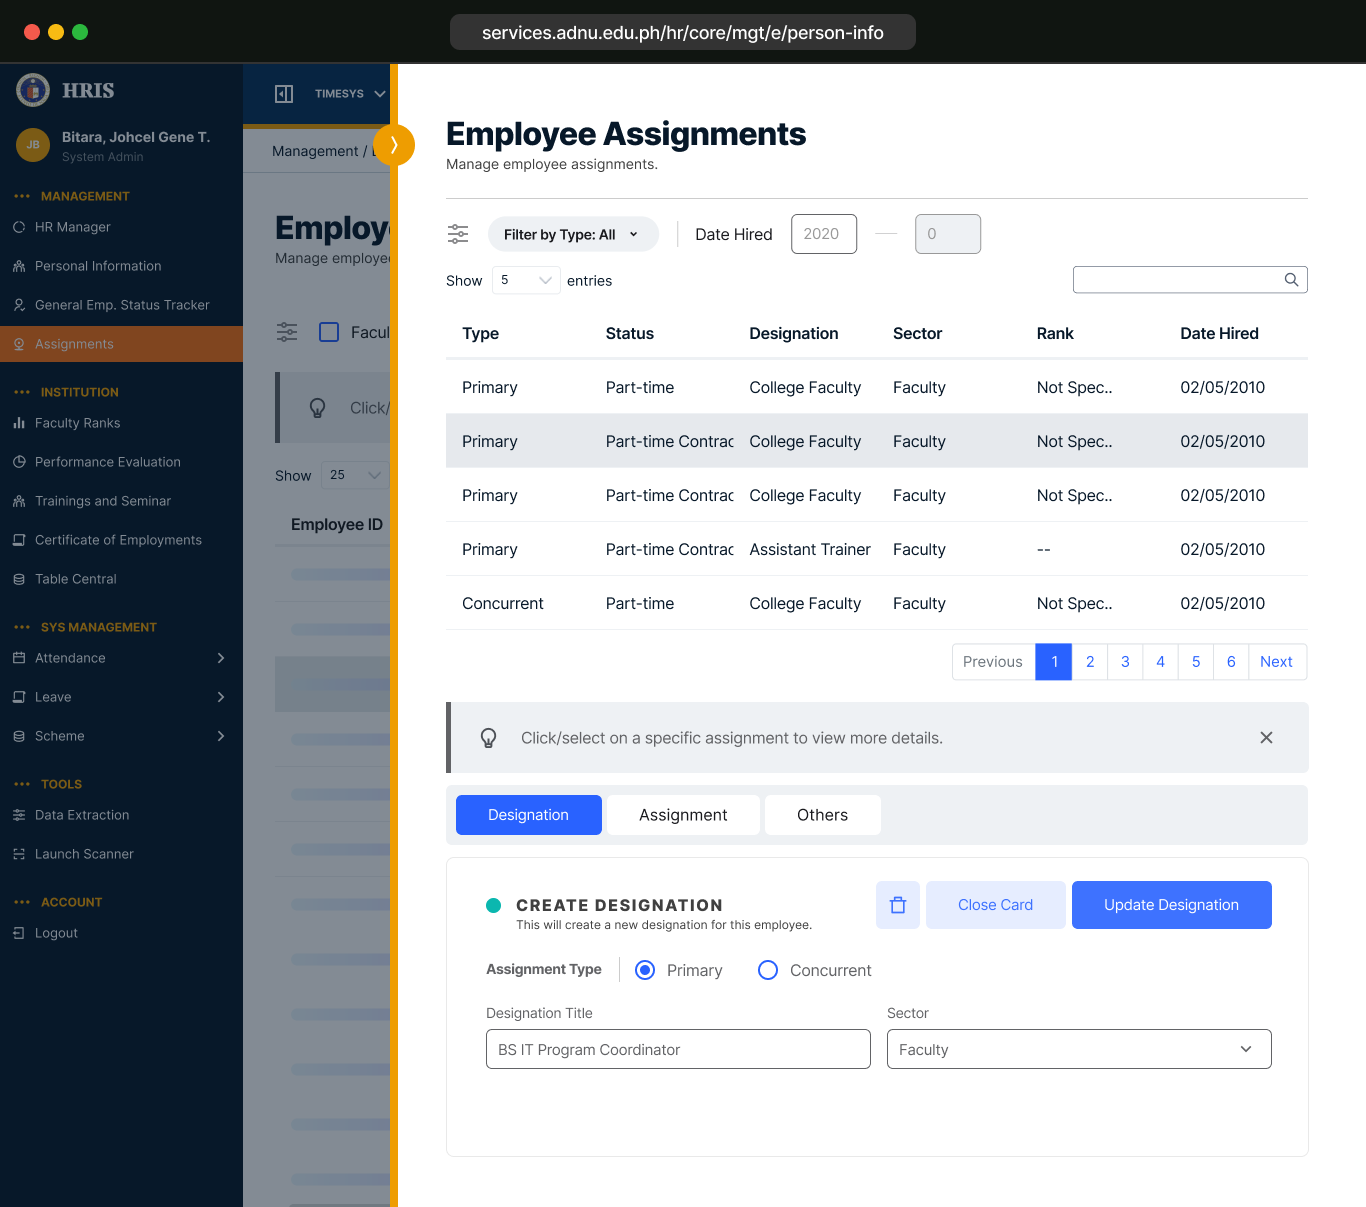
\includegraphics[width=1\linewidth]{figures/app/assignment.png}}
        \caption{Redesigned Employee Assignment Page.}
        \label{fig:app-assignment}
    \end{figure}

    Part of the crucial components of the system is managing employee designations and assignments. This page displays the interface for managing employee assignments and designations. Admins can assign employees to specific roles, office unit designation, create remarks, and employment status.

    \begin{figure}[H]
        \centering
        \frame{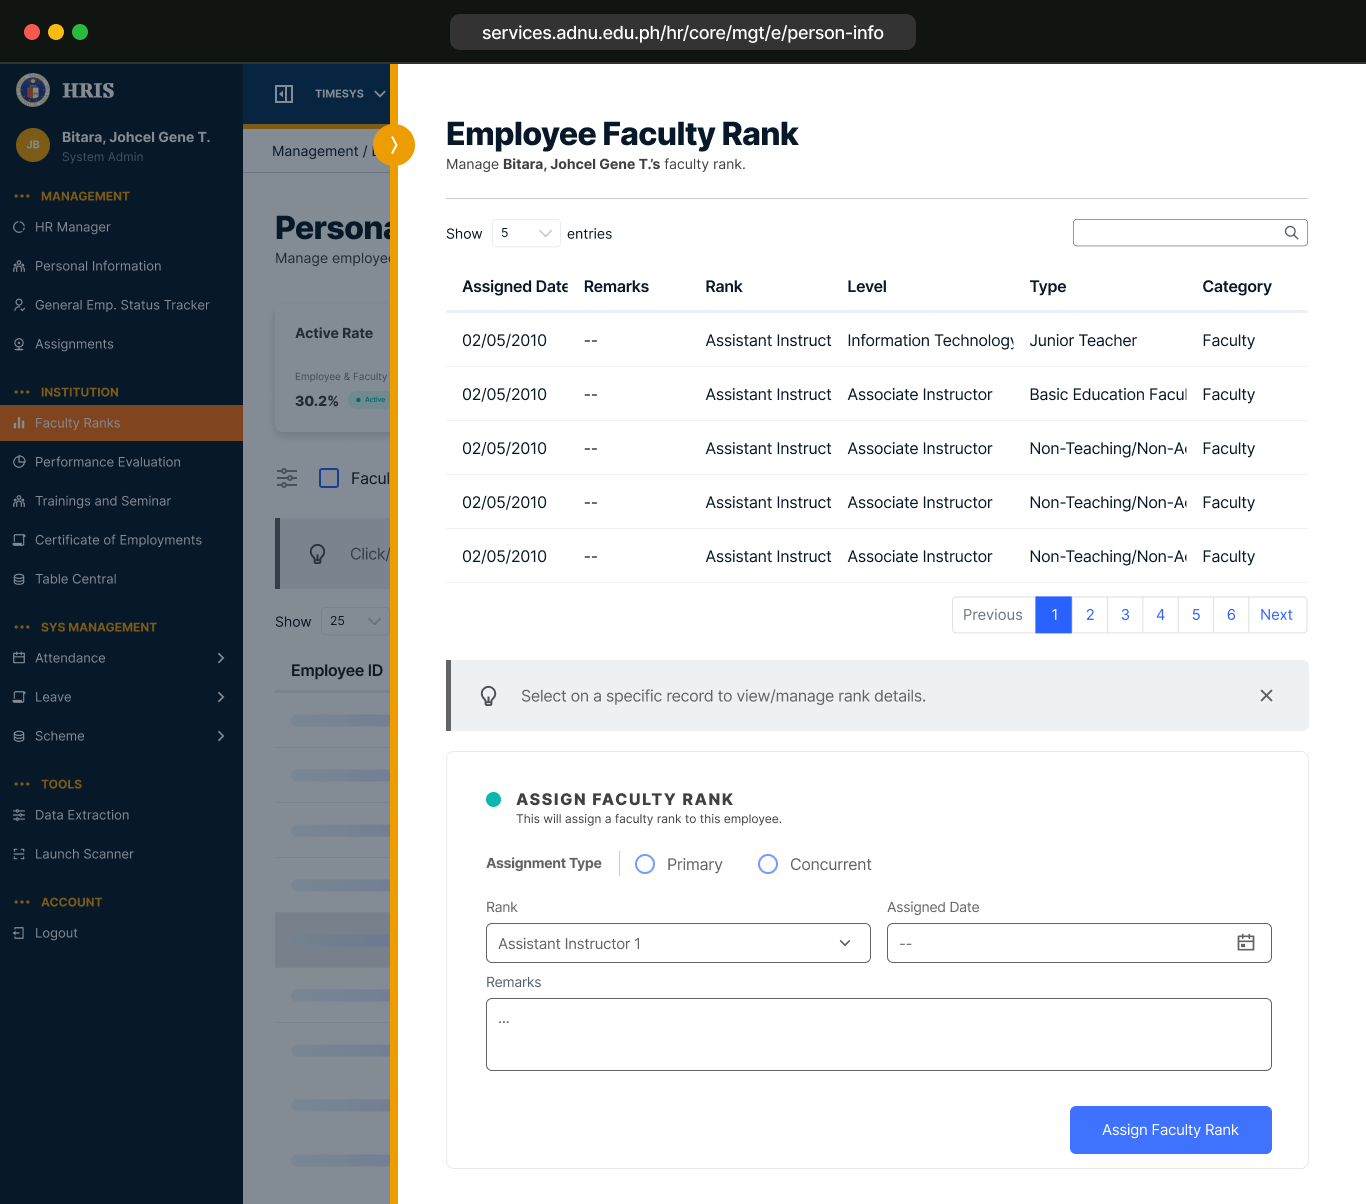
\includegraphics[width=1\linewidth]{figures/app/ranks.png}}
        \caption{Redesigned Faculty Rank Page.}
        \label{fig:app-fac-rank}
    \end{figure}

    This page displays the interface for managing faculty ranks. Similarly with managing employee information and assignments, the admin selects among the table and a sidebar will display the information for the selected faculty member.
    
    Admins can assign faculty members to specific ranks, rank levels, and rank types. This page also includes functionalities for tracking rank changes and historical data.

    \begin{figure}[H]
        \centering
        \frame{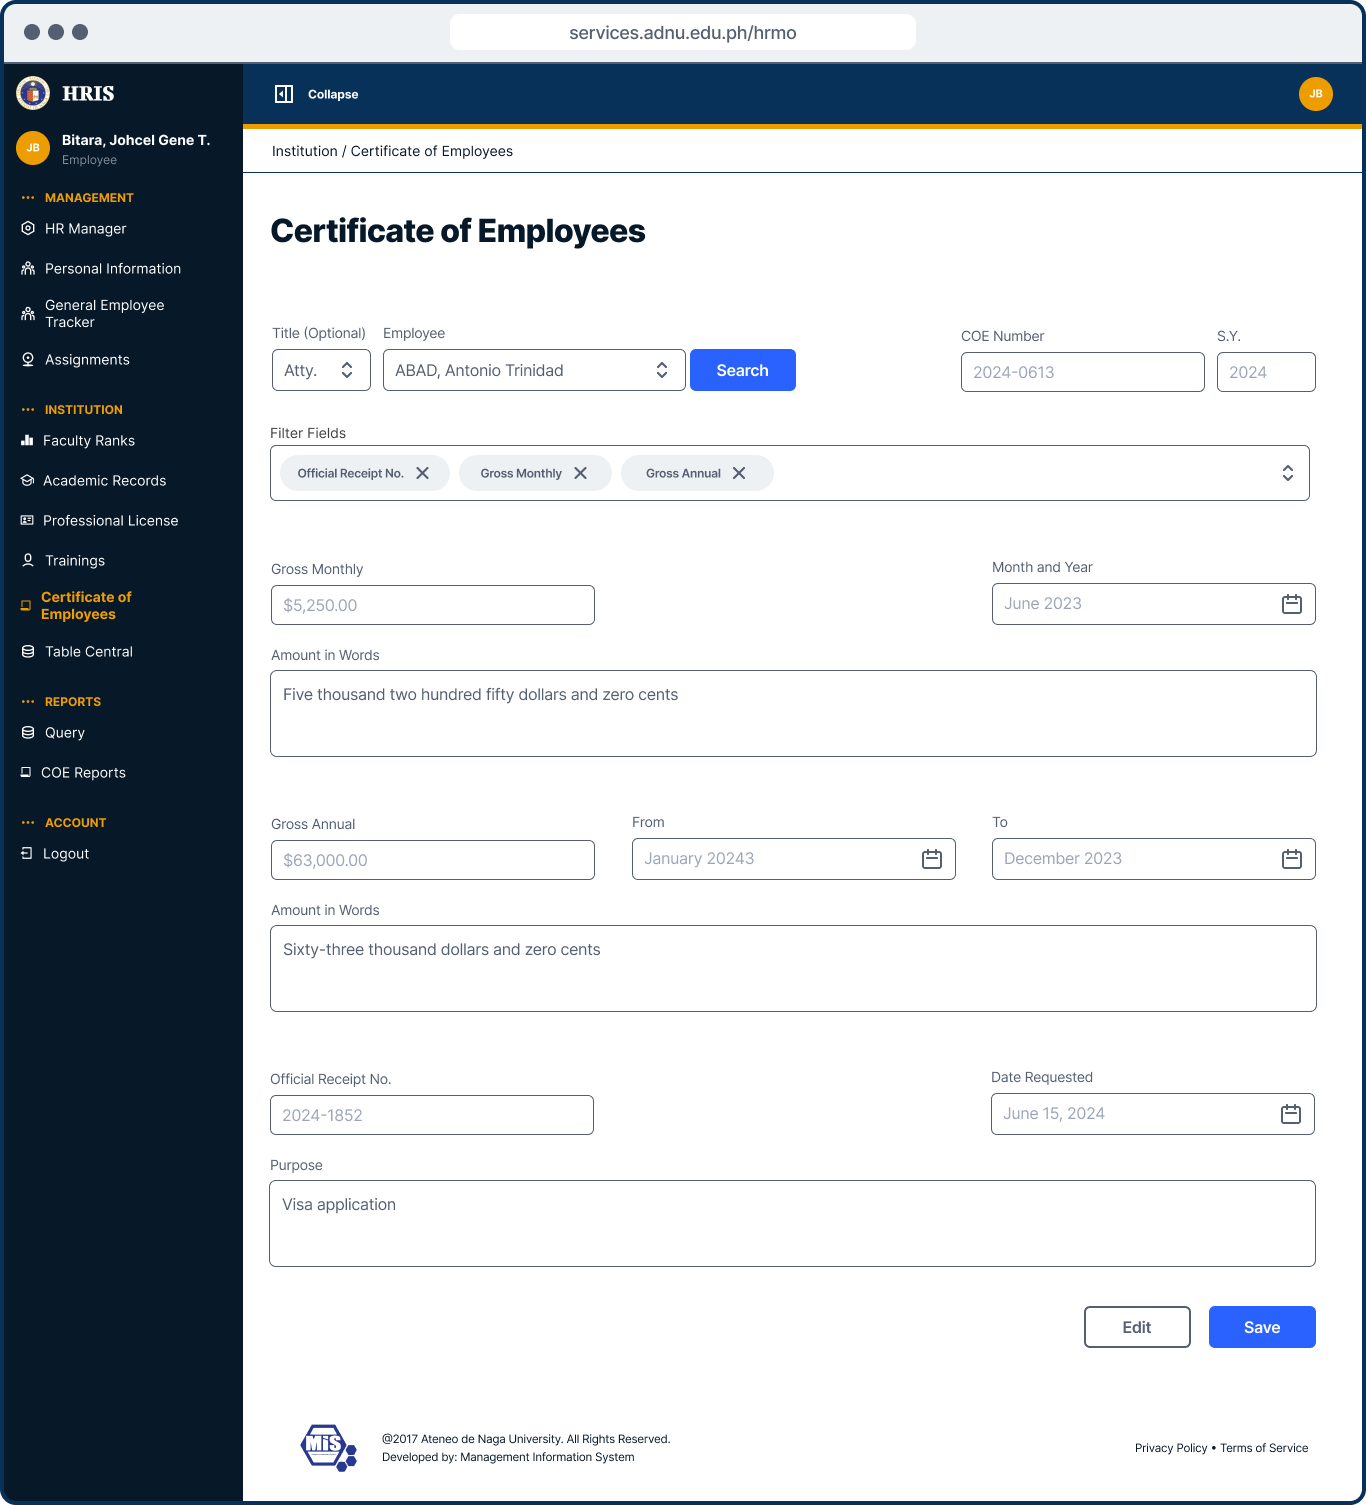
\includegraphics[width=1\linewidth]{figures/app/coe.png}}
        \caption{Redesigned Certificate of Employment Page.}
        \label{fig:app-coe}
    \end{figure}

    This page displays the interface for managing and generating newly issued or history of Certificates of Employment (COE). Within this page, admins can select or filter among the entries from the table and view the details of the selected COE. 

    \begin{figure}[H]
        \centering
        \frame{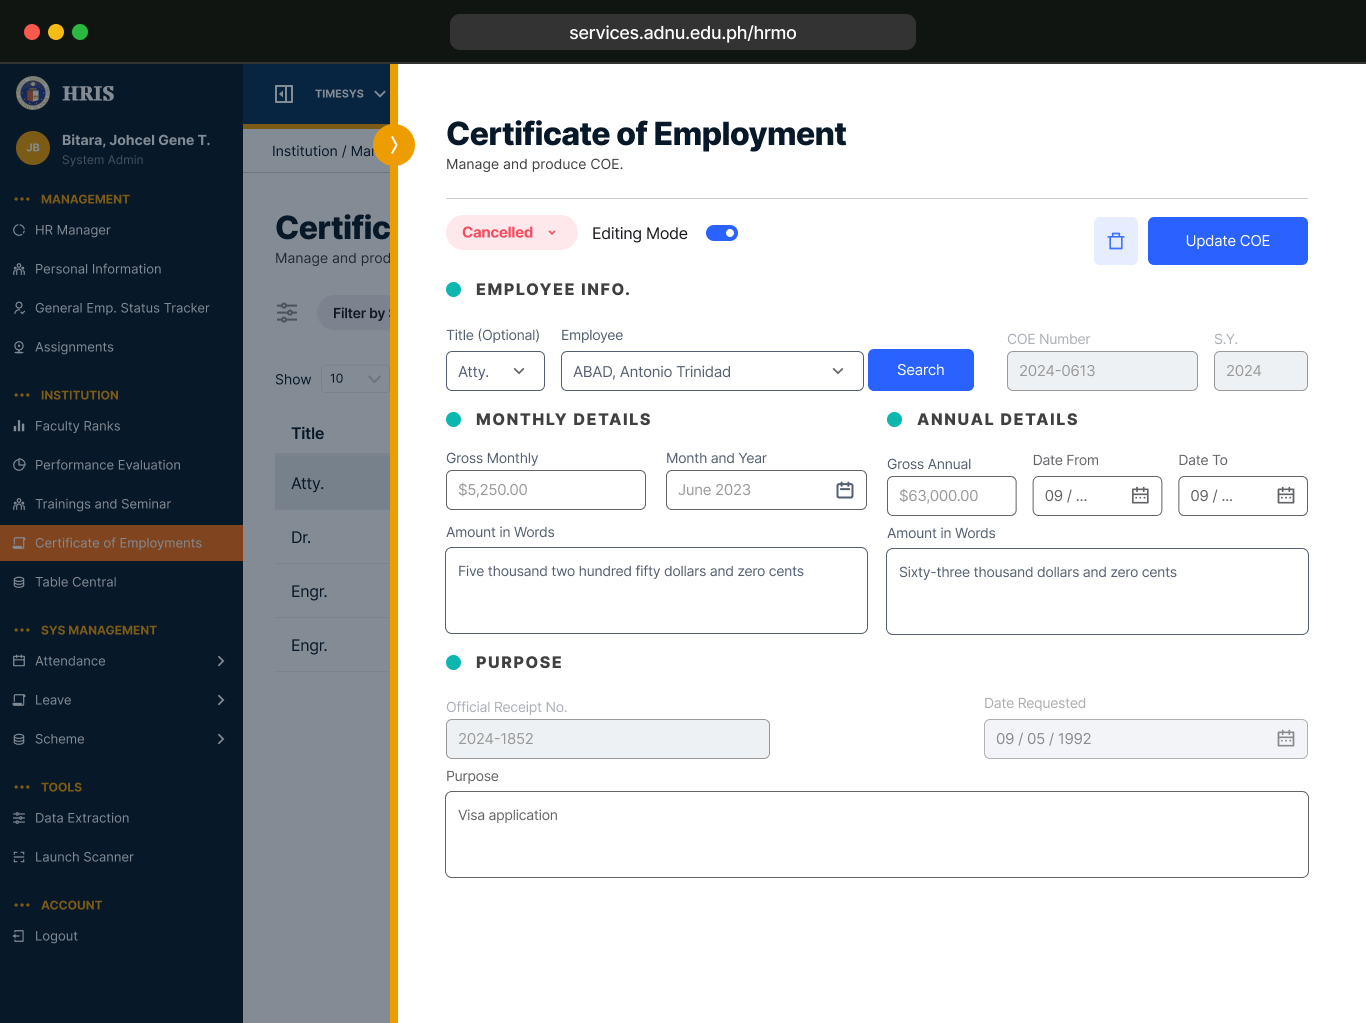
\includegraphics[width=1\linewidth]{figures/app/coe-info.png}}
        \caption{New HRIS Certificate of Employment Processing Page.}
        \label{fig:app-coe-info}
    \end{figure}

    Upon selecting a COE, the page displays the interface for viewing/managing of the selected COE in the record. Admins with access privileges can manage COE information for each employee in the system.

    \begin{figure}[H]
        \centering
        \frame{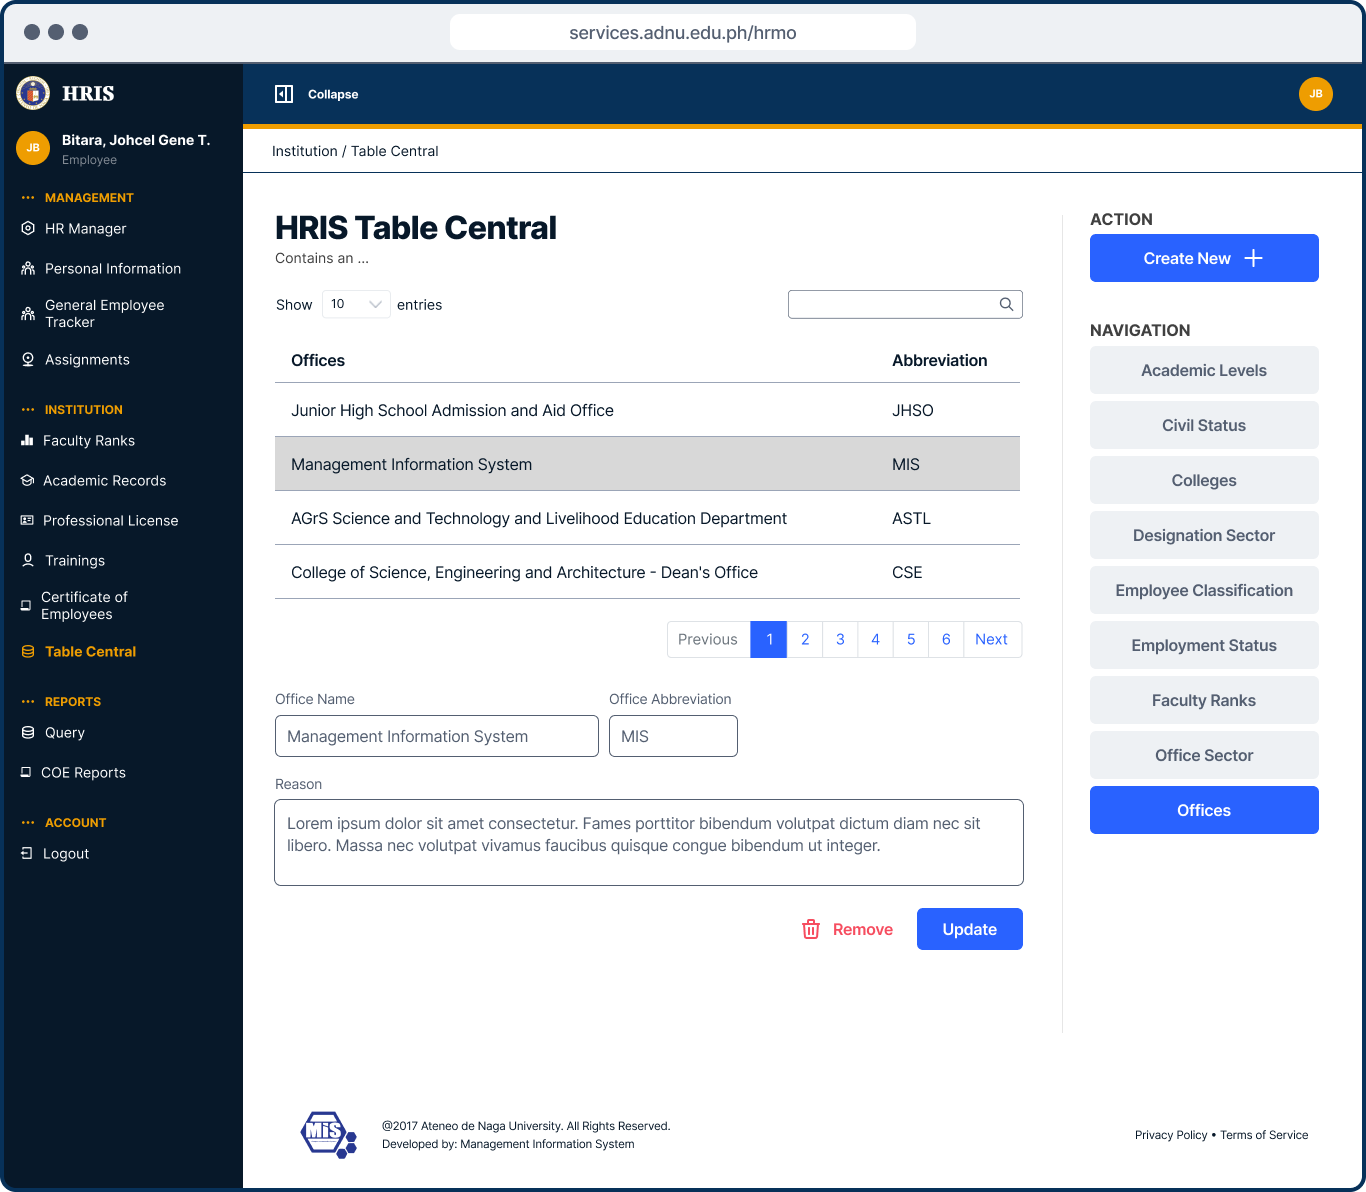
\includegraphics[width=1\linewidth]{figures/app/table-central.png}}
        \caption{Redesigned Table Central Page.}
        \label{fig:app-table-central}
    \end{figure}

    Within this page displays the HRIS Table Central module wherein, managers can manage certain sectors and department information and make updates within the schema's base tables. This includes the office type, office unit, office sector, academic levels, civil statuses, colleges, designation sectors, employee classification, employment status, and faculty ranks. which are used in reference to the HR's data as well on other University's systems.

    \begin{figure}[H]
        \centering
        \frame{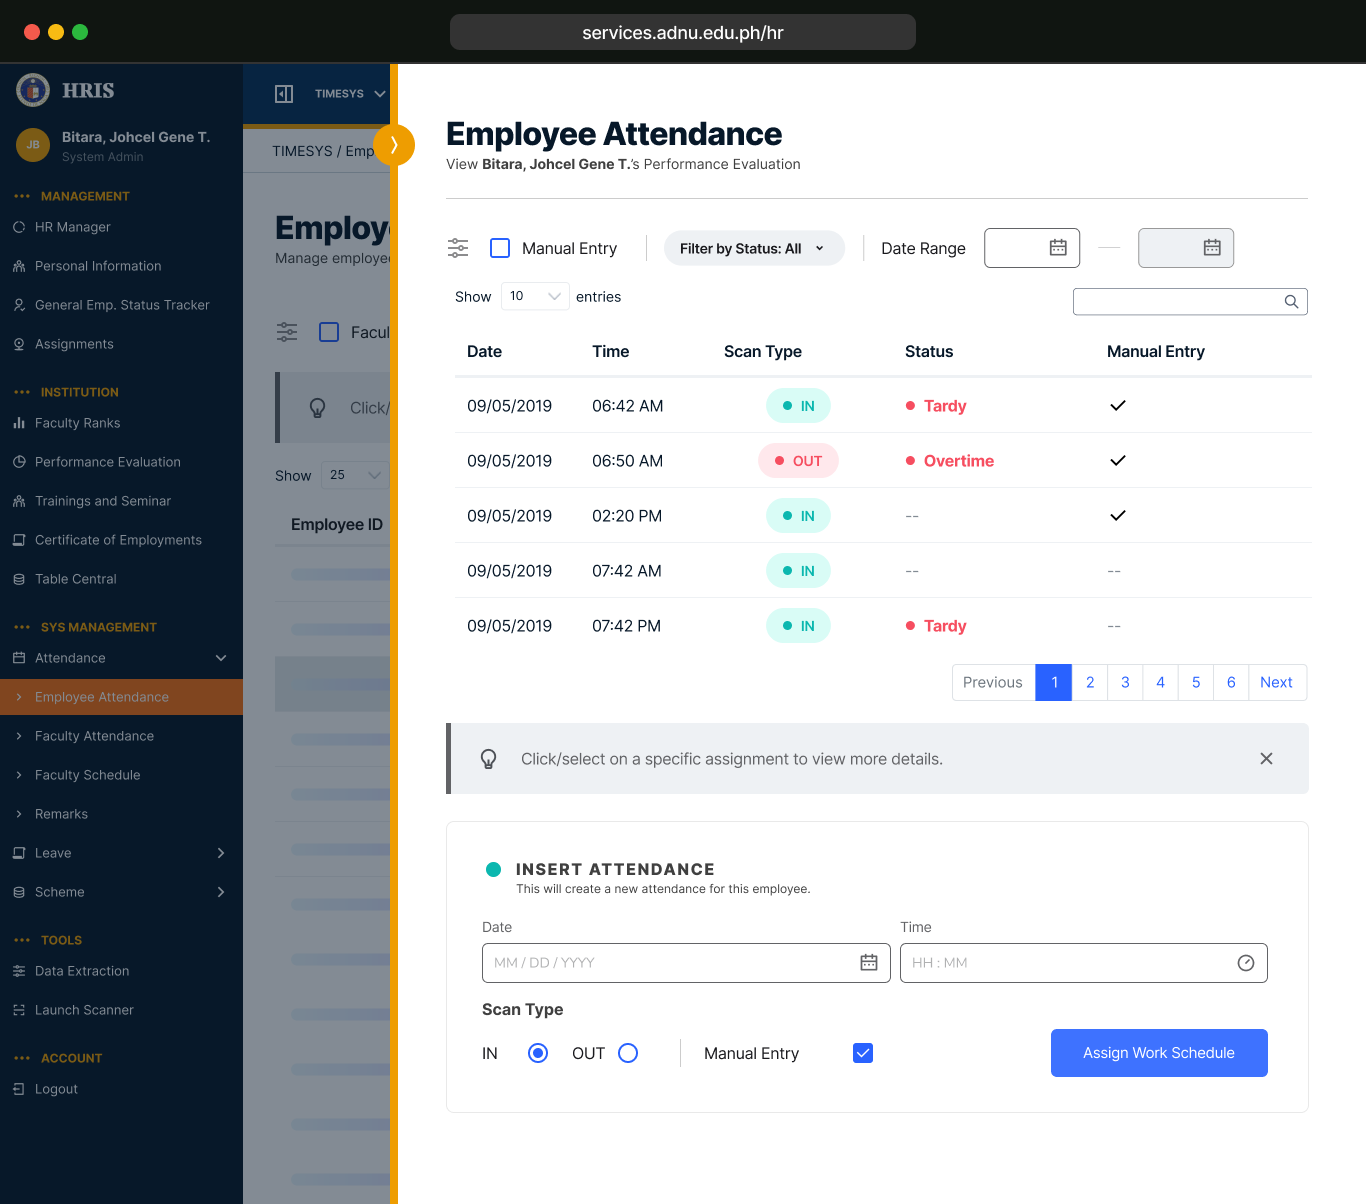
\includegraphics[width=1\linewidth]{figures/app/attendance-emp.png}}
        \caption{Redesigned Employee Attendance Management Page.}
        \label{fig:app-attendance-emp}
    \end{figure}

    Within this page displays the interface for managing employee attendance. This is in connection with the TIMESYS module and the DTR scanner. Records of employee attendance are displayed in table view, and admins can manage attendance records, including time-in/out, date, scan type and their computed status -- Tardy, Overtime, Absent, or Present.

    \begin{figure}[H]
        \centering
        \frame{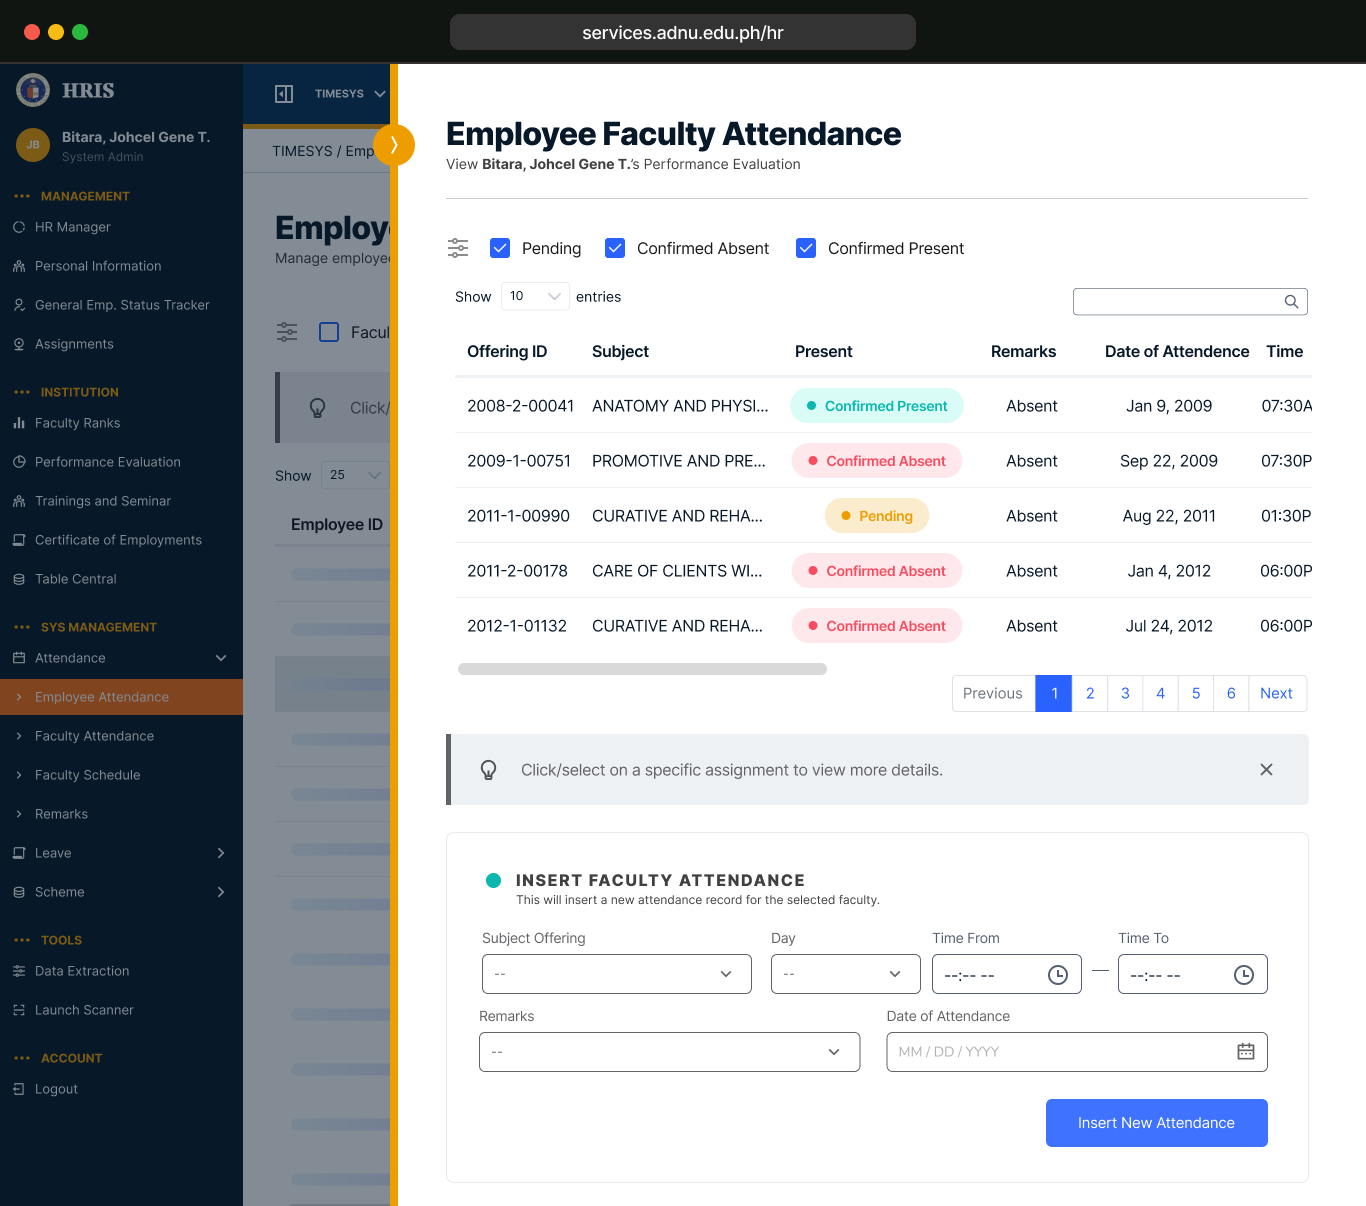
\includegraphics[width=1\linewidth]{figures/app/attendance-fac.png}}
        \caption{Redesigned Faculty Attendance Management Page.}
        \label{fig:app-attendance-fac}
    \end{figure}

    With this page displays the interface for managing faculty attendance. This is in connection with the FACSYS module. Records of faculty attendance are displayed in table view, and admins can manage attendance records, including the subject attended, day, remarks, and date of attendance.

    \begin{figure}[H]
        \centering
        \frame{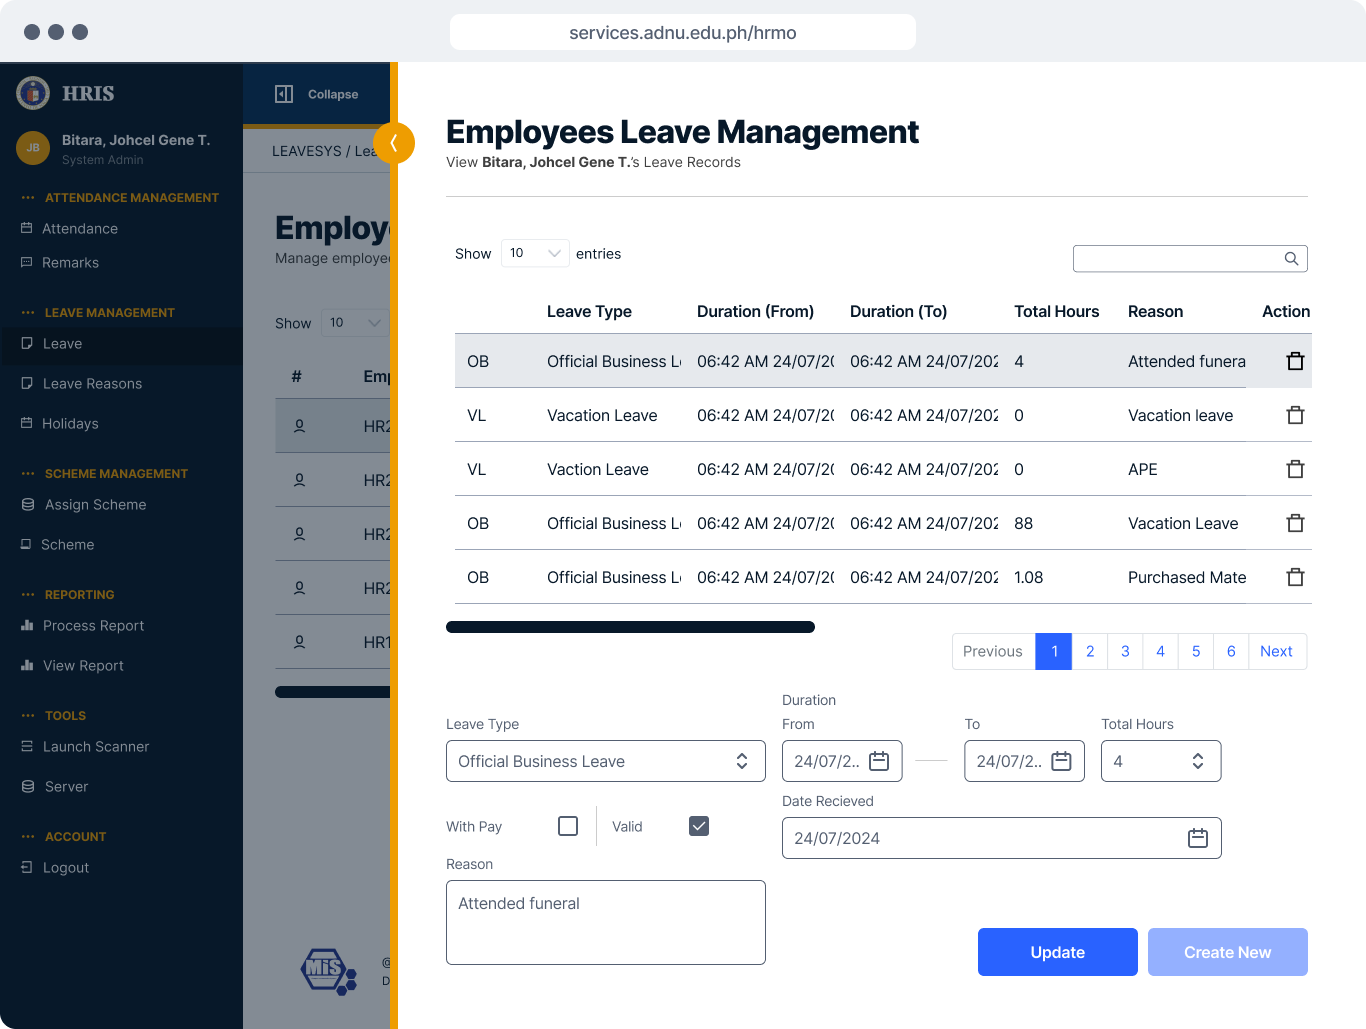
\includegraphics[width=1\linewidth]{figures/app/leave-mgt.png}}
        \caption{Redesigned Leave Management Page.}
        \label{fig:leave-mgt}
    \end{figure}

    Within this page, admins can manage filed employee leave applications and AWOLs. Admins can entry leave applications, view leave applications, and manage leave applications. This page also includes functionalities for tracking leave balances and leave credits of the selected employee.

    \begin{figure}[H]
        \centering
        \frame{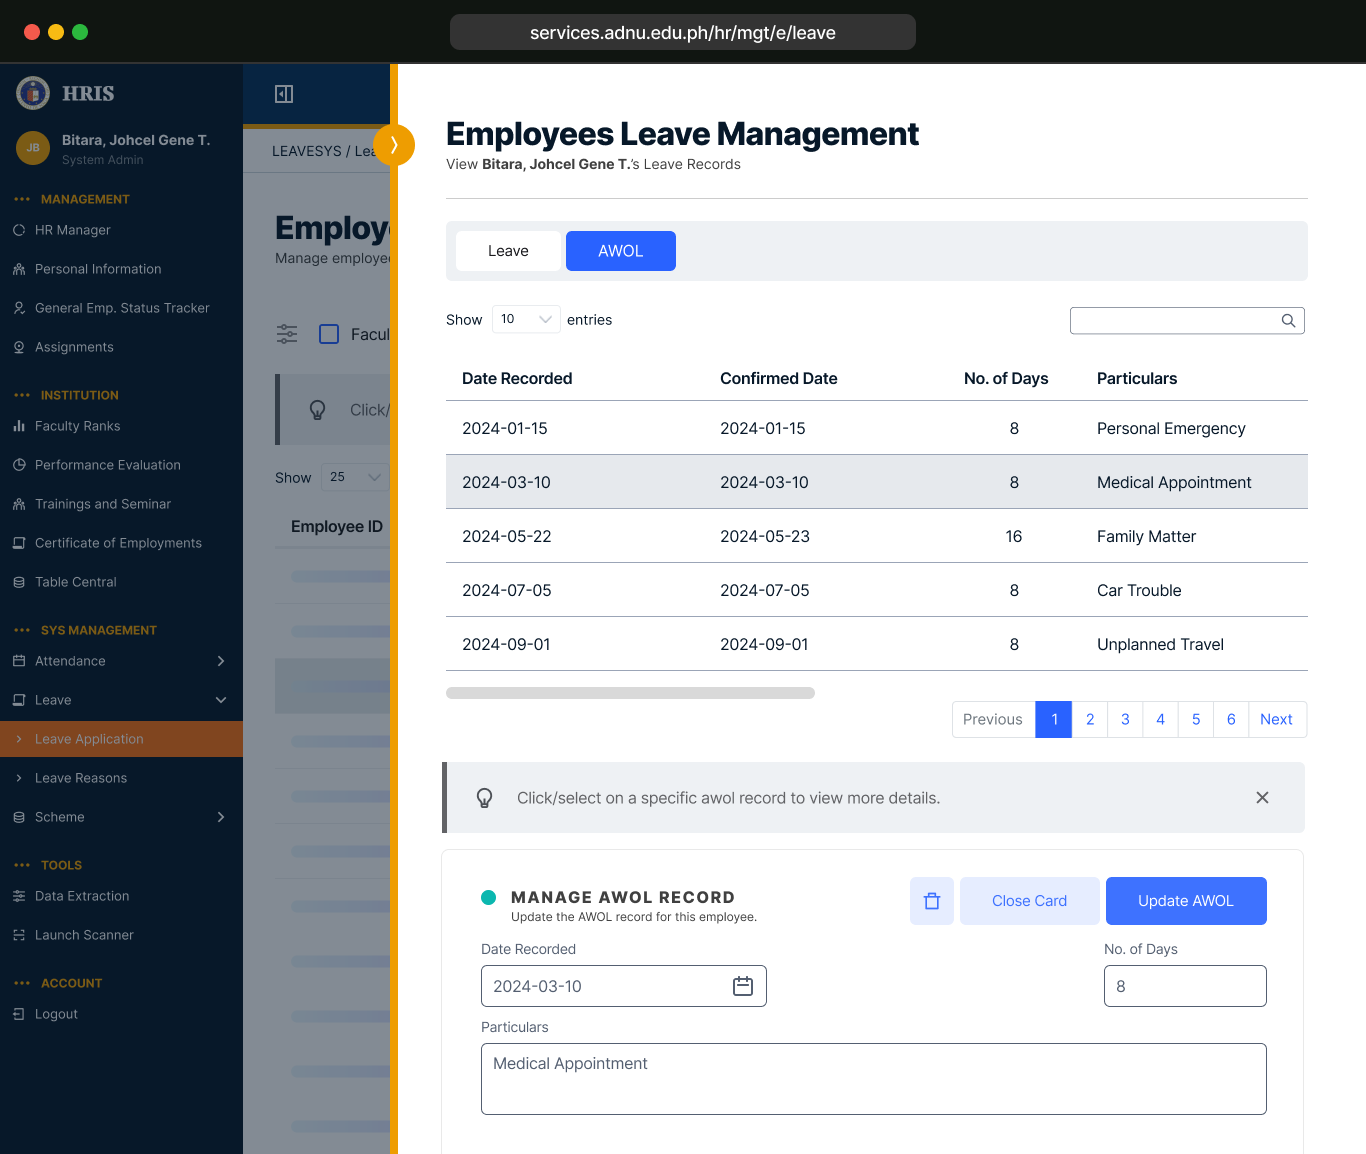
\includegraphics[width=1\linewidth]{figures/app/leave-awol.png}}
        \caption{New HRIS Employee AWOL Page.}
        \label{fig:leave-awol}
    \end{figure}

    Upon switching to the AWOL tab, the page displays the interface for managing and tracking Absent Without Leave (AWOL) records. In this section, admins can view, manage, and track AWOL records, including the date, particulars, confirmed date, and number of days.

    \begin{figure}[H]
        \centering
        \frame{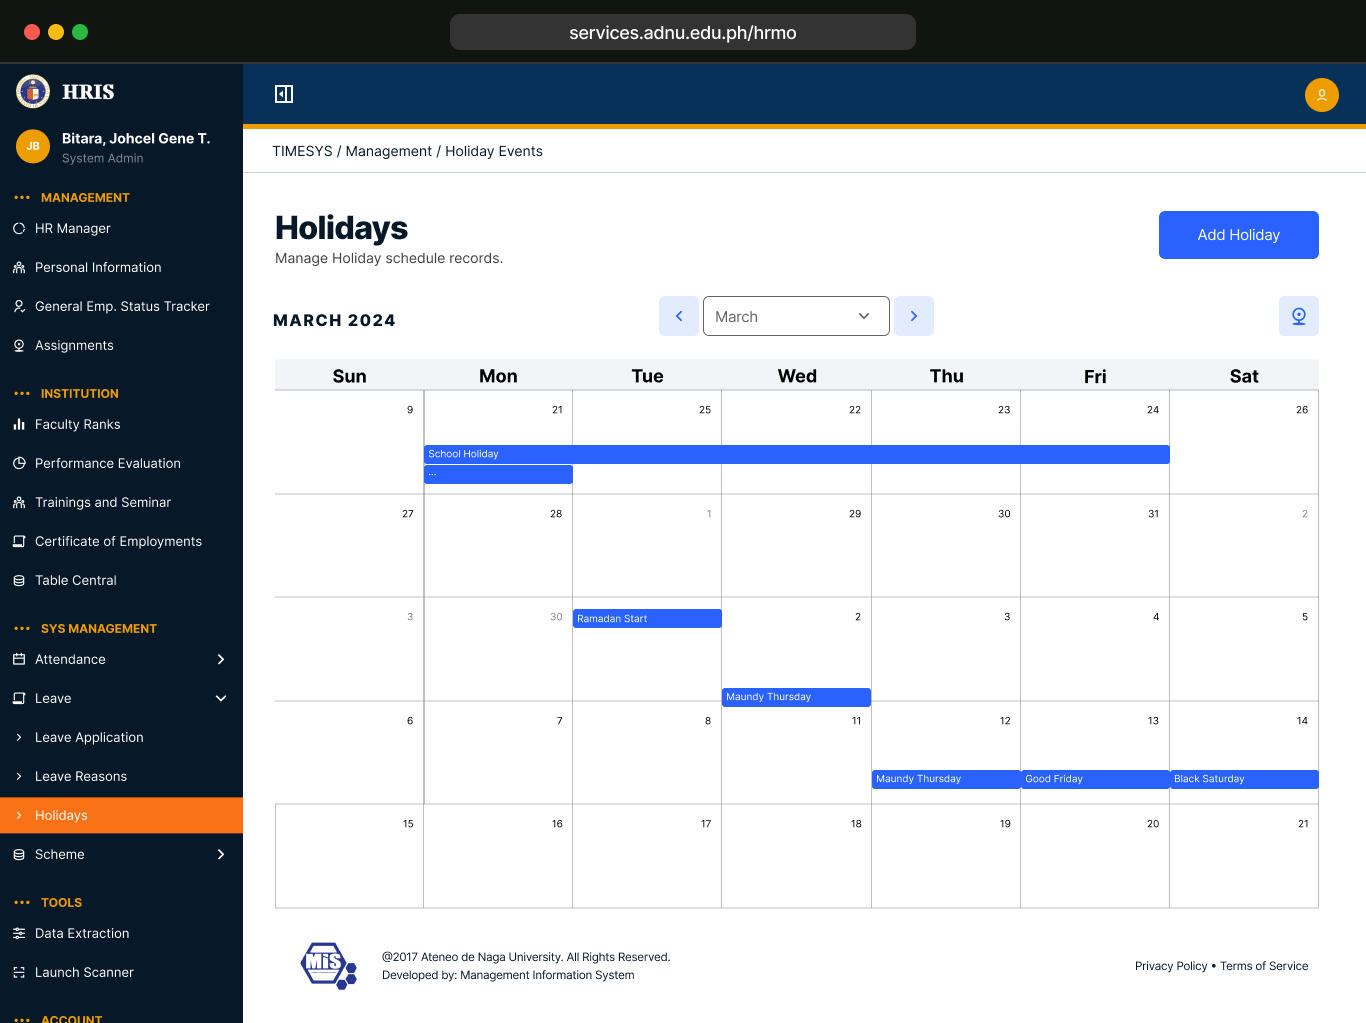
\includegraphics[width=1\linewidth]{figures/app/holiday.png}}
        \caption{Redesigned Holiday Management Page.}
        \label{fig:holiday}
    \end{figure}

    In this page, displays the management for holiday events. The interface provides a comprehensive view of the University's holiday schedules and non-working days. It includes functionalities for managing and updating holiday information with added optimization for their workflow by adding settings for recurrent dates.

    This record is crucial for the LEAVESYS and TIMESYS module as it is used to exclude non-working days from the leave computation and attendance monitoring.

    \begin{figure}[H]
        \centering
        \frame{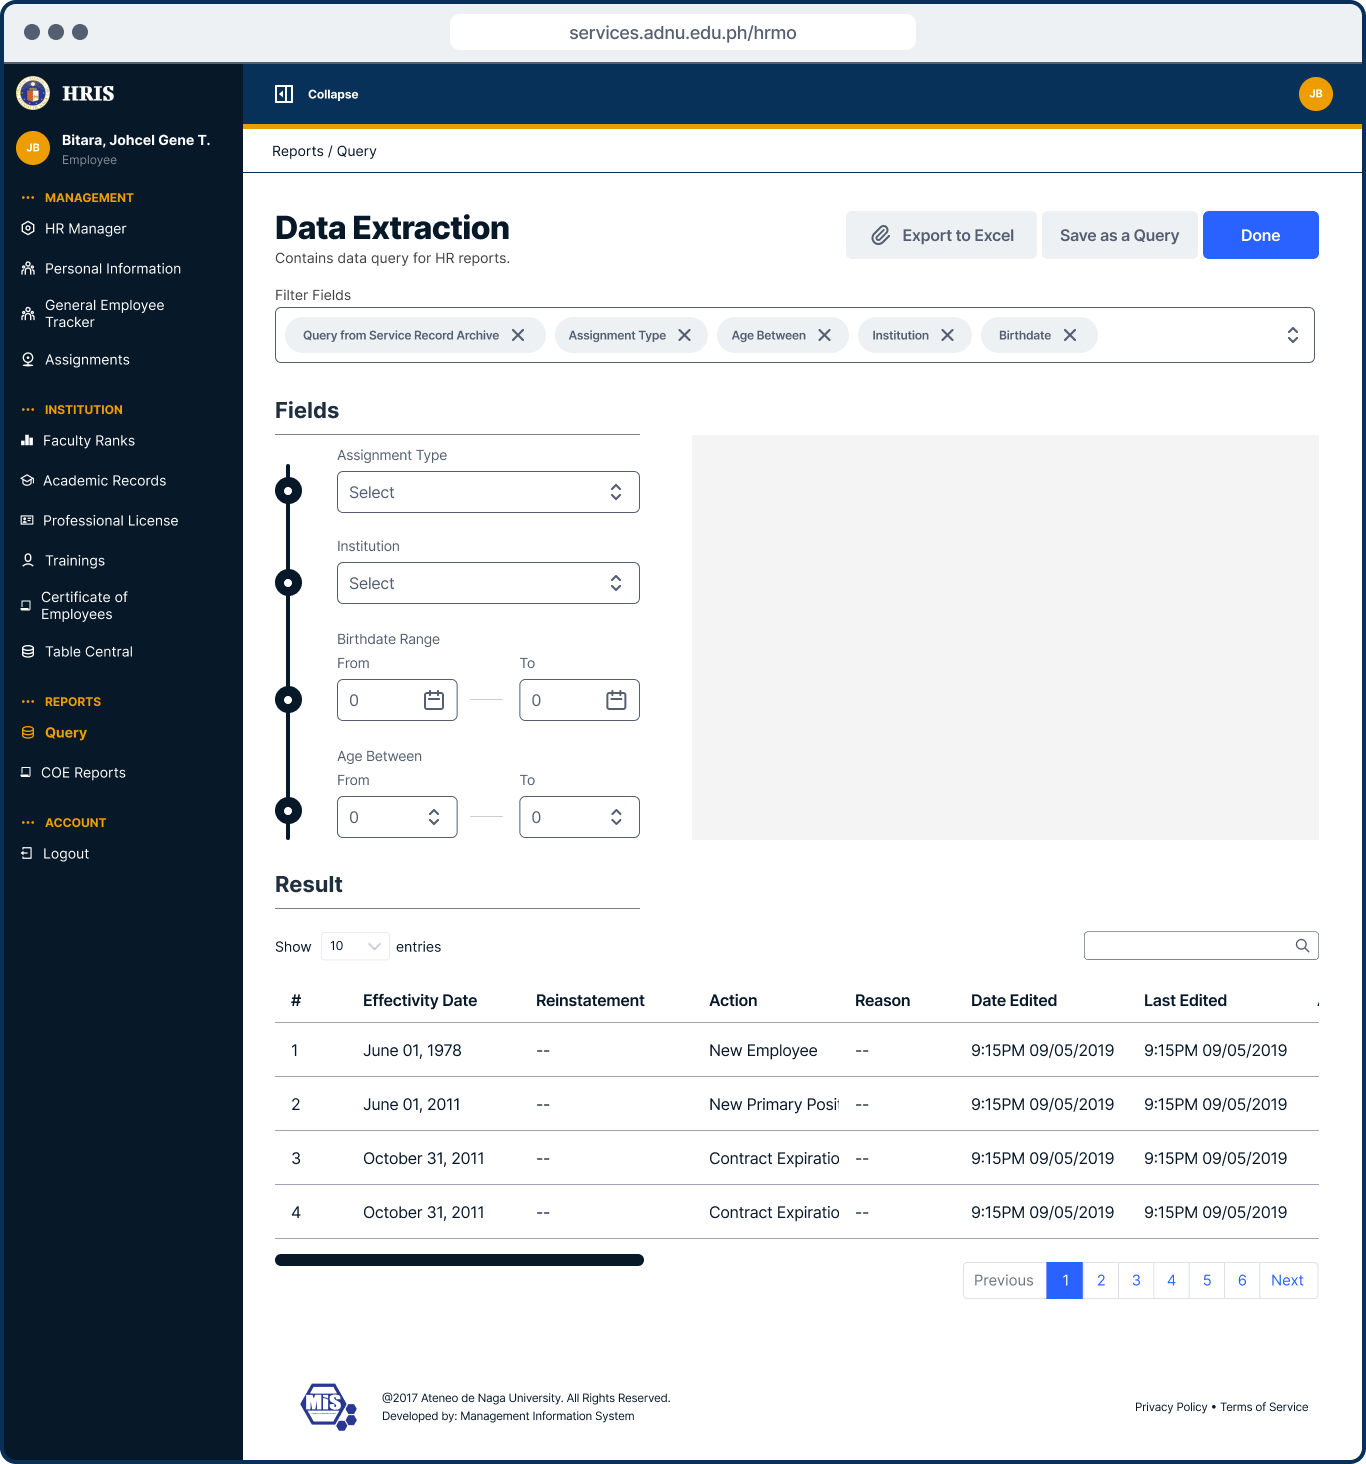
\includegraphics[width=1\linewidth]{figures/app/data-extraction.png}}
        \caption{Redesigned Data Extraction Page.}
        \label{fig:app-data-extraction}
    \end{figure}

    In this page, is the date extraction or query page for HR managers to extract reports. The interface is designed to facilitate efficient retrieval of HR data, likely offering options for customizable reports, data filtering, and exporting functionalities in Excel or CSV format.

    \begin{figure}[H]
        \centering
        \frame{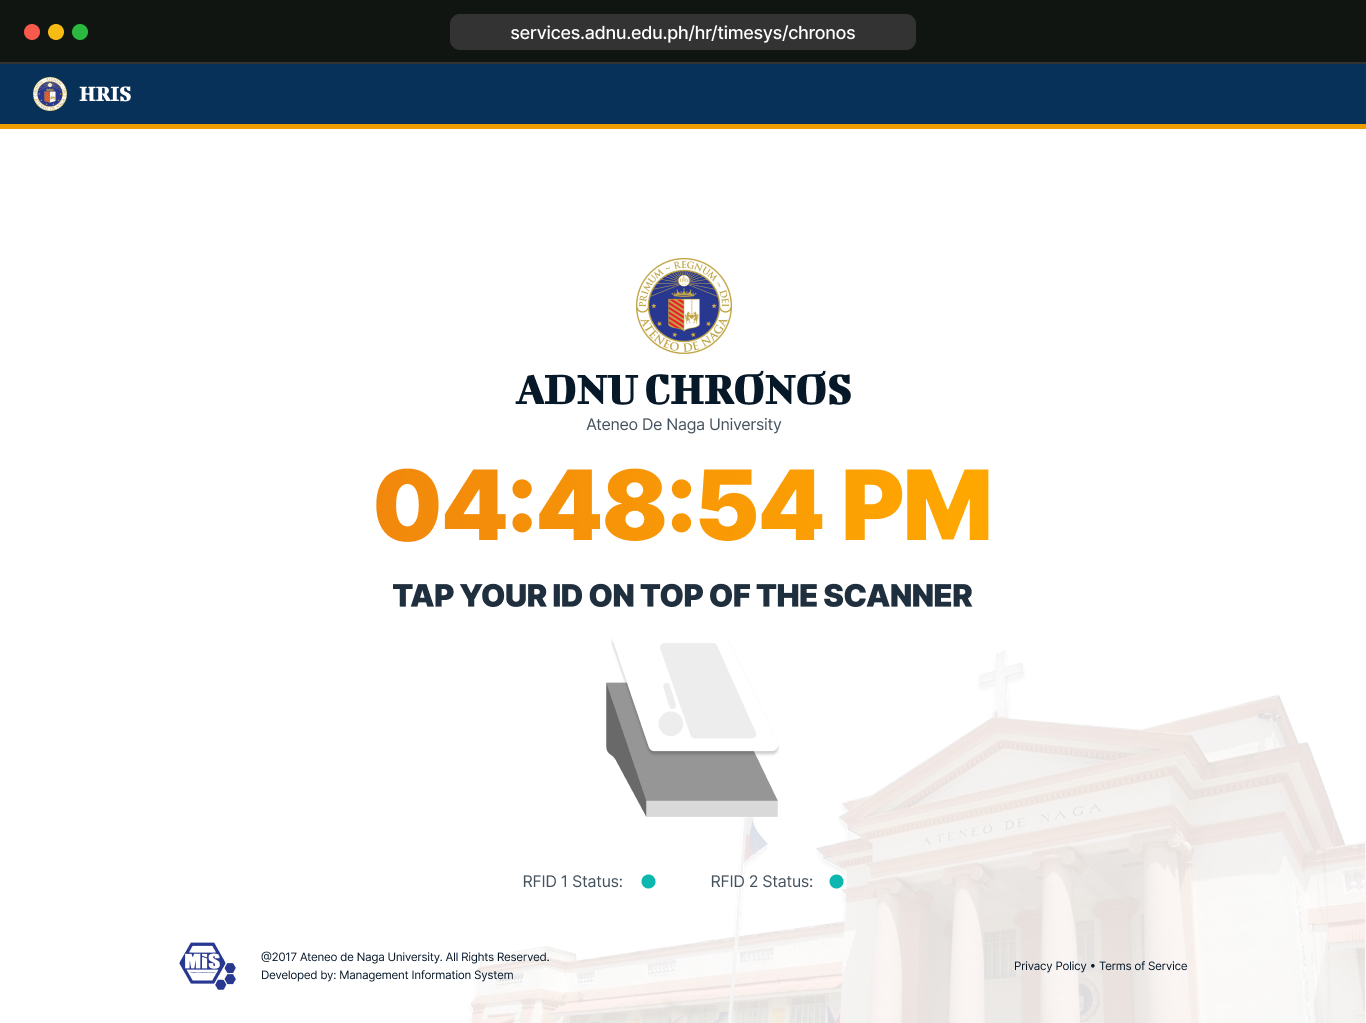
\includegraphics[width=1\linewidth]{figures/app/chronos.png}}
        \caption{Redesigned Chronos Page.}
        \label{fig:app-chronos}
    \end{figure}

    The CHRONOS is designed as an interface for employee attendance in connection with DTR scanner devices to record employee attendance by scanning/tapping their ID cards. This record is then used to compute for the employee's tardiness, overtime, and absences in the figure \ref*{fig:app-attendance-emp}.